% IEEE Paper Template for US-LETTER Page Size (V1)
% Sample Conference Paper using IEEE LaTeX style file for US-LETTER pagesize.
% Copyright (C) 2006-2008 Causal Productions Pty Ltd.
% Permission is granted to distribute and revise this file provided that
% this header remains intact.
%
% REVISION HISTORY
% 20080211 changed some space characters in the title-author block
%
\documentclass[10pt,conference,letterpaper]{IEEEtran}
\usepackage{times,amsmath,epsfig}
\usepackage{algorithm}
\usepackage{algorithmic}
\usepackage{epstopdf}
\usepackage{graphicx}
\renewcommand{\algorithmicrequire}{\textbf{Input:}} 
\renewcommand{\algorithmicensure}{\textbf{Output:}}
\usepackage[tight,footnotesize]{subfigure}
\usepackage{amsfonts}
\usepackage{xspace}
\usepackage{bbm}

\newcommand{\tabincell}[2]{\begin{tabular}{@{}#1@{}}#2\end{tabular}}  
\newcommand{\frname}{GAT\xspace }
\newcommand{\idxname}{GTIDX\xspace }
\newcommand{\rangeq}{{{\cal Q}_r}\xspace}
\newcommand{\simq}{{{\cal Q}_k}\xspace}
\newcommand{\rangecand}{{{\cal Q}_r^c}\xspace}
\newcommand{\simcand}{{{\cal Q}_k^c}\xspace}
\newcommand{\alltraj}{{{\cal T}}\xspace}
\newcommand{\edr}{{\delta}\xspace}
\newcommand{\allcell}{{\cal C}\xspace}
\newcommand{\allseg}{{\cal G}\xspace}
\newcommand{\trajcell}{{f_c}\xspace}
\newcommand{\trajtable}{{\cal S}\xspace}
\newcommand{\quadtree}{{\cal P}\xspace}
% \newcommand{\rangecandnode}{{{\cal C}_r^c}\xspace}
\newcommand{\trajindex}{{{\cal I}_T}\xspace}
\newcommand{\treeindex}{{{\cal I}_Q}\xspace}
\newcommand{\knownedr}{{{\cal L}_\edr}\xspace}


\newcommand{\bigoh}{{\rm O}\xspace}
\newcommand{\eat}[1]{}
\newtheorem{definition}{Definition}
\newtheorem{theorem}{Theorem}
\newtheorem{lemma}{Lemma}
\newtheorem{corollary}{Corollary}

%
\title{An Efficient GPU-accelerated Framework for Answering Trajectory Queries}
%
\author{%
% author names are typeset in 11pt, which is the default size in the author block
{Bowen Zhang{\small $~$}, Yanyan Shen{\small $~$}, Yanmin Zhu{\small $~$} }%
% add some space between author names and affils
\vspace{1.6mm}\\
\fontsize{10}{10}\selectfont\itshape
% 20080211 CAUSAL PRODUCTIONS
% separate superscript on following line from affiliation using narrow space
$^{}$\,Department of Computer Science and Engeneering, Shanghai Jiao Tong University\\
Shanghai, China 200240\\
\fontsize{9}{9}\selectfont\ttfamily\upshape
%
% 20080211 CAUSAL PRODUCTIONS
% in the following email addresses, separate the superscript from the email address 
% using a narrow space \,
% the reason is that Acrobat Reader has an option to auto-detect urls and email
% addresses, and make them 'hot'.  Without a narrow space, the superscript is included
% in the email address and corrupts it.
% Also, removed ~ from pre-superscript since it does not seem to serve any purpose
\{zbw0046,shenyy,yzhu\}@sjtu.edu.cn\\
% add some space between email and affil
\vspace{1.2mm}\\
\fontsize{10}{10}\selectfont\rmfamily\itshape
% 20080211 CAUSAL PRODUCTIONS
% separated superscript on following line from affiliation using narrow space \,
%$^{*}$\,Second Company\\
%Address Including Country Name\\
%\fontsize{9}{9}\selectfont\ttfamily\upshape
%% 20080211 CAUSAL PRODUCTIONS
%% removed ~ from pre-superscript since it does not seem to serve any purpose
%$^{2}$\,second.author@second.com
}
%
\begin{document}
\maketitle
%
\begin{abstract} 
The last decade has witnessed the increasing amount of trajectory data, facilitating a wide spectrum of interesting applications. 
%The last decade has witnessed the increasing amount of development of devices equipped with GPS, which produce a large amount of trajectory data, facilitating a wide spectrum of interesting applications based on them. 
Thousands of range and similarity queries are produced by these applications, which calls for an efficient trajectory query processing framework achieving high throughput.
However, traditional databases or data processing frameworks lack the delicately designed index for trajectory queries, while trajectory query processing systems are typically designed for either range or similarity query and the throughput is limited by the computational power of CPU. 
Inspired by the big success achieved by GPU in high performance computing areas, we propose \frname framework to leverage GPU to achieve high efficiency and throughput in answering range and similarity queries, following classical filtering-and-verification strategy.
%As an acceleration device which has been widely equipped in data centers, GPU achieved a big success in high performance computing areas. 
%Motivated by this, we propose \frname framework to leverage GPU to achieve high efficiency and throughput in answering range and similarity queries, following classical filtering-and-verification strategy.
We design a novel \idxname index to reduce the number of candidates produced in filtering phase. GPU is used to accelerate the verification phase which usually contains the most expensive computations.
To address the issue of limited global memory bandwidth, we apply the Morton-based encoding method over a grid of cells to reorganize trajectory points, and store intermediate result according to a GPU-friendly data placement strategy to permit that some data accesses from GPU cores can be coalesced.
To avoid the performance loss from unbalanced load within GPU, we group cells into blocks with similar number of points and divide the query tasks based on blocks.
We conduct experimental evaluation based on two real-life datasets, in which the results show that our \frname framework achieves at most 74.95x speedup compared to CPU-based implementation and 130\% higher throughput than state-of-the-art GPU-based query processing approaches, with a good scalability and acceptable indexing cost. 


%optimized for the features of GPU which supports both two basic kinds of queries for big trajectory data. We design a unified storage component with an index called \idxname with a cell-based trajectory storage, which combines and links quadtree, grid and trajectories together to support pruning methods for two basic kinds of queries. Based on the storage component, to make full use of the parallel power of GPU, the query processing in our framework is optimized for the issues of GPU computing including load-balancing, coalesce memory accessing and less data transferring. We implement our framework and evaluate it on two real-life trajectory datasets, which shows our framework is able to conduct two basic types of queries on large scale trajectory data efficiently. Moreover, our framework achieves a speedup of 38x for range query and 67x for top-k similarity query than the implementation on CPU, demonstrating that our framework really achieves the goal of accelerating both two kinds of queries on large-scale trajectory data by GPU.
\end{abstract}

% NOTE keywords are not used for conference papers so do not populate them
% \begin{keywords}
% keyword-1, keyword-2, keyword-3
% \end{keywords}
%
\section{Introduction}\label{sec:intro}
% no \IEEEPARstart


With the rapid development of wireless communication and mobile computing techniques, large amounts of spatial trajectories have been generated continuously from every corner of the world.
%For example, a Chinese online transportation network company called DiDi is processing over 3 million trips every day in China~\cite{DidiExample}, and millions of trajectories produced by these trips are recorded in real time to improve the quality of service.
For instance, DiDi Chuxing, China's largest online ride-sharing platform, processes over 3 million trip requests every day, while thousands of trajectories are generated per second~\cite{DidiExample}.
A \emph{trajectory} is typically represented by a sequence of successive points of moving objects, where each point consists of geospatial coordinates and a timestamp. 
The emergence of such trajectory data facilitates a wide spectrum of applications including route planing~\cite{RoutePlan}, trajectory pattern mining~\cite{DBLP:journals/tkde/ZhengZYSZ14} and travel time prediction~\cite{DBLP:conf/gis/LeeSCC12}.
%
In all these applications, two kinds of trajectory queries, \emph{range query} and \emph{similarity query}, serve as primitive, yet essential operations.

%Developing a unified framework tailored for answering two kinds of trajectory queries is challenging.
Range queries aim to identify trajectories overlapped with a given bounding area, while similarity queries determine $k$ trajectories that are closest to the query trajectory measured by a distance function.
Both queries are expensive to compute, in face of mountains (e.g., hundreds of millions) of trajectories. 
%Specifically, it is infeasible to perform sequential scan over all trajectory data to produce results.
Furthermore, in real service environment, it is very likely that a batch of trajectory queries are issued in a short time period that require parallel processing.
Examples include estimating trajectory density in different areas, extracting moving patterns using clustering methods, answering queries from concurrent users in location-based services, and so on. 
Hence, it becomes inevitably important to develop a framework that support both kinds of trajectory queries with \emph{high efficiency and throughput}.


While traditional in-memory databases or data processing frameworks (e.g., SparkSQL~\cite{DBLP:conf/sigmod/ArmbrustXLHLBMK15}) provide generic and high-throughput solutions to coping with two kinds of trajectory queries, the performance is always suboptimal, probably due to the lack of delicately designed index for trajectory queries. 
Recently, considerable research efforts have been devoted to developing specialized trajectory query processing systems (e.g., Simba~\cite{DBLP:conf/sigmod/XieL0LZG16}, SharkDB~\cite{DBLP:conf/cikm/WangZXZZS14}).
%
However, these state-of-the-art solutions are typically designed for answering either range or similarity queries, but not both. To handle both trajectory queries, they rely on separate indices with different parameter settings, which may introduce problems such as data duplication. Furthermore, the performance of these systems can be limited by the computational power of CPU cores and suffer from low throughput for processing queries in batch. It was reported in Sayan's work~\cite{EDWP15} that
the total execution time of 10 top-5 similarity queries exceeds 700 seconds.


To scale up the performance, a natural solution is to exploit GPU to accelerate query processing. GPU has been widely applied in high performance computing areas, thanks to its large amounts of parallelism~\cite{DBLP:journals/pvldb/ZhangWYGLZ15,7498315,DBLP:conf/icde/ChenDS17,DBLP:conf/bigdataconf/LealGZY15}.
To our best knowledge, however, only one recent work~\cite{GPUTaxi} attempted at leveraging GPUs to accelerate trajectory query processing. They proposed a grid-based index for PIP-test and processed similarity trajectory queries using the Hausdorff distance function~\cite{munkres2000topology}. 
In spite of its simple calculation, Hausdorff distance is not robust to noise and local time shifting, which are both common phenomenons in almost all trajectories~\cite{EDWP15}.
% Moreover, the framework cannot be easily applied to answering range queries.
Moreover, this framework suffers from the problem of unbalanced load on different SMs of GPU when the distribution of trajectories is skew.
% cannot be easily applied to answering range queries.

In this paper, we develop a GPU-accelerated framework, named \frname, for answering trajectory range and similarity queries with the objective of achieving high efficiency and throughput. 
We adopt the EDR~\cite{DBLP:conf/sigmod/ChenOO05} as the distance function for top-$k$ similarity queries, which is widely used to achieve global alignment
% zbw: add some reasons of using EDR
and more robust to the noise and local time shifting than other traditional distance functions which are not based on global alighment, which has been verified in a recent work~\cite{EDWP15}.
At a high level, \frname follows the filtering-and-verification framework where CPU is responsible for generating candidate trajectories via effective pruning rules and GPU performs parallel candidate verification to get the final results.
The filtering basis of \frname is a novel \idxname index that subtly fuses the merits of cell-level trajectory representations and a quadtree-like index, and reduces the number of candidates for both kinds of trajectory queries effectively. 
The candidate trajectory data will then
be transfered to GPU for verification. We find that there exists overlap among the candidates for batch queries. This inspires us to build a Memory Allocated Table (MAT) to check the existence of data in global memory of GPU and avoid redundant data transfer through PCIe bus. 
During verification, for range queries, we leverage GPUs to determine whether each candidate trajectory is overlapped with a given bounding area in parallel; for top-$k$ similarity queries, we iteratively supply GPUs with a set of candidate trajectories based on the lower bound of EDR distance, parallelize each EDR distance computation, and progressively refine a priority queue that maintains the possible top-$k$ answers according to the computed EDR values. 


To exploit GPUs for efficient candidate verification, we have to address two practical issues.
% zbw: add details of bottleneck
The first issue is the limited global memory bandwidth of GPU. 
Threads running on different GPU cores access trajectory data from a shared global memory concurrently and the latency of a large number of individual data requests from thousands of cores will easily become the bottleneck of the verification process.
%
The second issue is load balancing. GPU follows the Single Instruction Multiple Data parallelism model and it is critical to assign similar computational workloads among thousands of GPU cores. 
Any cores with heavier workloads may become stragglers, hindering the overall performance.

In \frname, we provide a data placement strategy to facilitate \emph{coalesced global memory data access} among GPU cores. 
%
We apply the Morton-based encoding method~\cite{DBLP:conf/gis/LettichOS15} over a grid of cells to reorganize trajectory points. The Morton's codes ensure that trajectory points to be verified by a group of GPU cores (i.e, Streaming Multiprocessor, or SM) are stored continuously in global memory, and the accesses to these data can be coalesced to increase global memory bandwidth.
%
To achieve load balancing, we \emph{group fine-grained cells into blocks}, where different blocks involve similar number of trajectory points. By assigning data among GPU SMs in block granularity, we avoid overloaded SMs to a great extent.



The main contributions of this work is the following.

\noindent $\bullet$ We develop an efficient GPU-accelerated framework \frname to support both range and top-$k$ similarity queries over trajectories. \frname follows the generic filtering-and-varification framework, where we compute candidates on CPU and leverage GPU to perform parallel verification to increase throughput.

\noindent $\bullet$ We design a space-efficient index \idxname that organizes trajectory points into a grid of cells, which is effective in pruning invalid candidates for both kinds of trajectory queries.
% zbw: ???????????????????????????????index????throughput?efficiency??????????????????????

\noindent $\bullet$ We incorporate various optimizations into \frname to accelerate GPU verification process. We employ the Morton-based encoding to facilitate coalesced global memory data access among GPU cores. We further groups cells into blocks to achieve load balancing among GPU cores. 

\noindent $\bullet$ To the best of our knowledge, we are the first to accelerate the calculation of EDR distance in trajectory similarity query based on GPU.
% zbw: ?????

\noindent $\bullet$ We conduct extensive experiments to evaluate the performance of \frname using real trajectories. The results show that 
our framework is efficient and scalable. It achieves at most about 38x and 75x speedups for trajectory range and top-$k$ similarity queries respectively compared with the CPU-based solutions, and about at most 2.3x faster than existing GPU-based approaches for trajectory range query.
%shenyy: how about result compared with existing gpu methods??? zbw: added

%\begin{itemize}
%	\item We develop an efficient GPU-accelerated framework named \frname to support both range and top-$k$ similarity queries over trajectories. \frname follows the generic filtering-and-varification framework, where we use CPU to compute candidates efficiently and leverage GPU to conduct parallel verifications to increase throughput.
%	\item We design a space-efficient index \idxname that organizes trajectory points into a grid of cells, which is effective in pruning invalid candidates for both kinds of trajectory queries.
%	\item We propose an algorithm of accelerating the calculation of EDR based on the \idxname index on GPU.[[TODO]]
%	\item We conduct extensive experiments to evaluate the performance of \frname using real trajectories. The results show that 
%	our system is efficient and scalable. It achieves about 38x and 67x speedups for trajectory range and top-$k$ similarity queries respectively, compared with the state-of-the-art CPU-based solutions.
%\end{itemize}


The remainder of this paper is organized as follows. Section~\ref{sec:prelim} gives preliminaries. Section~\ref{sec:framework} describes our \frname framework. Section~\ref{sec:index} presents the structure of our index. Section~\ref{sec:query} introduces GPU-accelerated query processing approaches. We provide experimental results in Section~\ref{sec:exp}, review related works in Section~\ref{sec:related} and conclude this paper in Section~\ref{sec:conclusion}.




\eat{
%	\section{Introduction}\label{sec:intro}
	% no \IEEEPARstart
	
	%What is the problem?
	%Why is it interesting and important?
	
	%the emergence of large volumes of trajectory data
	%Two kinds of trajectory queries, range query and knn query, are essential operations in various applications..
	%the objectives of trajectory query processing: (i) effciency; (ii) high throughput; (iii) others?? 
	
	With the rapid development of wireless communication and mobile computing techniques, large amounts of spatial trajectories have been generated continuously from every corner of the world.
	For example, Mobike, a China's bike sharing platform, collected 230,303 trajectories from 13,063 users with total of 18,039,283 GPS points during September of 2016, which could be used for many interesting urban computing applications such as planning bike lanes~\cite{DBLP:conf/kdd/BaoHRLZ17}.
	A \emph{trajectory} is typically represented as a sequence of successive points of moving objects, where each point consists of geospatial coordinates and a timestamp. 
	The emergence of such trajectory data facilitates a wide spectrum of applications including route planing~\cite{RoutePlan}, trajectory pattern mining~\cite{DBLP:journals/tkde/ZhengZYSZ14} and travel time prediction~\cite{DBLP:conf/gis/LeeSCC12}.
	%
	In all these applications, two kinds of trajectory queries, \emph{range query} and \emph{similarity query}, serve as primitive, yet essential operations.
	
	%Developing a unified framework tailored for answering two kinds of trajectory queries is challenging.
	Range queries aim to identify trajectories overlapped with a given bounding area, while similarity queries determine $k$ trajectories that are closest to the query trajectory measured by a distance function.
	%In some tasks, two kinds of queries are performed in a collaborative manner. For example, when planing driving routes, a backend system first needs to predict travel time by estimating real-time vehicle densities in all the relevant areas using range queries and then submits a top-$k$ similarity query to search for historical trajectories that require similar travel time to get the final results.
	%
	An ideal framework to support both kinds of trajectory queries has to achieve \emph{high efficiency and throughput}.
	%Developing a unified framework tailored for answering both kinds of trajectory queries have to address two critical issues: \emph{efficiency} and \emph{high throughput}.
	%However, developing a unified framework tailored for answering both range and similarity trajectory queries is challenging. 
	%
	For instance, DiDi, a China's largest online transportation platform, processes over 3 million trip requests every day, while thousands of trajectory queries need to be processed per second, to disputed thousands of trip orders to the correct drivers reducing the time cost of picking up passengers~\cite{DidiExample}. In this process, range query is firstly invoked to decide a set of nearby drivers, and then similarity query is used to estimate the real time cost based on historical trajectories in nearby regions of origin and destination. Therefore, throughput of trajectory query processing becomes the main bottleneck of capacity of service as the dramatically increasing volume of users. 
	
	% With the dramatically increasing volume of users, the throughtput of query processing becomes the main bottleneck of capacity of users.
	
	% For instance, one may want to [[give examples to describe why efficiency and throughput is critical in practice.]]
	%%%%%%e.g., To achieve analytical and administrative purposes, it becomes increasingly desirable for data store systems to support low-latency temporal and range queries over the fast trajectory data stream. For instance, one of our business clients requires to record real-time GPS data at around 800 thousand tuples per second and to run interactive queries, such as getting all GPS data in a certain geographical region and within the last 5 minutes.
	
	
	%
	%On the one hand, both queries are expensive to compute, in face of mountains (e.g., hundreds of millions) of trajectories. Specifically, it is infeasible to perform sequential scan over all trajectory data to produce results.
	%On the other hand, in reality, it is very likely that a batch of trajectory queries are issued in a short time period that require parallel processing.
	%Examples include estimating trajectory density in different areas, extracting moving patterns using clustering methods, answering queries from concurrent users in location-based services, and so on.
	
	
	%Why is it hard? (E.g., why do naive approaches fail?)
	%why it fails? analysis.
	
	%general query processing systems -- inefficiency
	%specialized trajectory query processing systems -- examples (single-machine, distributed system, GPU-acclerated), limitations -- (i) (single machine): performance is bounded by CPU cores; low throughput, eg; (ii) problems of distributed solutions???
	
	While traditional databases or data processing frameworks (e.g., SparkSQL~\cite{DBLP:conf/sigmod/ArmbrustXLHLBMK15}) provide generic and high-throughput solutions to coping with two kinds of trajectory queries, the performance is always suboptimal, probably due to the lack of delicately designed index for trajectory queries. 
	Recently, considerable research efforts have been devoted to developing specialized trajectory query processing systems (e.g., Simba~\cite{DBLP:conf/sigmod/XieL0LZG16}, SharkDB~\cite{DBLP:conf/cikm/WangZXZZS14}).
	%
	However, these state-of-the-art solutions are typically designed for answering either range or similarity queries, but not both. To handle both trajectory queries, they rely on separate indices with different parameter settings, which may introduce problems such as data duplication. Furthermore, the performance of these systems can be limited by the computational power of CPU cores and suffer from low throughput for processing queries in batch. It was reported in Sayan's work~\cite{EDWP15} that
	the total execution time of 10 top-5 similarity queries exceeds 700 seconds.
	%%shenyy: the reult is based on what kind of method??
	
	
	
	
	%using GPU to acclerate performance, why -- (i) recent success of GPU-based query processing systems; (ii)highly parallel and high thoughput, other reasons?
	%problems with GPU-solutions: (i) optimized for one particular query; (ii) simple similarity function; (iii) seldomly consider a batch of incoming queries, not optimize througput
	To scale up the performance, a natural solution is to exploit GPU to accelerate query processing. GPU has been widely applied in high performance computing areas, thanks to its large amounts of parallelism~\cite{DBLP:journals/pvldb/ZhangWYGLZ15,7498315,DBLP:conf/icde/ChenDS17,DBLP:conf/bigdataconf/LealGZY15}.
	To our best knowledge, however, only one recent work~\cite{GPUTaxi} attempted at leveraging GPUs to accelerate trajectory query processing. They proposed a grid-based index for PIP-test and processed similarity trajectory queries using the Hausdorff distance function~\cite{munkres2000topology}. 
	In spite of its simple calculation, Hausdorff distance is not robust to handle trajectories with local time shifting, which is a common phenomenon in almost all trajectories~\cite{EDWP15}.
	Moreover, the framework cannot be applied to answering range queries efficiently.
	%Consequently, various distance metrics have been proposed to retrieve similar trajectories in the presence of noise and local time shifting.
	
	
	%What are the key components of my approach and results? Also include any specific limitations.
	
	%In this paper, we propose an in-memory GPU-acclerate .. framework for answering two trajectory queries efficiently. 
	%Objectives: 
	%key components: (i) follow filtering-verification framework based on CPU-GPU architecture. At a high level, ...; (ii) cell-based trajectory representation + a unified indexing, GT-quadtree?? (iii) use XXX similarty function for similarity queries; 
	
	%Challenging issues: (i) data transfer cost between main memory and GPU memory due to high latency of PCI interfaces; (ii) load balance among thousands of GPU cores.
	%our solutions: 
	%key results:
	
	
	In this paper, we develop a GPU-accelerated framework, named \frname, for answering trajectory range and similarity queries with the objective of achieving high efficiency and throughput. 
	We adopt the EDR~\cite{DBLP:conf/sigmod/ChenOO05} as the distance function for top-$k$ similarity queries, which is widely used to achieve global alignment. At a high level, \frname follows the filtering-and-verification framework where CPU is responsible for generating candidate trajectories via effective pruning rules and GPU performs parallel candidate verification to get the final results.
	%The filtering basis of \frname is a novel \idxname index that subtly fuses the merits of PR-quadtree~\cite{DBLP:conf/gis/LettichOS15} and cell-level trajectory representations, to reduce the number of candidate trajectories.
	The filtering basis of \frname is a novel \idxname index that subtly fuses the merits of a trajectory index, a quadtree-like index and cell-level trajectory representations, to reduce the number of candidates in the process of two kinds of queries and provide a proper data placement to allow data in global memory can be efficient accessed by GPU cores.
	
	To exploit GPUs for verification effectively, we have to address several challenging issues.
	Firstly, when the data accessed by different threads in the same warp resides continuously in the global memory, the responding requests can be coalesced into a few data transactions. Otherwise, the latency of each memory request limits the throughput. This raises a strict limitation to the data placement.
	Secondly, GPU follows a strict Single Instruction Multiple Data (SIMD) parallelism model, indicating that load balancing is strongly required. However, the scales of different query tasks vary dramatically because of heterogeneous trajectory distribution, especially for range query. 
	Thirdly, the capacity of global memory in GPU is too limited to keep a large number of trajectories, thus requiring frequent data transfer between main memory and global memory via PCIe bus. However, the high latency and low bandwidth of PCIe bus may easily become the bottleneck of the GPU-accelerated verification.
	
	% solution of these challenge issues
	For the first challenge, we propose several special designs of data placement to achieve a coalesce access pattern. In range query processing, we apply the Morton-based encoding method~\cite{DBLP:conf/gis/LettichOS15} to reorganize trajectory data, assuring that for all queries points need to be verified locate continuously; In similarity query, we change the placement of the state matrix produced in EDR calculation according to the order of CUDA threads. By these designs the data requested by the same warp reside in continuous space of global memory. 
	For the challenge of load balancing, we group points from trajectories into blocks with similar number of points, then tasks with similar scales can be produced by dividing verification workload according to these blocks. These tasks are assigned to each CUDA blocks, in which nearly equal quantity of points are verified by each threads in parallel. 
	To solve the third challenge, under the condition that we have to store whole trajectory dataset in main memory, we build a Memory Allocated Table (MAT) to check the existence of data in global memory and avoid redundant data transfer through PCIe bus effectively. 
	
	\eat{
		In addition to the index, we build a Memory Allocated Table (MAT) to check the existence of candidate trajectories and avoid redundant data transfer effectively. 
		
		We address this problem by grouping fine-grained cells into blocks with similar number of trajectories points, which guarantees the computation workload balance among different GPU SMs. 
		
		
		Firstly, when data accessed by different threads in the same warp resides scatteredly in global memory, the latency of each memory request limits the throughput, which is known as the access pattern issue.  Secondly, GPU follows a strict Single Instruction Multiple Data (SIMD) parallelism model, indicating that load balancing is strongly required otherwise most of cores  
		
		
		the capacity of global memory in GPU is too limited to keep a large number of trajectories, thus requiring frequent data transfer between main memory and global memory via PCIe bus. However, the high latency and low bandwidth of PCIe bus may easily become the bottleneck of the GPU program. 
		
		The key challenge of \frname is to exploit GPUs for verification effectively. 
		
		
		First [challenge in filtering step]
		To address this challenge, we propose ...index
		
		The second challenge is to [challenge in verification step]
		
		[[The performance of a GPU program can be affected by the following factors. 
		
		(1) \emph{DRAM-global memory data transfer.}
		The capacity of global memory in GPU is too limited to keep a large number of trajectories, thus requiring frequent data transfer between main memory and global memory via PCIe bus. However, the high latency and low bandwidth of PCIe bus may easily become the bottleneck of the GPU program. We notice that when executing a batch of queries, the data to be accessed may overlap. Hence, it is desirable to develop a checking method to avoid redundant data transfer. 
		
		(2) \emph{Global memory access pattern.}
		When the data accessed by different threads in the same warp resides continuously in the global memory, the responding requests can be coalesced into a few data transactions. Otherwise, a large number of individual requests are issued, which increase the required global memory bandwidth significantly.
		
		
		
		(3) \emph{Load balance.}
		It is important to assign similar computational workloads to different GPU SMs. In particular, an SM with heavier workload may become a straggler, hindering the overall performance.
		
		All the above factors pose great challenges in developing GPU-accelerated approaches to trajectory query processing. We will show how our framework addresses these challenges in the following sections.]]
		
		
		%
		During verification, for range queries, we leverage GPUs to determine whether each candidate trajectory is overlapped with a given bounding area in parallel; for top-$k$ similarity queries, we iteratively supply GPUs with a set of candidate trajectories, parallelize each EDR distance computation, and progressively refine a priority queue that maintains possible top-$k$ answers based on the verification results. 
		
		%zbw:add challenge (iii) data placement and operation obeying coalesce access pattern
		In terms of the implementation, we address several practical issues to further accelerate trajectory query processing. One challenging issue is the low latency for transferring data between main memory and the global memory in GPU via PCIe interface. In addition to the index, we build a Memory Allocated Table (MAT) to check the existence of candidate trajectories and avoid redundant data transfer effectively. 
		High latency of global memory in GPU is also a considerable challenge. In range query processing, we apply the Morton-based encoding method~\cite{DBLP:conf/gis/LettichOS15} to reorganize trajectory data; In similarity query, we place the state data produced in EDR calculation according to the order of CUDA threads. By these designs the data requested by a GPU Streaming Multiprocessor (SM) reside in continuous memory space and the retrieval requests over such continuous data can be coalesced to a large extent, so the number of high-latency memory transactions can be reduced and the throughput is improved.
		Another issue is to achieve load balance among GPU cores. We address this problem by grouping fine-grained cells into blocks with similar number of trajectories points, which guarantees the computation workload balance among different GPU SMs. 
	}
	
	The main contributions of this work is the following.
	\begin{itemize}
		\item We develop an efficient GPU-accelerated framework named \frname to support both range and top-$k$ similarity queries. \frname follows the generic filtering-and-varification framework, where we use CPU to compute candidates and leverage GPU to conduct parallel verifications to increase throughput.
		\item We design a \idxname index over large-scale trajectory data, which is effective in pruning invalid candidates for both kinds of trajectory queries.
		\item We incorporate two kinds of optimizations into \frname: 
		We propose an algorithm of accelerating the calculation of EDR based on the \idxname index on GPU.
		\item We conduct extensive experiments to evaluate the performance of \frname using real datasets. The results show that 
		our system on two real-life datasets and evaluate its performance, proving that it gets about 38x speedup for range query and 67x speedup for top-k similarity query respectively compared to the implementation on single-core CPU with an acceptable memory occupation.
	\end{itemize}
	
	%The remainder of this paper is organized as follows. Section~\ref{sec:prelim} provides definitions and background. 
	%After that, in Section~\ref{sec:archi} we briefly introduce the architecture of our framework. We propose our design of storage component in Section~\ref{sec:index}. The query processing component is described in detail in Section~\ref{sec:query}. Some optimization on implementation level is introduced in Section~\ref{sec:optimization}. In Section~\ref{sec:exp}, we evaluate our system and results are reported. Some related works are summarized in Section~\ref{sec:related}, while Section~\ref{sec:conclusion} concludes the paper. 
	%%shenyy: verbose!!!!keep it short
	
	The remainder of this paper is organized as follows. Section~\ref{sec:prelim} gives preliminaries. Section~\ref{sec:framework} describes our \frname framework. Section~\ref{sec:index} presents index structure. Section~\ref{sec:query} introduces GPU-accelerated query processing approaches. We provide experimental results in Section~\ref{sec:exp}, review related works in Section~\ref{sec:related} and conclude this paper in Section~\ref{sec:conclusion}.
}


\section{Preliminaries}\label{sec:prelim}

\begin{table}[t]
	\centering
	\caption{Notations and Their Meanings}     % NOTE!  caption goes _before_ the table contents !!
	\label{tab:notations}
	\begin{small}
		\begin{tabular}{|l|l|}
			\hline
			{\bfseries Notation} &   {\bfseries Description}  \\
			\hline
			$p$ &  \tabincell{l}{A sample point with latitude, longitude and\\timestamp}\\
			\hline
			$T$ &  \tabincell{l}{A trajectory, which is the sequence of spatial points} \\
			\hline
			$\alltraj$ &\tabincell{l}{A trajectory dataset, containing all trajectories} \\
			\hline
			$R$ & \tabincell{l}{A rectangle range in geography} \\
			\hline
			$\rangeq(R)$ & \tabincell{l}{Range query with query region $R$} \\
			\hline
			$\delta(T,T')$ &\tabincell{l}{EDR between two trajectories $T$ and $T'$} \\
			\hline
			$\simq(T)$ &\tabincell{l}{Top-k similarity query with $k$ and query trajectory $T$} \\
			\hline
		\end{tabular}
	\end{small} 
\end{table}

In this section, we first define trajectory range and similarity  query formally and then provide some background on GPU techniques. Table~\ref{tab:notations} lists the notations and their meanings used in this paper.


\subsection{Trajectory Range and Similarity Queries}

%trajectory
\begin{definition}[Trajectory $T$]\label{def:traj}
	A trajectory $T$ is the sequence of spatial points that captures the trace of a moving object over time, i.e., $T=[(p_1, t_1), \cdots, (p_n, t_n) ]$, where $p_i=(x_i, y_i)$ records the geospatial coordinates and $t_i$ is a timestamp, for $i\in[1,n]$. We denote by $|T|$ the number of points in $T$ and by $\alltraj$ the set of all trajectories.
\end{definition}

%range query
\begin{definition}[Trajectory Range Query $\rangeq$]\label{def:range}
	Given a query region $R$ and trajectory dataset $\alltraj$, a range query $\rangeq(R)$ returns a set of trajectories that are overlapped with $R$, i.e., 
	\begin{equation}\label{eq:range}
	\rangeq(R) = \{ T\in \alltraj | \exists p_i\in T, ~s.t. ~p_i\in R\}
	\end{equation}
\end{definition}
For simplicity, we consider query regions as two-dimensional rectangles in this paper, but our approach can be easily adapted to handle regions in arbitrary shapes.

%EDR
We use \emph{Edit Distance on Real sequence} (EDR) to measure the similarity between two trajectories, which is robust and accurate than other distance functions~\cite{DBLP:conf/sigmod/ChenOO05}.
\begin{definition}[EDR $\edr$]\label{def:edr}
	Given two trajectories $T, T'$, the EDR between $T$ and $T'$ is the minimum number of insert, delete or replace operations that are needed to transform $T$ to $T'$, as follows.
	\begin{equation}\label{eq:edr}
	\small
	\edr(T,T') = 
	\begin{cases}
	|T| & \mbox{if $|T'|=0$} \\
	|T'| & \mbox{if $|T|=0$} \\
	\min \{\edr(\bar{T}, \bar{T'})+subcost, \\ \edr(\bar{T}, T')+1, \edr(T,\bar{T'})+1\} & \mbox{otherwise}
	\end{cases}
	\end{equation}
	where $\bar{T}=[(p_2, t_2), \cdots, (p_n, t_n)]$, same to $\bar{T'}$. $subcost=0$ iff $|x_1-x'_1|\leq \epsilon \wedge |y_1-y'_1|\leq \epsilon$ and $\epsilon$ is a given matching threshold.
\end{definition}

%similarity query
\begin{definition}[Top-$k$ Trajectory Similarity Query $\simq$]\label{def:simq}
	Given $\alltraj$, a query trajectory $T$ and a positive integer $k$, the top-$k$ trajectory similarity query $\simq$ returns $k$ most similar trajectories from $\alltraj$,  denoted by $\simq(T)\subseteq \alltraj$, such that $\forall T'\in \simq(T)$, $\forall T''\in \alltraj-\simq(T)$, $\edr(T, T')\leq \edr(T, T'')$.
\end{definition}




\subsection{Parallel Programming with GPUs}

% \noindent{\bf GPU architecture and programming model.}
%
A GPU typically consists of tens of Streaming Multiprocessors (SMs) where each SM includes a number of cores running threads concurrently. All threads execute the same set of instructions over different data, following the Single Instruction Multiple Data (SIMD) parallelism model. Each SM has its local memory and 64 or 128 cores, and all SMs share global memory, establishing a complicated memory hierarchy.
Data requested by threads must be transferred from main memory to global memory first, via PCIe bus (the bandwidth is lower than 10GB/s).

We adopt CUDA~\cite{nvidia2014toolkit} proposed by NVIDIA as our programming model over GPUs. A GPU program is also referred to as a \emph{kernel}. When executing a kernel program, a grid of CUDA threads are launched immediately. We divide all CUDA threads into blocks and further into warps explicitly. During GPU computing, each CUDA block will be assigned to one SM which maintains a warp scheduler to determine which warp to be executed over the cores in next clock cycle. 

\eat{

\noindent{\bf Challenging issues in GPU programming.}
%
	The performance of a GPU program can be affected by the following factors. 
	
	(1) \emph{DRAM-global memory data transfer.}
	The capacity of global memory in GPU is too limited to keep a large number of trajectories, thus requiring frequent data transfer between main memory and global memory via PCIe bus. However, the high latency and low bandwidth of PCIe bus may easily become the bottleneck of the GPU program. We notice that when executing a batch of queries, the data to be accessed may overlap. Hence, it is desirable to develop a checking method to avoid redundant data transfer. 
	
	(2) \emph{Global memory access pattern.}
	When the data accessed by different threads in the same warp resides continuously in the global memory, the responding requests can be coalesced into a few data transactions. Otherwise, a large number of individual requests are issued, which increase the required global memory bandwidth significantly.
	
	
	
	(3) \emph{Load balance.}
	It is important to assign similar computational workloads to different GPU SMs. In particular, an SM with heavier workload may become a straggler, hindering the overall performance.
	
	All the above factors pose great challenges in developing GPU-accelerated approaches to trajectory query processing. We will show how our framework addresses these challenges in the following sections.

}


\eat{
	We develop \frname based on CUDA~\cite{nvidia2014toolkit} proposed by NVIDIA, which is a popular programming framework for GPU computing. To  we introduce some background of GPU programming in the context of CUDA. 
	
	GPU follows Single Intruction Multiple Data (SIMD) parallelism model, indicating all of the cores in an Stream Microprocessor (SM) executing the same instruction on different data at the same time. There are tens of SMs in one GPU, each of which has 32 or 64 cores, forming a two-level parallel architecture. In CUDA, this architecture is reflected in the division of CUDA grid, CUDA block and CUDA thread. When one program is loaded in CUDA, a grid including mass of CUDA blocks is generated. Each CUDA block contains a fixed number of CUDA threads, which execute the same instruction in parallel. A SM execute some CUDA blocks, while each core of SM runs a CUDA thread of that CUDA block. The CUDA threads within the same CUDA block share a low volume but low latency local memory, while all CUDA threads in a CUDA grid share a global memory, whose latency is higher but capacity is larger. This special architecture of GPU requires us to divide the task properly into different CUDA blocks. There are three main issues when using GPU.
	
	\noindent \textbf{Memory Access Pattern} It is important to access the global memory in a proper pattern. If the bytes accessed by hundreds of threads are nearby in global memory, hundreds of data transactions generated by these threads will be coalesced into several large data transactions. Because the high bandwidth but high latency feature of global memory, this coalescing reduce the data fetching time significantly. For example, if thread 0 - 31 access the data at offset 32 - 63 respectively, 32 data fetching transactions will be combined into a transaction. In our framework, we aim to achieve this coalesce access pattern when designing the index and the procedure of query processing.
	
	\noindent \textbf{Load Balance} To best utilize GPU to achieve a high throughtput, the load balance should be achieved to make sure that all cores are not idle. This issue requires the task assigned to each CUDA block should has a similar scale in our framework.
	
	\noindent \textbf{Data Transfer and Store} The capability of GPU global memory is limit, and meanwhile the bandwidth of PCI-E is much lower than that of global memory, which proposes a dilemma between storing all data in main memory and global memory. Meanwhile, this requires us to reduce data transferring through PCI-E to avoid the performance loss. 
	
	Comparing to other parallel computing tools based on multi-core CPU such as MPI, these three issues raise a challenge for \frname to get a high speedup ratio on GPU.
}

\section{\frname Framework}\label{sec:framework}

\begin{figure}[t]
	\centering
	\includegraphics[width=\linewidth]{pdf/Architecture_V5.pdf}
	\caption{\frname Framework}\label{fig:arch}
\end{figure}

An overview of our \frname framework is depicted in figure~\ref{fig:arch}, which consists of two components: offline pre-processing and online trajectory query processing.

\subsection{Offline Pre-processing}

There are two main steps in this component:

\noindent $\bullet$ {\bf Building global grid and reorganizing trajectory points}:
As discussed in Section~\ref{sec:intro}, our index structure depends on cell-level trajectory representation. This is archived by constructing a squared \emph{global grid} covering all the trajectory points. We divide this grid into $4^n$ disjoint \emph{cell}s in the same size along the two geospatial coordinates, where $n$ can be pre-defined to control the total number of cells and point density per cell. Given raw trajectories, we map each trajectory point to its covering cell accordingly. All the points in the same cell are sorted by their belonging trajectory ids and timestamps in ascending order. Let $\allcell$ denote all the cells in the global grid and $P(C)$ denote a sequence of points residing in cell $C\in \allcell$.

% and $P(C)$ denote a sequence of points residing in cell $C\in \allcell$.

\noindent $\bullet$ {\bf Building \idxname index}:
Our index structure contains three parts: cell-based trajectory table, trajectory index and quadtree-like index, all of which are connected to a grid of cells as mentioned above.
Cell-based trajectory table stores all the points organized by cells, acting as the storage of raw trajectory information.
The trajectory index is used to reconstruct trajectories from cell-based trajectory table, which facilitate efficient processing of top-$k$ similarity queries. 
Quadtree-like index organizes uniform cells into coarse-grained \emph{block}s. Each leaf node in this index corresponds to a block. While the number of cells in each block differs, the number of the involving trajectory points per block is similar. This benefits load balance for range query processing.

\subsection{Online Trajectory Query Processing}

Without loss of generality, we illustrate the major steps of trajectory query processing by considering a single query. The processing of a batch of queries is independent and concurrent.
We first introduce how to perform trajectory range query, which involves two steps. 

\noindent $\bullet$ {\bf Candidate block generation}:
The input to this step is a query region $R$ and the output is a set of blocks (i.e., each block contains several cells) involving candidate trajectory points, denoted by $\rangecand$. To do this, we first traverse quadtree-like index in \idxname to locate leaf nodes in which the corresponding blocks are overlapped with $R$. 
We then identified the block as a candidate block and put into $\rangecand$, and check if points within it are already retained in global memory of GPU. If not, the points in that block are transferred into GPU and corresponding item in MAT is updated.
\eat{
We then check if the block is already retained in global memory of GPU. If not, the block is identified as a candidate block and put into $\rangecand$.
}

\noindent $\bullet$ {\bf GPU-accelerated point refinement}:
In this step, we verify all the points in the candidate blocks $\rangecand$ using GPU. If a point resides in $R$, we retrieve the corresponding trajectory based on trajectory id and add it into the final result set $\rangeq(R)$. For load balance purpose, we assign a block of trajectory points to one GPU SM for verification. 
Each CUDA thread is responsible for several points in the same block, while nearby points in global memory are verified by nearby threads to achieve a coalesce access pattern and increase data access throughput.
\eat{
Each CUDA thread is responsible for several continuously stored points in the same block to increase data access throughput.
}

To handle trajectory top-$k$ similarity query, we maintain a $k$-sized priority queue $PQ$ in main memory and perform the following three steps, where step 2 and 3 are executed iteratively.

\noindent $\bullet$ {\bf Frequency distance (FD) computation}:
The input to this step is a query trajectory $T$ and a positive integer $k$.
In this step, we compute a lower bound of $\edr(T, T')$ for each $T'\in \alltraj$, which will be used for pruning unnecessary EDR computation. To derive a lower bound, we follow the approach proposed by~\cite{DBLP:conf/sigmod/ChenOO05} that calculates frequency distances. 
% However, applying FD computation in cell granularity can be time-consuming when the number of cells is large. We address the problem by constructing a virtual grid scheme to make a tradeoff between pruning power and FD computation cost.


\noindent $\bullet$ {\bf Candidate trajectory generation}:
In each iteration of this step, we select a set of trajectories with the smallest EDR lower bounds, because they are more likely be to the top-$k$ answers. We then reconstruct these candidate trajectories, denoted by $\simcand$, from a grid of cells.

\noindent $\bullet$ {\bf GPU-accelerated EDR computation}:
In each iteration, the input to this step is query trajectory $T_q$ and several candidate trajectories $\simcand$. We distribute EDR computation tasks among CUDA blocks uniformly and the each state in every independent step within the computation is performed by each CUDA thread. Due to the high computation cost of EDR, we propose a parallel algorithm to further improve the performance. 

In the end of each iteration, we insert candidate trajectories into priority queue $PQ$ based on their EDR values. The iteration terminates when (1) $PQ$ contains $k$ trajectories, and (2) none of the candidate trajectories in the current iteration has lower EDR value than the trajectory in $PQ$.



\section{Spatial Index for Trajectory Queries}\label{sec:index}
In this section, we describe our spatial index \idxname developed for answering trajectory queries with GPUs.

%We firstly introduce the index structure, and then the process of index construction. 

\subsection{Structure of \idxname}

\begin{figure}[t]
	\centering
	\includegraphics[width=\linewidth]{pdf/Index_V3.pdf}
	\caption{Structure of \idxname\label{fig:Index}}
\end{figure}

% Index performs as an important role in storage system by pruning unnecessary accessing of data. However, existing works about index on trajectories can not be easily used to solve our problem. First, in previous researches about trajectory storage system, different kind of query need different type of index, because of different characters of pruning strategies. Pruning on range query and k-nearest neighbor point query concern more about the relation between one query location and a trajectory. On the other hand, pruning on top-k similarity query concerns about the relation between two trajectories, which are sequences of locations, make it differentiated from two kinds of queries mentioned. Second, as mentioned in background, programming framework of CUDA raises a mass of claims about storage.


Grid-based spatial indices are known to have low construction/maintained costs and facilitate effective pruning for range and similarity queries~\cite{DBLP:conf/bigdataconf/LealGZY15}~\cite{GPUTaxi}. 
Our index \idxname is thus developed based on a squared \emph{global grid}, covering all the trajectories. In our design, we simply partition the grid into $4^n$ cells of the same size along two geospatial coordinates, which can be visualized into a $2^n \times 2^n$ cell matrix (e.g., a grid of $16$ cells in Figure~\ref{fig:Index}).
Each cell $C$ has an identifier $cid$, which is determined by the Morton-based encoding method~\cite{morton1966computer}.
As mentioned in Section~\ref{sec:framework}, we denote by $\allcell$ the set of cells.

%We associate each cell $C\in\allcell$ with an identifier $cid$, which determines the

Based on a grid $\allcell$ of cells, we develop our spatial index \idxname following a three-part structure: cell-based trajectory table $\trajtable$, trajectory index $\trajindex$ and a quadtree-like index $\treeindex$. Figure~\ref{fig:Index} shows our index structure.

%introduce part1
\subsubsection{Cell-based trajectory table $\trajtable$}
%\noindent {\bf Cell-based trajectory table $\trajtable$}.
This table is used to store all trajectories in cell-level representation. We adopt such representation to facilitate pruning strategies for both range and similarity queries. 

This table is used to store all trajectories in cell-level representation. We adopt such representation to facilitate pruning strategies for both range and similarity queries. 
To get cell-level representation for any trajectory in $\alltraj$, we map each trajectory point to its covering cell. 
We then define a cell-based trajectory table $\trajtable$ as a sequence of cells ordered by cell identifiers, i.e., $C_1\rightarrow\cdots\rightarrow C_{|\allcell|}$, where $C_i.cid < C_{i+1}.cid$ for $i\in[1,|\allcell|-1]$.
Within each cell $C\in\allcell$, we keep all the trajectory points belonging to it, denoted by $\phi_p(C)$, in ascending order of (trajectory id, timestamp).
In this manner, $\trajtable$ stores points from the same trajectory in each cell continuously.

%To get cell-level representation for any trajectory in $\alltraj$, we map each trajectory point to its covering cell, forming segments. 
%We then define a cell-based trajectory table $\trajtable$ as a sequence of cells ordered by cell identifiers, i.e., $C_1\rightarrow\cdots\rightarrow C_{|\allcell|}$, where $i\in[1,|\allcell|-1]$.
%Within each cell $C\in\allcell$, we keep all the trajectory points belonging to it, denoted by $\phi_p(C)$, in ascending order of (trajectory id, timestamp).
%In this manner, $\trajtable$ stores points from the same trajectory in each cell continuously.

%introduce part2

\subsubsection{Trajectory index $\trajindex$}
%\noindent {\bf Trajectory index $\trajindex$}. 
We associate the table $S$ with a trajectory index $\trajindex$ to reconstruct any trajectory efficiently. The index maps a trajectory id $tid$ to a vector $L_{tid}$. Each element in $L_{tid}$ is a triplet of ($cid, offset, length$), representing a subsequence of the raw trajectory $T_{tid}$. Specifically, $offset$ and $length$ specify a continuous part of $\trajtable$ starting from $offset$ to $offset+length-1$, which contains all the points of the subsequence of trajectory $T_{tid}$ which are within cell $C_{cid}$. By traversing all the elements in $L_{tid}$, we are able to obtain all the points in trajectory $T_{tid}$. Note that the size of $L_{tid}$ is typically smaller than the number of trajectory points, especially when the points from a trajectory are aggregated into a few cells.

Figure~\ref{fig:Index} shows an example of $\trajtable$ and $\trajindex$, which including two trajectories $T_1$ and $T_2$. We take $T_1$ as an example. The 7 points of $T_1$ are divided into 5 cells, and the points within each cell are stored in corresponding item of $\trajtable$.
6 subsequences can be extracted from $T_1$ according to $\allcell$, creating 6 elements in $L_1$. For example, the second element $(1,2,2)$ indicates that this subsequence have 2 points within $C_1$ stored at memory starting from $\trajtable[2]$.


%introduce part3
\subsubsection{Quadtree-like index $\treeindex$}
%\noindent  {\bf Quadtree-like index $\treeindex$}.
While cell-based trajectory table provides a way to organize trajectory data, it is easy to see that the number of points per cell may differ greatly. 
%Intuitively, cells in central areas of a city can have high point density and those in remote areas may contain zero point. 
Such differences result in imbalanced workload on GPU during query processing (see details in Section~\ref{sec:query}). To alleviate the problem, we propose to group cells into coarse-grained \emph{block}s using a quadtree-like index $\treeindex$.  
$\treeindex$ can be viewed as a subtree of the complete quadtree $QT$, as described below.


$QT$ organizes all $4^n$ cells using $n+1$ levels and each node in it corresponds to a \emph{block} of cells, e.g., the root node represents the global grid and each leaf node corresponds to a cell.
We denote by $N=(l, nid, isLeaf)$ a node in $QT$, where $l$ is the node level identified from $0$ to $n$, $nid$ is the node id in this level and $isLeaf$ is a binary variable indicating whether $N$ is a leaf or not. 
Note that ($l$, $nid$) uniquely identify a node in $QT$.
Interestingly, by employing Morton codes as cell identifiers, we can directly compute the set $\phi_c(N)$ of cells covered by any node $N$ in $QT$:
\begin{equation}\label{eq:nodetocell}
\small
\phi_c(N) = \{C\in\allcell \mid 4^{n-l}\times nid \leq C.cid < 4^{n-l}\times (nid+1)  \}
\end{equation}
The above equation is guaranteed by the well-known relationship between Morton codes and quadtree structural properties~\cite{morton1966computer}.
More importantly, the cells in $\phi_c(N)$ resides continuously in the trajectory table $\trajtable$.



We construct $\treeindex$ by pruning $QT$ in a bottom-up way. That is, we recursively prune all child nodes of $N$ iff the total number of trajectory points covered by the child nodes is lower than a threshold $\theta_p$. The resulting tree is recognized as $\treeindex$ with a set of new leaf nodes, denoted by $\phi_l(\treeindex)$, that cannot be pruned further. For instance, in Figure~\ref{fig:Index}, we set $\theta_p=3$, then the new leaf nodes of $\treeindex$ are $\{(1,1,true),(1,2,true)\}$ because the total number of points within the child nodes of them are 2 respectively, which are smaller than $\theta_p$. One can verify that new leaf nodes in $\treeindex$ provide a grouping over fine-grained cells and they are the only nodes in $\treeindex$ covering less than $\theta_p$ trajectory points:
\begin{equation}\label{eq:cond1}
\small
\big(\bigcup_{N\in\phi_l(\treeindex)} {\phi_c(N)}= \allcell \big) \wedge\big(\phi_c(N)\cap \phi_c(N') = \emptyset, \forall N, N'\in\phi_l(\treeindex) \big)
\end{equation}
\begin{equation}\label{eq:cond2}
\small
\big(|\phi_p(N)| < \theta_p, \forall N\in\phi_l(\treeindex) \big)\wedge\big(
|\phi_p(N)| \geq \theta_p, \forall N\in \treeindex-\phi_l(\treeindex)\big)
\end{equation}
%
Note that the original quadtree $QT$ satisfies two properties: (1) the $nid$s of lead nodes in $QT$ has a 1-to-1 mapping to cell identifiers $cid$s; (2) if node $N'$ is the parent of $N$, we have $N'.level = N.level-1 \wedge N'.nid =  \lfloor N.nid/4 \rfloor$.
Based on these properties, for any cell $C\in\allcell$, we can compute the leaf node in $\treeindex$ that covers $C$ based on the following theorem.
%
\begin{theorem}\label{le:findleaf}
	Given $\treeindex$ over $\allcell$ and a cell $C\in\allcell$, a leaf node $N\in \phi_l(\treeindex)$ covers $C$ iff $\lfloor C.cid/4^{n-N.l}\rfloor = N.nid$.	
	%shenyy:check
\end{theorem}




\noindent {\bf Benefits of \idxname}.
There are three main benefits of \idxname.
%
(1) Cell-based trajectory table $\trajtable$ facilitates fast pruning of invalid trajectories for range queries and the computation of EDR lower bounds for similarity queries. And light-weight index $\trajindex$ enables fast reconstruction of trajectories.
(2) In each cell, points from the same trajectory are stored continuously in $S$, which allows coalesce data access in global memory of GPU.
(3) Quadtree-like index $\treeindex$ groups fine-grained cells into variant blocks. This grouping helps balance verification workloads on GPUs for range queries. 


\noindent {\bf Space complexity.}
We now discuss the space requirement of \idxname. 
First, trajectory table $\trajtable$ contains all the trajectory points and hence the space cost of $S$ is $\bigoh(\sum_{T\in\alltraj}{|T|})$.
Second, trajectory index $\trajindex$ maintains a vector of ($cid, offset, length$) triplets for each trajectory in $\alltraj$. Thus, the space cost of $\trajindex$ is $\bigoh(\sum_{T\in\alltraj}{|T|})$.
Third, tree index $\treeindex$ contains at most $2\times 4^n$ nodes with the fields of ($l, nid, isLeaf$). Hence, the space cost of $\treeindex$ is $\bigoh(4^n)$.
Totally, the space complexity of \idxname is $\bigoh(\sum_{T\in\alltraj}{|T|} + 4^n)$.
In practice, $4^n\ll\sum_{T\in\alltraj}{|T|}$ and the total number of triplets in $\trajindex$ is much smaller than that of trajectory points. These two factors make the actual space requirement of \idxname close to the size of raw trajectories.
Note that we do not need to keep raw trajectories as $\trajtable$ contains all the data. Hence, \idxname is space-efficient.

\eat{
	Let $N_t$ and $L_t$ represent the number and the average length of trajectories in $\mathbb{D}$. Given the parameter $\lambda$ and the average number of points within in a cell for one trajectory $M_{cell}$, assuming in the worst situation that PR-quadtree is a complete quadtree, the memory cost of \idxname can be calculated as equation (4).
	
	\begin{equation}
	\begin{split}
	Cost(\idxname )=&4\times N_t\times L_t + 3\times \frac{L_t\times N_t}{M_{cell}}\\&+ 4^\lambda + 3\times \frac{4^\lambda -1}{3}
	\end{split}
	\end{equation}
	
	The first fraction is the cost of all data blocks, and four elements (longitude, latitude, timestamp and trajectory ID) need to be stored for a point. And it is also the cost of the raw trajectories. The second fraction represents the cost of cell-based trajectory table, because each node in it has three elements ($cid$, $number$, $offset$) and there are $\frac{L_t\times N_t}{M_{node}}$ nodes. In Global Grid, only an pointer of data block need to be stored, so the cost is $4^\lambda$. At last, there are $\frac{4^\lambda -1}{3}$ nodes in complete PR-quadtree, and in each node $level$, $id$ and $isLeaf$ are neccessary to be retained, so the last fraction represents the cost of PR-quadtree.
	
	From above analysis, we can see space requirements are much smaller than trajectory dataset itself at a proper configuration. For example, in a dataset containing 100,000 trajectories with average length of 800 in a range of $51.2km\times 51.2km$, $\lambda = 9$ (the length of cell side is 100m), and $M_{cell}=10$, we can find raw trajectories need 1280MB to be stored, while in our framework the total memory consumption is 99+1280MB.
}

\subsection{\idxname Construction}
\begin{algorithm}[t]
	\algsetup{linenosize=\tiny}
	\small
	\caption{Index Construction}
	\label{alg:constr_index}
	\begin{algorithmic}[1]
		\REQUIRE ~~\\
		raw trajectories $\alltraj$, $n$, $\theta_p$;
		\ENSURE ~~\\
		$\trajtable$, $\trajindex$, $\treeindex$;
		\FOR{$tid \in [1, |\alltraj|]$}
		\STATE ${\cal M} \leftarrow $splitTraj($T, n$);
		
%		\FOR{$cid\in [1, 4^n]$}
%			\STATE $\trajindex[tid]$.insert($cid, \trajtable[cid].size(), |{\cal M}[cid]|$);				
%			\STATE $\trajtable[cid]\leftarrow \trajtable[cid]\cup {\cal M}[cid]$;
%		
%		\ENDFOR
		\FOR{$M\in {\cal M}$}
			\STATE $\trajindex[tid]$.insert($cid, \trajtable[cid].size(), |M|$);				
			\STATE $\trajtable[cid]\leftarrow \trajtable[cid]\cup M$;

		\ENDFOR
		\ENDFOR	
		%		
		\STATE $QT\leftarrow $buildFullQuadTree($n$);
		\FOR{$l=n$ to $0$} 
		\STATE $terminate\leftarrow True$;
		\FOR{$nid=0$ to $4^l-1$}
		\STATE $N\leftarrow $getNode($QT, l,nid$);
		\IF{$|\phi_p(N)| < \phi_p$}
		\STATE $terminate\leftarrow False$;
		\STATE pruneChildren($QT, N$);
		\STATE $N.isLeaf\leftarrow True$;
		\ENDIF
		\ENDFOR
		\IF{$terminate=True$}
		\STATE break;
		\ENDIF
		\ENDFOR
		\STATE $\treeindex\leftarrow QT$;
		%		\FOR{$T\in \alltraj$}
		%			\STATE $SEG \leftarrow splitTraj(t,\allcell)$
		%			\FOR{$s \in SEG$}
		%				\STATE $cid \leftarrow getCID(s)$
		%				\STATE $offset \leftarrow \allcell[cid].insert(s.points)$
		%				\STATE $\trajtable.L[t.tid].insert(triplet(cid,length(s),offset))$
		%			\ENDFOR
		%		\ENDFOR
		%		\STATE $QT \leftarrow buildCompQuadTree(\allcell,\lambda,\trajtable)$
		%		\FOR{$level$ from $\lambda-1$ to $0$}
		%			\FOR{$nid$ from $0$ to $4^{level}-1$}
		%				\STATE $merge(locateNodeInQuadTree(level,nid))$
		%			\ENDFOR
		%		\ENDFOR
		%		\STATE $\treeindex \leftarrow QT$
		%		\RETURN $\trajtable,\treeindex$
	\end{algorithmic}
\end{algorithm}


Algorithm~\ref{alg:constr_index} provides the details of constructing \idxname.
To compute $\trajtable$ and $\trajindex$, we traverse all the trajectories in $\alltraj$ (line $1$).
Given a trajectory $T$, we first assign split $T$ to a set of subsequence ${\cal M}$ (line $2$).
For each subsequence $M$ in ${\cal M}$, we append a triplet to $\trajindex[T.tid]$ recording the information that $T$ contains $|M|$ points in $M$ which is within cell $cid$ (line $4$), and update $\trajtable$ with the points from $T$ (line $5$). 

% $|{\cal M}[cid]|$ points in cell $cid$ (line $4$), and update $\trajtable$ with the points from $T$ (line $5$). 

Next, we construct a complete quadtree $QT$ (line $8$) and perform a bottom-up pruning to obtain $\treeindex$ (line $9$-$23$). We start from the nodes in the deepest level of $QT$ (line $9$). If the cells covered by a node $N$ contain less than $\theta_p$ points, we prune its child nodes in $QT$ (line $15$) and mark $N$ as a leaf node (line $16$). The process is repeated from level $n$ to level $0$ of $QT$ and we perform early termination if no pruning is conduct in a certain level (line $19$-$21$).


%As the index for the query on historical data, the index is constructed before all query processing starting. In this section, we illustrate the procedure of constructing the index. The procedure is shown in Algorithm 1.
%
%Cell-based Trajectory Table $\trajtable$ is built during building global grid $\allcell$. Trajectories in the dataset are split into a set of segments $SEG$ according to $\allcell$. For each trajectory whose ID is $tid$, a segment $s\in SEG$ contains points within the same cell $C$, and they are inserted into $P(C)$. Meanwhile, a triplet $(cid,num,offset)$ is appended into the $L_{tid}$, where $cid$ is the identify of $C$, $num$ is the length of $s$ and $offset$ is the offset of the first point of $s$ in $P(\allcell)$. After processing all trajectories, the construction of $\trajtable$ is finished.
%
%In next step we construct the PR-quadtree. Firstly a complete-quadtree $QT$ is built based on $\allcell$.
%The root node $root$ of $QT$ is initialized with $level=0$ and $cid=0$, corresponding to all cells of $\allcell$ in $block$. The descendant nodes of $root$ are generated recursively, whose procedure is shown in algorithm \ref{alg:buildQT}. During generating descendant node $N_{des}$ of $N$, the cells in four quandrants of $N$ are divided into four sets, then they are inserted to the $block$ of four daughters respectively. (line 5 - 8) According to the Definition~\ref{def:findDaughter}, $level$ and $cid$ can be directly computed, which are used to locate and insert $N_{des}$ into $QT$. (line 9) If $N_{des}.level$ is equal to $\lambda$, it will be set as a leaf node and the daughters will not be generated, and in this situation there is only one cell in $N_{des}.block$.
%
%After all descendant nodes of $QT$ are generated, the merge operations are performed to nodes of $QT$ from level $\lambda-1$ to level 0. Then the construction of PR-quadtree $\treeindex$ is finished.



%Storage component construction starts initially with an empty fixed grid covering the whole spatial plane. We first set the length of each cell is set to $m$ times of specified noise threshold of EDR distance $\epsilon$. It make the cell equivelent as two-dimensional bin. Then we build a grid containing $4^{m}$ cells, to guarantee that we can build a quadtree on it. Identifiers of cells are assigned according to the rule of Morton encoding, as figure \ref{Grid} shows.
%
%After that, we split the input trajectories into sub-trajectories. For each trajectory, we allocate sample points to corresponding cell of the grid, in order of cell's identify one by one. Sample points within the same cell are stored continuously in sub-trajectory array, with the offsets of each trajectories are marked in the cell. In this process, we record the sequence of cells allocated, generating the cell-based trajectory. We transfer all cell-based trajectories to GPU global memory, forming the cell-based trajectory list. 
%
%Based on this fixed grid, similar with the method in ~\cite{DBLP:conf/gis/LettichOS15}, we build a new quadtree as our final index, in which the number of each cell not exceeding a given threshold $M_{cell}$, assuring load balancing when dividing range query into multiple tasks. In the process of building quadtree, we start with creating an empty root node which covers all of the cells as the root of quadtree, identified as (0,0). Then we calculate the volumes for all nodes in quadtree, which indicates the number of sample points the node contains. We say a node contains a sample point if this point is within the cell which this node covers. Then, nodes whose volume is larger than $M_{cell}$ will be divided into four quadrants, forming the children nodes in next level, meanwhile other nodes are labeled as leaf nodes, containing less than $M_{cell}$ points. This procedure will be invoked recursively until there is no node to be divided. For example, in figure \ref{GTQuadtree}, node (1,1) in \ref{NodesL1}is divided into (2,4), (2,5), (2,6) and (2,7) in \ref{NodesL12}.


\eat{
%introduce part3
\subsubsection{Quadtree-like index $\treeindex$}
%\noindent  {\bf Quadtree-like index $\treeindex$}.
While cell-based trajectory table provides a way to organize trajectory data, it is easy to see that the number of points per cell may differ greatly. 
%Intuitively, cells in central areas of a city can have high point density and those in remote areas may contain zero point. 
Such differences result in imbalanced workload on GPU during query processing (see details in Section~\ref{sec:query}). To alleviate the problem, we propose to group cells into coarse-grained \emph{block}s using a quadtree-like index $\treeindex$.  
$\treeindex$ can be viewed as a subtree of the complete quadtree $QT$, as described below.


$QT$ organizes all $4^\lambda$ cells using $n+1$ levels and each node in it corresponds to a \emph{block} of cells, e.g., the root node represents the global grid and each leaf node corresponds to a cell.
We denote by $N=(l, nid, isLeaf)$ a node in $QT$, where $l$ is the node level, $nid$ is the node id in level $l$ and $isLeaf$ is a binary variable indicating whether $N$ is a leaf or not. 
Note that ($l$, $nid$) uniquely identify a node in $QT$.
Interestingly, by employing Morton codes as cell identifiers, we can directly compute the set $\phi_c(N)$ of cells covered by any node $N$ in $QT$:
\begin{equation}\label{eq:nodetocell}
\small
\phi_c(N) = \{C\in\allcell \mid 4^{n-l}\times nid \leq C.cid < 4^{n-l}\times (nid+1)  \}
\end{equation}
The above equation is guaranteed by the well-known relationship between Morton codes and quadtree structural properties~\cite{morton1966computer}.
More importantly, the cells in $\phi_c(N)$ resides continuously in the trajectory table $\trajtable$.



We construct $\treeindex$ by pruning $QT$ in a bottom-up way. That is, we recursively prune all child nodes of $N$ iff the total number of trajectory points covered by the child nodes is lower than a threshold $\theta_p$. Denoting that $\theta_{max}$ is the cell containing largest quantity of points, $\theta_p$ should be larger than the number of points in $\theta_{max}$.
The resulting tree is recognized as $\treeindex$ with a set of new leaf nodes, denoted by $\phi_l(\treeindex)$, that cannot be pruned further. For instance, in Figure~\ref{}, the new leaf nodes of $\treeindex$ are $\{...\}$. One can verify that new lead nodes in $\treeindex$ provide a grouping over fine-grained cells and each leaf is a block of cells covering at most $\theta_p$ trajectory points:
\begin{equation}\label{eq:cond1}
\small
\bigcup_{N\in\phi_l(\treeindex)} {\phi_c(N)}= \allcell \wedge\phi_c(N)\cap \phi_c(N') = \emptyset, \forall N, N'\in\phi_l(\treeindex)
\end{equation}
\begin{equation}\label{eq:cond2}
\small
\sum_{N\in\phi_l(\treeindex)}{|\phi_p(N)|} \geq \theta_p 
\end{equation}
%
Note that the original quadtree $QT$ satisfies two properties: (1) the $nid$s of lead nodes in $QT$ has a 1-to-1 mapping to cell identifiers $cid$s; (2) if node $N'$ is the parent of $N$, we have $N'.level = N.level-1 \wedge N'.nid =  \lfloor N.nid/4 \rfloor$.
Based on these properties, for any cell $C\in\allcell$, we can compute the leaf node in $\treeindex$ that covers $C$ based on the following theorem.
%
\begin{theorem}\label{le:findleaf}
	Given $\treeindex$ over $\allcell$ and a cell $C\in\allcell$, a leaf node $N\in \phi_l(\treeindex)$ covers $C$ iff $\lfloor C.cid/4^{n-N.l}\rfloor = N.nid$.	
	%shenyy:check
\end{theorem}




\noindent {\bf Benefits of \idxname}.
There are three main benefits of \idxname.
%
(1) Cell-based trajectory table $\trajtable$ facilitates fast pruning of invalid trajectories for range queries and the computation of EDR lower bounds for similarity queries. And light-weight index $\trajindex$ enables fast reconstruction of trajectories.
(2) In each cell, points from the same trajectory are stored continuously in $S$, which allows coalesce data access from main memory to global memory in GPU.
(3) Quadtree-like index $\treeindex$ groups fine-grained cells into variant blocks. This grouping helps balance verification workloads on GPUs for range queries. 


\noindent {\bf Space complexity.}
We now discuss the space requirement of \idxname. 
First, trajectory table $\trajtable$ contains all the trajectory points and hence the space cost of $S$ is $\bigoh(\sum_{T\in\alltraj}{|T|})$.
Second, trajectory index $\trajindex$ maintains a vector of ($cid, offset, length$) triplets for each trajectory in $\alltraj$ and . Thus, the space cost of $\trajindex$ is $\bigoh(\sum_{T\in\alltraj}{|T|})$.
Third, tree index $\treeindex$ contains at most $2\times 4^n$ nodes with the fields of ($l, nid, isLeaf$). Hence, the space cost of $\treeindex$ is $\bigoh(4^n)$.
Totally, the space complexity of \idxname is $\bigoh(\sum_{T\in\alltraj}{|T|} + 4^n)$.
In practice, $4^n\ll\sum_{T\in\alltraj}{|T|}$ and the total number of triplets in $\trajindex$ is much smaller than that of trajectory points. These two factors make the actual space requirement of \idxname close to the size of raw trajectories.
Note that we do not need to keep raw trajectories as $\trajtable$ contains all the data. Hence, \idxname is space-efficient.


\subsection{\idxname Construction}
\begin{algorithm}[t]
	\algsetup{linenosize=\tiny}
	\small
	\caption{Index Construction}
	\label{alg:constr_index}
	\begin{algorithmic}[1]
		\REQUIRE ~~\\
		raw trajectories $\alltraj$, $n$, $\theta_p$;
		\ENSURE ~~\\
		$\trajtable$, $\trajindex$, $\treeindex$;
		\FOR{$tid \in [1, |\alltraj|]$}
		\STATE ${\cal M} \leftarrow $splitTraj($T, n$);
		\FOR{$cid\in [1, 4^n]$}
		\STATE $\trajindex[tid]$.insert($cid, \trajtable[cid].size(), |{\cal M}[cid]|$);				
		\STATE $\trajtable[cid]\leftarrow \trajtable[cid]\cup {\cal M}[cid]$;
		
		\ENDFOR
		\ENDFOR	
		%		
		\STATE $QT\leftarrow $buildFullQuadTree($n$);
		\FOR{$l=n$ to $0$} 
		\STATE $terminate\leftarrow True$;
		\FOR{$nid=0$ to $4^l-1$}
		\STATE $N\leftarrow $getNode($QT, l,nid$);
		\IF{$|\phi_p(N)| < \phi_p$}
		\STATE $terminate\leftarrow False$;
		\STATE pruneChildren($QT, N$);
		\STATE $N.isLeaf\leftarrow True$;
		\ENDIF
		\ENDFOR
		\IF{$terminate=True$}
		\STATE break;
		\ENDIF
		\ENDFOR
		\STATE $\treeindex\leftarrow QT$;
		%		\FOR{$T\in \alltraj$}
		%			\STATE $SEG \leftarrow splitTraj(t,\allcell)$
		%			\FOR{$s \in SEG$}
		%				\STATE $cid \leftarrow getCID(s)$
		%				\STATE $offset \leftarrow \allcell[cid].insert(s.points)$
		%				\STATE $\trajtable.L[t.tid].insert(triplet(cid,length(s),offset))$
		%			\ENDFOR
		%		\ENDFOR
		%		\STATE $QT \leftarrow buildCompQuadTree(\allcell,\lambda,\trajtable)$
		%		\FOR{$level$ from $\lambda-1$ to $0$}
		%			\FOR{$nid$ from $0$ to $4^{level}-1$}
		%				\STATE $merge(locateNodeInQuadTree(level,nid))$
		%			\ENDFOR
		%		\ENDFOR
		%		\STATE $\treeindex \leftarrow QT$
		%		\RETURN $\trajtable,\treeindex$
	\end{algorithmic}
\end{algorithm}


Algorithm~\ref{alg:constr_index} provides the details of constructing \idxname.
To compute $\trajtable$ and $\trajindex$, we traverse all the trajectories in $\alltraj$ (line $1$).
Given a trajectory $T$, we first assign each point in $T$ to the corresponding covering cell (line $2$).
We then traverse the cells. For each cell, we append a triplet to $\trajindex[T.tid]$ recording the information that $T$ contains $|{\cal M}[cid]|$ points in cell $cid$ (line $4$), and update $\trajtable$ with the points from $T$ (line $5$). 

Next, we construct a complete quadtree $QT$ (line $8$) and perform a bottom-up pruning to obtain $\treeindex$ (line $9$-$23$). We start from the nodes in the deepest level of $QT$ (line $9$). If the cells covered by a node $N$ contain less than $\theta_p$ points, we prune its child nodes in $QT$ (line $15$) and mark $N$ as a leaf node (line $16$). The process is repeated from level $n$ to level $0$ of $QT$ and we perform early termination if no pruning is conduct in a certain level (line $19$-$21$).


%As the index for the query on historical data, the index is constructed before all query processing starting. In this section, we illustrate the procedure of constructing the index. The procedure is shown in Algorithm 1.
%
%Cell-based Trajectory Table $\trajtable$ is built during building global grid $\allcell$. Trajectories in the dataset are split into a set of segments $SEG$ according to $\allcell$. For each trajectory whose ID is $tid$, a segment $s\in SEG$ contains points within the same cell $C$, and they are inserted into $P(C)$. Meanwhile, a triplet $(cid,num,offset)$ is appended into the $L_{tid}$, where $cid$ is the identify of $C$, $num$ is the length of $s$ and $offset$ is the offset of the first point of $s$ in $P(\allcell)$. After processing all trajectories, the construction of $\trajtable$ is finished.
%
%In next step we construct the PR-quadtree. Firstly a complete-quadtree $QT$ is built based on $\allcell$.
%The root node $root$ of $QT$ is initialized with $level=0$ and $cid=0$, corresponding to all cells of $\allcell$ in $block$. The descendant nodes of $root$ are generated recursively, whose procedure is shown in algorithm \ref{alg:buildQT}. During generating descendant node $N_{des}$ of $N$, the cells in four quandrants of $N$ are divided into four sets, then they are inserted to the $block$ of four daughters respectively. (line 5 - 8) According to the Definition~\ref{def:findDaughter}, $level$ and $cid$ can be directly computed, which are used to locate and insert $N_{des}$ into $QT$. (line 9) If $N_{des}.level$ is equal to $\lambda$, it will be set as a leaf node and the daughters will not be generated, and in this situation there is only one cell in $N_{des}.block$.
%
%After all descendant nodes of $QT$ are generated, the merge operations are performed to nodes of $QT$ from level $\lambda-1$ to level 0. Then the construction of PR-quadtree $\treeindex$ is finished.



%Storage component construction starts initially with an empty fixed grid covering the whole spatial plane. We first set the length of each cell is set to $m$ times of specified noise threshold of EDR distance $\epsilon$. It make the cell equivelent as two-dimensional bin. Then we build a grid containing $4^{m}$ cells, to guarantee that we can build a quadtree on it. Identifiers of cells are assigned according to the rule of Morton encoding, as figure \ref{Grid} shows.
%
%After that, we split the input trajectories into sub-trajectories. For each trajectory, we allocate sample points to corresponding cell of the grid, in order of cell's identify one by one. Sample points within the same cell are stored continuously in sub-trajectory array, with the offsets of each trajectories are marked in the cell. In this process, we record the sequence of cells allocated, generating the cell-based trajectory. We transfer all cell-based trajectories to GPU global memory, forming the cell-based trajectory list. 
%
%Based on this fixed grid, similar with the method in ~\cite{DBLP:conf/gis/LettichOS15}, we build a new quadtree as our final index, in which the number of each cell not exceeding a given threshold $M_{cell}$, assuring load balancing when dividing range query into multiple tasks. In the process of building quadtree, we start with creating an empty root node which covers all of the cells as the root of quadtree, identified as (0,0). Then we calculate the volumes for all nodes in quadtree, which indicates the number of sample points the node contains. We say a node contains a sample point if this point is within the cell which this node covers. Then, nodes whose volume is larger than $M_{cell}$ will be divided into four quadrants, forming the children nodes in next level, meanwhile other nodes are labeled as leaf nodes, containing less than $M_{cell}$ points. This procedure will be invoked recursively until there is no node to be divided. For example, in figure \ref{GTQuadtree}, node (1,1) in \ref{NodesL1}is divided into (2,4), (2,5), (2,6) and (2,7) in \ref{NodesL12}.
}




\section{GPU-accelerated Query Processing}\label{sec:query}

In this section, we introduce how \frname performs trajectory queries on CPU-GPU hybrid environment using \idxname. For either range or top-$k$ similarity queries, we consider a batch of them to be executed, which is a common case in practice as described in Section~\ref{sec:intro}. We also assume \idxname is kept in main memory for fast access. 
%The goal is to handle both range queries and top-k similarity queries and get a high throughput. 

\subsection{Motivation and Overview}

%verification is costly : 1) large number of candidates; 2) high computation cost of EDR; 3) a batch of queries
%why use gpu
\frname follows the filtering-verification framework, where the filtering step prunes invalid trajectories and the verification step verifies all the candidates to get the final results.
While various spatial indices~\cite{DBLP:conf/icde/Cudre-MaurouxWM10}~\cite{DBLP:conf/cidr/ChakkaEP03} have been proposed to reduce the number of candidate trajectories, it is worth mentioning that the filtering step is usually efficient and represents a small fraction of the overall query processing time. In contrast, the verification step is typically very expensive to compute.
%
For range queries, the number of candidate trajectories is determined by the size and the location of query region $R$, which can be huge especially in the presence of batch queries. For top-$k$ similarity queries, the quadratic time complexity of EDR computation becomes the bottleneck of query processing. In our experiment, the execution time of merely $10$ top-$5$ similarity queries is more than $700$s, even with the state-of-the-art indexing scheme.  
%
We hence focus on accelerating candidate verification. An important observation is that \emph{the verification step involves executing the same procedure over different data}. For instance,  we need to check whether each of the candidate trajectory points is within a query region or not, or compute EDR distances for a large number of trajectory pairs. Such possibility of data-level parallelism inspires us to leverage GPU techniques to speedup the verification step.

%a straightforward GPU solution is.. its problem
%shenyy:may delete the following paragraph
A straightforward way to perform verifications for batch queries on GPUs is to treat each query independently using one CUDA thread.
However, the verification workloads among different queries may vary a lot and the overlap of candidate trajectory data accessed by many queries may cause redundant data transfer between CPU and GPU. Both factors will reduce query processing throughput significantly.
A fine-grained task assignment is thus required to address the problem. 
%
In what follows, we present our approaches to trajectory queries, by exploiting data-level parallelism using GPU effectively.




\subsection{Trajectory Range Query}
% (This part is simple and similar with work in other works, so use several sentence to describe.)

\begin{algorithm}[t]
	\algsetup{linenosize=\tiny}
	\small
	\caption{Range Query}
	\label{alg:RQ}
	\begin{algorithmic}[1]
		\REQUIRE ~~\\
		cell-based trajectory table $\trajtable$; range queries with ranges $\{(\rangeq,R)\}$; trajectory index $\trajindex$; quadtree-like index $\treeindex$
		\ENSURE ~~\\
		Result Trajectories $\{\rangeq(R)\}$;
%		\STATE $C_P\leftarrow$ createNewSet();
		
		
		\FOR{$(\rangeq,R)\in \{(\rangeq,R)\}$ \textbf{parallelly}}
		\STATE \textbf{//{~filtering on CPU}}
		\STATE $Q_c,\rangecand \leftarrow$ createQueue();
		\STATE $Q_c$.push$(\treeindex.root)$;
		\WHILE{$Q_c\neq \phi$}
		\STATE $N\leftarrow Q_c$.pop();
		\STATE $isOverlap\leftarrow$ checkOverlap($R,N$);
		\IF{$isOverlap=True$ \textbf{and} $N.isLeaf=True$}
		\STATE $\rangecand$.push(extractBlock($N$));
	%	\STATE $C_P.insert(pair(N,q))$
		\ELSIF{$isOverlap=True$ \textbf{and} $N.isLeaf=False$}
		\STATE $\{N_{child}\}\leftarrow$ findChildNodes($N$);
		\STATE $Q_c$.push($\{N_{child}\}$);
		\ENDIF
		\ENDWHILE
		\STATE copyBlockToGPU($\rangecand,\trajtable$);
		\STATE \textbf{//{~verification on GPU}}
		\STATE ${\cal B}_r \leftarrow$ initBitMap$(|\alltraj|)$;
		% \STATE ${\cal B}_r \leftarrow$ verifyOnGPU($R,\rangecand$);

		\FOR{CUDA block $bID \in [0,size(\rangecand)-1]$ \textbf{parallelly}}
			\STATE ${\cal P} \leftarrow$ extractPoints();
			\FOR{$i\in [0,size({\cal P})/N_{th}-1]$}
				\FOR{CUDA thread $thID \in [0,N_{th}-1]$ \textbf{parallelly}}
					\STATE $p \leftarrow {\cal P}[i*N_{th} + thID]$;
					\STATE ${\cal B}_r[p.tID]\leftarrow$ pointVerify($p$, $R$);
%					\IF{$p\in R$}
%					\STATE ${\cal B}_r[p.tID]\leftarrow True$;
%					\ENDIF
				\ENDFOR
			\ENDFOR
		\ENDFOR
		\STATE $\rangeq(R)\leftarrow$ recoverTraj(${\cal B}_r,\trajtable,\trajindex$);
		\ENDFOR
	\end{algorithmic}
\end{algorithm}
\eat{
	\begin{algorithm}[t]
		\algsetup{linenosize=\tiny}
		\small
		\caption{Verification on GPU}
		\label{alg:verifyTrajRQ}
		\begin{algorithmic}[1]
			\REQUIRE ~~\\
			query region $R$; candidate blocks $\rangecand$; number of threads in a CUDA block $N_{th}$
			\ENSURE ~~\\
			result bitmap ${\cal B}_r$;
			\FOR{each CUDA block $bID \in [0,size(\rangecand)-1]$ \textbf{parallelly}}
				\STATE ${\cal P} \leftarrow$ extractPoints();
				\FOR{$i\in [0,size({\cal P})/N_{th}-1]$}
					\FOR{each CUDA thread $thID \in [0,N_{th}-1]$ \textbf{parallelly}}
						\STATE $p \leftarrow {\cal P}[i*N_{th} + thID]$;
						\IF{$p\in R$}
							\STATE ${\cal B}_r[p.tID]\leftarrow TRUE$;
						\ENDIF
					\ENDFOR
				\ENDFOR
			\ENDFOR
			\RETURN ${\cal B}_r$
		\end{algorithmic}
	\end{algorithm}
}

Algorithm~\ref{alg:RQ} illustrates the pseudo code of trajectory range query processing in \frname. We perform range queries in two steps: (1) filtering invalid trajectories by CPU and
(2) verifying candidates by GPU. For step 1, we traverse tree index $\treeindex$ to identify blocks spatially overlapped with the query region and it is better to use CPU to perform filtering due to the complex branch instructions involved in this step.

%Similar to the most of works about range query, we use a filter-and-refine scheme when processing range queries as Algorithm~\ref{alg:RQ} shows. Considering that there are a large amount controlling instructions such as judgement, looping and branching in the traverse of PR-quadtree, it is better to finish the filter phase by CPU because many divergences are generated in controlling instructions, which hurts the efficiency significantly (line 1-21). Tasks in refinement phase are almost computational operations, so this phase is accelerated by GPU in our framework (line 22-23).

%achieve this in two step. There have been a solution~\cite{GPUTaxi} leveraging GPU to handle range query based on quadtree. However, this solution is based on a fact that all the points will be transfered into GPU memory, which is not realistic at a big data scene. In our solution, by integrate a usage table technique, we can also achieve a similar speedup even if data are not all in GPU memory. 
%

\subsubsection{Filtering by CPU}

The input to this step is a set $\{\rangeq\}$ of range queries and the output is a set $\rangecand$ of candidate blocks (i.e., sets of cells) for each query. Each block in $\rangecand$ corresponds to a leaf node in $\treeindex$ and is spatially overlapped with the query region $R$. The points covered by a block in $\rangecand$ will be transferred to a GPU SM for verification. We consider leaf nodes since each of them contains less than $\theta_p$ points according to Formula~\ref{eq:cond2}. 
For illustration purpose, we first describe how to perform filtering for one range query $\rangeq$. 
We denote by $(r_0, r_1)$ the top-left and bottom-right points for query region $R$.
%, and by $B(N) = (b^N_0, b^N_1)$ the block corresponding to node $N$ in $\treeindex$. 

A na\"ive way to compute $\rangecand$ for $\rangeq$ is to check all the leaf nodes in $\treeindex$. For a leaf node $N\in\phi_l(\treeindex)$, if the corresponding block is overlapped with query region $R$, we add the block to $\rangecand$. 
However, we observe that the query region $R$ is typically small and most leaf nodes in $\treeindex$ are not candidates. 
To speedup the process, we perform a breath-first search over $\treeindex$ (line~$4$-$15$) and apply the following pruning rule (line~$6$) during traversing, to avoid examining descendants of a node that is not a candidate.
%
\begin{lemma}\label{le:rangeprune}
	Given any node $N$ in $\treeindex$, if the corresponding block is non-overlapped with query region $R$, all the blocks corresponding to the descendants of $N$ are not candidates.  
\end{lemma}

%The above pruning rule allows us to avoid examining descendants of a node that is not a candidate.

%We present a simple algorithm to quickly determine whether the block of a node is overlapped with $R$. Recall that a node $N$ in $\treeindex$ is uniquely identified by a triplet of $(l,nid, isLeaf)$.
The only missing part of our filtering step is how to quickly determine whether a block is overlapped with $R$.
% zbw: the motivation of using morton-based coding on nid
In $\treeindex$, owing to our Morton-based encoding on nodes in each level, we can traverse all nodes and test whether a range overlaps the corresponding block of any node by several binary operations. The memory occupation of the $\treeindex$ is therefore reduced, because the pointers and cells covered are no longer need to be maintained for all the nodes. We now introduce the method in detail.
% zbw: the motivation of using morton-based coding on nid

Consider a node $N=(l,nid, isLeaf)$ in $\treeindex$.
Since all the nodes in level $l$ of the original quadtree virtually partition the global grid into $2^l\times 2^l$ blocks, we denote the block in the $i$-th row and $j$-th column by $(i,j)$. There is an interesting relationship between $(i,j)$ and $nid$, as follows.
\begin{lemma}
	Given a virtual block $(i,j)$ of node $N=(l,nid, isLeaf)$ in quadtree $QT$, the following equations hold:
	\begin{equation}\label{eq:nid}
	\begin{aligned}
	i &= \sum_{k\in[0, 2l-1]\wedge (k\%2=1)} {(\lfloor nid/2^k \rfloor\% 2) \times2^{\lfloor k/2\rfloor}} \\
	j &= \sum_{k\in[0, 2l-1]\wedge (k\%2=0)} {(\lfloor nid/2^k \rfloor\% 2) \times2^{\lfloor k/2\rfloor}}
	\end{aligned}
	\end{equation}
	, which can be computed efficiently via bit manipulations.
\end{lemma}
%shenyy: what is intuition behind this??
%zbw: only a method to traverse the quadtree, because morton-based encoding is used. and a small advantage is that no need for pointers, added in above.

By projecting query region $R=(r_0, r_1)$ onto vitural block unit (in level $l$) coordinates, we can represent $R$ as a pair $\{(i_0,j_0), (i_1,j_1)\}$ of vitural blocks, where $(i_0,j_0)$ and $(i_1,j_1)$ contain points $r_0$ and $r_1$, respectively.
Hence, the vitural block $(i,j)$ of $N$ is overlapped with $R$ iff
$i\in[i_0, i_1]\wedge j\in[j_0, j_1]$.

\begin{figure}[t]
	\centering
	\includegraphics[width=\linewidth]{pdf/RangeTraverse_V3.pdf}
	\caption{An example of filtering in range query\label{fig:RangeFilter}}
\end{figure}

Figure~\ref{fig:RangeFilter} shows an example when searching on the level $1$ and level $2$ on $\treeindex$. The query region is identified as the yellow dash line in level $1$ and green dash one in level $2$. In level $1$ there is a grid of $2^1\times 2^1$ virtual blocks, where $(i_0,j_0)=(0, 1)_2$ and $(i_1,j_1)=(1, 1)_2$. Consider the nodes with $nid$ of $1$ and $3$. Following Equation~\ref{eq:nid}, we have $i=(0)_2, j=(1)_2$ and $i=(1)_2, j=(1)_2$ respectively, hence the blocks of them are overlapped with query region. The blocks corresponding to node $N=(1,1,True)$ is inserted into $\rangecand$ because it is a leaf node, while the child nodes of node $N=(1,3,False)$ are verified later. The same procedure is performed in level $2$, in which $(2,12)$ and $(2,13)$ are inserted into $\rangecand$. 

%get traj data and transfer to gpu
After identifying all the blocks of leaf nodes in $\treeindex$ that are overlapped with $R$, we extract points covered by each candidate block in $\rangecand$ from trajectory table $\trajtable$. We then transfer these points to global memory of GPU for parallel verification. Note that points covered by a candidate block are stored continuously in $\trajtable$ because of the Morton codes, and after transfering they are still stored continuously in global memory. 
%remove duplicates for batch processing
%For all queries in $\{\rangeq\}$, we execute them in parallel using multiple threads on CPU.
To avoid redundant data transfer (i.e., overlap of candidate blocks among different queries), we maintain a bitmap table MAT recording the existence of a cell of points in global memory of GPU. 
%shenyy: why using LRU for MAT???? why call it MAT???
%zbw: LRU is for when memory is full. MAT is Memory Allocated Table.
The total number of points in global memory is also recorded in MAT, and the classical LRU swapping strategy is used to swap some cells out of global memory if it is nearly full.



%In this phase a query ranges $R$ are input and candidate blocks $\rangecand$ are retrieved, then a set of candidate points $\rangecand$ are transferred to global memory, waiting for verifying in the refinement phase.
%
%Given $mbr_R$, we can judge in each layer which nodes overlap the MBR. We firstly define a map $AR$ from MBR and level $l$ to a tuple of range. 
%
%\begin{definition}[$AR(mbr,l)$]\label{def:AR}
%	Given all the nodes in the level $l$ in a complete-quadtree $QT$, the area of Global Grid can be divided into an $2^l\times 2^l$ grid and coordinates in each axis are divided into $2^l$ ranges $R_X$ and $R_Y$ identified from 0 to $2^l-1$ respectively. Then, given an MBR $mbr=(x_{min},y_{min},x_{max},y_{max})$, the $AR(mbr,l)$ is defined as 
%	$$AR(mbr,l)=(x_{R},y_{R}), ~s.t.$$
%	$$x_{R}=\{R_X[i]|R_{X_{min}}\leq i\leq R_{X_{max}},~i\in \mathbb{N}\}$$
%	$$y_{R}=\{R_Y[i]|R_{Y_{min}}\leq i\leq R_{Y_{max}},~i\in \mathbb{N}\}$$
%	where $R_{X_{min}}$, $R_{X_{max}}$, $R_{Y_{min}}$, $R_{Y_{max}}$ are the range that $x_{min},y_{min},x_{max},y_{max}$ located respectively.
%\end{definition}
%
%Then we define the a map $CR(N)$ from $N$ to its ranges in x-axis and y-axis, called the \textit{range coordinate}.
%\begin{definition}[$CR(N)$]\label{def:CR}
%	Given node $N$ with ID $nid$ in the level $l$, $CR(N)$ is defined as:
%	$$CR(N)=(N_x,N_y), ~s.t.$$
%	$$N_x=\sum_{i\in N_{even},0\leq i\leq 2l-1}(\lfloor \frac{nid}{2^i}\rfloor \mod 2)\times 2^{\lfloor \frac{i}{2}\rfloor}$$ 
%	$$N_y=\sum_{i\in N_{odd},0\leq i\leq 2l-1}(\lfloor \frac{nid}{2^i}\rfloor \mod 2)\times 2^{\lfloor \frac{i}{2}\rfloor}$$ 
%\end{definition}
%
%
%Figure~\ref{fig:ARCR}(a) shows an example of $AR(mbr,l)$ in level 2 of a complete-quadtree. $mbr$ is represented as the red dotted rectangle, and we could get the ranges in x-axis and y-axis that two vertexes locate in. After that, $x_R$ and $y_R$ can be calculated and output as the result of $AR(mbr,2)$.
%Figure~\ref{fig:ARCR}(b) shows an example of $CR(N)$ in level 2 of a complete-quadtree. Given an cell `6', the range coordinate of it is $(10,01)_2$. It can be seen that these two maps are able to implemented by some trivial bit-wise operations with a low computational cost. 
%
%Based on these definitions, we introduce the procedure of the filtering phase. We firstly maintain two sets $C_{N}$ and $\rangecandnode$, and add the root of PR-quadtree $\treeindex$ to $C_N$ (line 3-4). Then, for each $N\in C_{N}$, we generate $AR(R.mbr,N.l)$ as the $A_{R}$, and generate $CR(N)$ as the $CR_{N}$ (line 6-8). If $CR_N.N_x\in A_{R}.x_{R}$ and $CR_N.N_y\in A_{R}.y_{R}$, we say that $N$ \textit{overlap}s $R$. Then, if this $N$ is a leaf as well, it will be added to $\rangecandnode$, else the daughters of it are extracted by $findDaughter(N)$ and added to $C_{N}$ (line 9-17). This process terminates when $C_{N}=\phi$. Finally, $\rangecandnode$ is the set of all leaf nodes that overlaps the MBR of $R$.



%For each query $q\in Q$ a $\rangecandnode$ can be generated parallelly in multiple threads of CPU, and we make the pair of node $N\in \rangecandnode$ and query $(N,q)$ and add it to a new table $C_P$. For each node $N$ in $C_P$, the cells in $N.block$ are searched and points of them are extract from cell-based trajectory table $\trajtable$ and transferred into global memory. Reminding that the number of points within a node is smaller than $M_{node}$, the tasks of verifying points in these pairs are in even scale. Finally, the information about table $C_P$ and the query ranges of $q\in Q$ denoted as $R_q$ are transferred into global memory.
%
%In the process of transferring points data, MAT maintain a bitmap storing which cells have been in GPU, avoiding duplicated data transferring. The total number of points in global memory is recorded in MAT, and the classical LRU swapping strategy is used in MAT if global memory is nearly full. We argue that LRU is effective in this context, because it is intuitive that query ranges are more probable to locate at some geographical hotspot such as city center, meaning there exists the data locality phenomenon. 



\subsubsection{Verifying by GPU}

The input to this step is a set $\rangecand$ of candidate blocks and the query region $R$. The output is a $|\alltraj|$-wide bitmap ${\cal B}_r$ where the $i$-th bit equals to $1$ iff trajectory $T_i\in \rangeq(R)$. ${\cal B}_r$ is initially set to $0$s and after verification, it will be parsed by CPU to get the final result $\rangeq(R)$. The procedure of this step is shown in line~$17$-$30$ in Algorithm~\ref{alg:RQ}.

%In this step, GPU program first accesses the points covered by candidate blocks from global memory. This facilitates coalesce data access for each candidate block.
%
%In this step, GPU program first accesses the points covered by candidate blocks from trajectory table $\trajtable$. Note that points in a block are stored continuously in $\trajtable$ because of the Morton codes. This facilitates coalesce data access for each candidate block.
%For each retrieved point, the verification step tries to check whether the point resides in $R$ or not (line~$5$-$8$). If so, we set the corresponding bit in $\cal B$ to $1$.
%
We assign points covered a candidate block to one CUDA block (handled by a GPU SM), which will then be distributed uniformly among CUDA threads. Since each candidate blocks correspond to a leaf node in $\treeindex$, the number of points per candidate block is less than $\theta_p$ and hence balance the workloads among GPU SMs. In each CUDA block, for each retrieved point, a CUDA thread tries to check whether the point resides in $R$ or not (line~$21$-$24$). If so, it sets the corresponding bit in ${\cal B}_r$ to $1$. Note that in this operation data request from CUDA threads can be coalesced, because points in the same candidate block are stored continuously in global memory.

%fetch data from global memory according to coalesce access pattern through the continuous storage of 
%Note that points in a block are stored continuously in $\trajtable$ because of the Morton codes. This facilitates coalesce data access for each candidate block.

%At the second step, we refine the candidates on GPU in parallel and get the final results. The procedure is shown in Algorithm~\ref{alg:verifyTrajRQ}. Each CUDA block is assigned with a $(N,q)$ pair, which indicates a task of checking which points in the cells of $N.block$ are truely within the query range $R_q$. In each CUDA block, points are assigned evenly to CUDA threads in loops. As mentioned in \ref{sec:index}, points within the same cell are stored continuously, and the identifies of cells in a node are consecutive because of Morton-based encoding. For this reason, we propose an strategy that in a single loop, $N_{thread}$ threads verify $N_{thread}$ points in parallel, and the loop continues until all the points are verified. In this strategy memory request of the threads are nearby, so the coalesce accessing pattern is achieved. For example, in the first loop, thread 0 reads point 0, thread 1 reads point 1, and so on. In addition, reminding that the quantity of points within a node is smaller than $M_{cell}$ points, the load balance is achieved in this step. 

%\subsubsection{Complexity Analysis}
%We analyse the complexity of our approach of range query. Given the length of a cell $L_cell$, the density of points $\rho$, the number of cores in an SM $N_{core}$, the number of SM in a GPU $N_{SM}$, the parameter $M_{node}$ and the area of query range $S_q$, the overall computational cost is calculated as equation~\ref{eq:costRangeGPU}, while the cost on CPU approach is calculated as equation~\
%
%\begin{equation}\label{eq:costRangeCPU}
%	\begin{split}
%		Cost_{RQ(CPU)} = \sum_{q=1}^{N_Q} \rho S_{q}
%	\end{split}
%\end{equation}
%
%
%\begin{equation}\label{eq:costRangeGPU}
%	\begin{split}
%		Cost_{RQ(GPU)} = &\frac{\max \{\rho L^2_{cell}, M_{node},N_{core}\}}{N_{core}}\\ &\times \sum_{q=1}^{N_Q}  \frac{\rho S_{q}}{N_{SM} M_{node}}
%	\end{split}
%\end{equation}

% maybe it is not neccessary to analysis the cost of CPU.
\eat{
%	\subsection{Top-k Similarity Query}
	
	Given a query trajectory $T_q$, the goal of the top-k similarity query is retrieve k closest trajectories $\simq(T_q)$ measured by EDR. As shown in Algorithm~\ref{alg:TSQ_1}, the FDs between $T_q$ and trajectories $T_d\in \alltraj$ are firstly calculated as the lower bound of EDR, then we iterate between generating candidates and calculating real EDRs in batch, until none of the candidate trajectories in current iteration has lower possible EDR value than the trajectories whose EDRs have been calculated. 
	
%	\subsubsection{Frequency Distance Calculation}
	
	
	%\begin{figure}[t]
	%	\centering
	%	\scriptsize{
	%		\begin{minipage}{0.58\linewidth}
	%			\centering
	%			\includegraphics[width=\linewidth]{pdf/VirtualGrid_V2.pdf}
	%			\vspace{3.5mm} (a) An example of frequency distance under $\allcell$
	%		\end{minipage}
	%		\hfill
	%		\begin{minipage}{0.40\linewidth}
	%			\centering
	%			\includegraphics[width=\linewidth]{pdf/VirtualGrid_2_V2.pdf}
	%			(b) An example of frequency distance under $\allcell_V$ with VC=4
	%		\end{minipage}
	%	}
	%	\caption{Two example of frequency distance\label{fig:FD}}
	%\end{figure}
	
	In this component, we firstly use cell-based trajectory table $\trajtable$ in \idxname to generate the frequency vectors (FV) of $T_q$ and $T_d$, which indicate the number of points within each cell of $\allcell$ for a trajectory. For trajectory $T_d\in \alltraj$, because in $L_d\in \alltraj$ there is a value $num$ storing the number of points belonging to trajectory $T_d$ within each cell, we can get its FV $FV_d$ through a scan in $L_d$. This step can be performed during offline pre-processing, because FVs of $T\in \alltraj$ will be reused many times during large-scale similarity query. For query trajectory $T_q$, owing to the Morton-based encoding of Global Grid, given the point sequence of $T_q$ including coordinates, the identifies of cells that the points reside in can be computed according to the coordinate of the point, so we can generate FV $FV_q$ easily as well.
	
	After $FV_q$ and $FV_d$ are generated, the FD $FD(FV_q,FV_d)$ between them can be calculated by CompHisDist algorithm\cite{DBLP:conf/sigmod/ChenOO05} with linear complexity. According to the Theorem~\ref{theo:LB}~\cite{DBLP:conf/sigmod/ChenOO05}, $FD(FV_q,FV_d)$ is the lower bound of $EDR(T_q,T_d)$.
	
	\begin{theorem}\label{theo:LB}
		Let $T_r$ and $T_s$ be two trajectories, $FV_r$ and $FV_s$ be the frequency vector of $T_r$ and $T_s$ respectively. We have $FD(FV_r,FV_s)\leq EDR(T_r,T_s)$.
	\end{theorem}
	
	However, FV will be very long if $\lambda$ of Global Grid is big because of large number of cells, and in this situation the cost of computing FD is high, although the complexity of ComHisDist algorithm is linear. For example, in Shanghai private cars dataset, an area of $51.2\times 51.2 km^{2}$ is divided into $2^18$ cells, if the length of a cell is set as $100m$. Inspired by the solution about alter the granularity of histogram proposed in ~\cite{DBLP:conf/sigmod/ChenOO05}, we build a Virtual Grid $\allcell_V$, in which the number of cells is smaller than Global Grid, to reduce the length of FV. Under Morton-based encoding, we do not need extra memory to store virtual grid because the information of it can be obtained by computation directly. 
	
	The node in Virtual Grid $\allcell_V$ can be seen as the nodes in one layer of complete-quadtree, so the total number of cells is reduced, and we can use $findParent$ operation of range query to obtain the corresponding ID of cell in $\allcell_V$ for the cell in $\allcell$. Chen~\cite{DBLP:conf/sigmod/ChenOO05} has proved that FD is a looser lower bound of EDR as long as the length of cell in grid is the multiple of $\epsilon$. So, FV can be redefined as the number of points within each cell in $\allcell_V$.  Figure \ref{fig:FD} is an example: a Virtual Grid with 4 cells is built based on a fixed grid with 16 cells, meanwhile the length of FV reduces from 16 to 4. Under this definition, FD is looser lower bound of EDR but cheaper to be computed. We set a parameter VC, which indicates $|\allcell|/|\allcell_V|$, to control this tradeoff: If the cost of FD calculation covers a large proportion of all the costs, VC can be set larger; Conversely, VC should be reduced. 
	
	%if we use the virtual grid to calculate FD, the cost of computation will decrease. Owing to the Morton encoding of GT-quadtree, the virtual grid can be used without the requirement of extra memory consumption, because we can directly get which cell in the virtual grid contains a given point and then generate FVs. For example, in figure \ref{fig:VirtualGrid}, the original FV of the trajectory can be simplified into [1,5,0,0], whose length is decreased from 16 to 4, just by a transformation implemented by right shifting. However, it should also be pointed out that a tradeoff should be found between too large and too small cells because the larger cells are, the looser bound is. We set a parameter called VC permitting the configuration of this tradeoff, which indicates how many right shifting operations are performed to get the transformation from original FV to simplified one in virtual grid. In above example, the VC parameter is 2.
	
	% For a trajectory $t_i$ within the corresponding cell,  whose cell-based trajectory $L_i$ has $m$ nodes, we maintain an length-$m$ array $V_{freq}$ and initialize it to all-zero firstly. Then, we get the sequence of cells from $L_i$, and for each node $(cid,num,offset)$ we add $num$ to the cid-th value of $V_{freq}$. After processing the whole $L_i$, the array $V_{freq}$ becomes the FV of trajectory $t_i$. The FV of $t_q$ and $t_d$ can be generated by this method, and then the FD between them are calculated by CompHisDist algorithm\cite{DBLP:conf/sigmod/ChenOO05} with linear complexity.
	
	
%	
%	\subsubsection{Candidate Generation}
	
	Based on the FD between $T_q$ and all $T_d\in \alltraj$, we generate the candidates which are likely to be the one of top-k closest trajectories of $T_q$ in every loop and then invoke GPU to calculate the real EDR between $T_q$ and them to reduce the times of complex EDR calculation.
	
	We use a xxx scheme in the process of candidate generation with the lowerbound FD to make sure that there are no trajectories probable to be one of the results are omitted. We firstly maintain a priority queue $FDPQ$ to store the FDs between $T_q$ and all trajectories of $\alltraj$, with all calculated FDs together with the trajectory ID added into it. Then, in each iteration, different from traditional xx scheme which chooses one candidate once, we extract $l>1$ trajectories whose FDs are the smallest from $FDPQ$ to a candidate set $Cand_q=(T_{c},T_q)$ waiting for calculating real EDR, because in traditional situation the scale of candidates is small, while GPU can only get a remarkably high speedup under a large number of tasks. After $Cand_q$ is extracted, the candidate trajectories $T_{c}$ in it are recovered with the help of $CT$ form cell-based trajectory table and transferred into global memory of GPU, together with the information about $T_q$ and some parameters such as $\epsilon$ needed in the calculation of EDR. Similar to the range query, MAT stores whether a trajectory has retained in global memory to avoid duplicated transferring, and LRU strategy is also used when global memory is nearly full. At the end of this iteration, the tasks of calculating EDR between each $T_c$ and corrsponding $T_q$ are uniquely assigned to CUDA blocks. 
	
	
	
	
	
	
	\begin{algorithm}[t]
		\algsetup{linenosize=\tiny}
		\scriptsize
		\caption{Top-k Similarity Query}
		\label{alg:TSQ_1}
		\begin{algorithmic}[1]
			\REQUIRE ~~\\
			Query trajectory set $T_q=\{t_{q_i}|0\leq i< size(T_q)\}$; Cell-based Trajectory Table $\trajtable$; k value $k$; EDR parameter $\epsilon$; Memory Allocated Table $MAT$; VC value $VC$;
			\ENSURE ~~\\
			Top-k Result $Result_{T_q}=\{result_i|0\leq i< size(T_q),result_i=\simq(t_{q_i})\}$
			\FOR{$i\in [0,size(T_q)-1]$ \textbf{parallelly}}
				\STATE $Vq_{freq}\leftarrow generateFVFromTraj(t_{q_i},VC)$
				\STATE $FDPQ_q\leftarrow initPriorityQueue()$
				\STATE $EDRPQ_q\leftarrow initPriorityQueue()$
				\FOR{$L_j \in \alltraj$}
					\STATE $V_{freq_j}\leftarrow generateFV(L_j,VC)$
					\STATE $FDPQ_i.push(j,calculateFD(V_{freq_j},Vq_{freq}))$
				\ENDFOR
			\ENDFOR
			\STATE $isFinished \leftarrow initArray(FALSE,size(T_q))$
			\WHILE{$isFinished$~is~not~all~$TRUE$}
				\STATE $candPair=[]$
				\FOR{$i\in [0,size(T_q)-1]~AND~(!isFinished[i])$ \textbf{parallelly}}
					\STATE $Cand_q\leftarrow popLowest(FDPQ_i)$
					\FOR{$key\in Cand_q$}
						\STATE $t_{key}\leftarrow recoverTraj(L_{key},G)$
						\STATE $candPair.insert(key,i)$
						\STATE $transferTrajtoGPU(t_{key},MAT)$
					\ENDFOR
					\STATE $transferTrajtoGPU(t_{q_i},MAT)$
				\ENDFOR
				\STATE $EDR_{result}\leftarrow calculateEDRbyGPU(candPair,\epsilon)$
				\FOR{$result\in EDR_{result}$}
					\STATE $qID\leftarrow result.qid$
					\STATE $EDRPQ_{qID}.push(result.tid,result.EDR)$
					\STATE $isFinished[qID]\leftarrow checkFinish(FDPQ_{qID},EDRPQ_{qID})$
				\ENDFOR
			\ENDWHILE
			\RETURN $EDRPQ.popLower(k)$
		\end{algorithmic}
	\end{algorithm}
	
	\eat{
	The goal of the top-k similarity query is generating the result of top-k similarity queries in a short time, leveraging the parallel power of GPU. We use EDR as the similarity measurement, which is popular and performs well in most of recent works. ~\cite{EDWP15}[] Our work can be migrated to other measurements whose calculation is based on dynamic programming algorithm, such as LCSS~\cite{DBLP:conf/icde/VlachosGK02}. However, considering that GPU efficiency is low if the task load is small, it is suboptimal to directly migrate algorithm proposed by ~\cite{DBLP:conf/sigmod/ChenOO05} to GPU, because this algorithm execute only one EDR calculation after a filter phase. As a solution, we adapt this algorithm to fit with GPU architecture and design a new filter and refine scheme, which is shown in Algorithm \ref{alg:TSQ_1}. The initial idea of this scheme is filtering some trajectories which can be assured not appearing in the result to avoid unnecessary expensive EDR computing. 
	
	First, for each query, we use cell-based trajectories to calculate the lower bounds of EDR between query trajectory and trajectories in storage and add all trajectories to candidate set (line 3-5). After that, we find $\eta$ trajectories from candidate set whose lower bounds are the lowest, calculating the real EDR between query trajectory. Obtaining the upper bound of current top-k EDR distance of trajectories efficiently is a frequent operation for pruning, so a size-k priority queue of real EDR distance is maintained to handle this operation. (line 7-8). We then prune trajectories in candidate set whose lower bound is bigger than upper bound of current top-k EDR distance safely because we can assure they will never be chosen in following iterations (line 9). We repeat this process of choosing top-$\eta$ trajectories from candidate set and pruning until candidate set is empty. Finally trajectories in the priority queue are results of this top-k similarity query.
		
		
	There is some challenges of performance in our proposed algorithm 1. In the most setting in actual situation, the number of cells are usually large, making the computation of lower bound a time-consuming process. For example, in Shanghai private cars dataset, an area of $45\times 55 km^{2}$ is divided into $247500$ cells, if threshold $\epsilon$ in EDR is set as $100m$. Besides, although through filtering, massive expensive EDR computations are still neccessary to execute. Attention that the computation cost of EDR between two trajectories is O($mn$)(m is the length of trajectory 1 and n is the length of trajectory 2), an efficiency issue arises as the length of trajectories become longer. 
	
	To overcome these challenges, we use GPU to accelerate EDR calculation with GT-quadtree. However, this migration is not trivial because of the special architecture and programming model of GPU. Aiming to overcome these challenges and get better performance, we will introduce our strategies and implementation in detail at following part of this section.
	
	
%	\subsubsection{Lower Bound Generation}
	% candidate set and priority queue, calculate lower bounds in parallel.
	\begin{figure}[t]
		\centering
		\includegraphics[width=0.48\linewidth]{pdf/VirtualGrid.pdf}
		\caption{An example of virtual grid with 4 cells and the transformation between IDs in different grids\label{fig:VirtualGrid}}
	\end{figure}
	
	The lower bound of EDR can be derived from cell-based trajectories. This process is proposed in ~\cite{DBLP:conf/sigmod/ChenOO05}. We first generate frequency vector (FV) for each trajectory, storing the sample points the trajectory has in each cell. For example, in figure \ref{fig:VirtualGrid}, suppose the depth of GT-quadtree is 3. For a trajectory whose cell-based trajectory is [1,4,4,5,7,7,7], its frequency vector would be [0,1,0,0,2,1,0,3,0,...] of length 16. Frequency distance (FD), defined as the edit distance between two FVs, has close relationship with EDR between two corresponding trajectories. It is easy to find that insert, delete and replace operations in EDR is similar to adding one, subtracting one and subtracting one in one element then adding one in other element on FV correspondingly. But one adjacent case is special. If there is an replace operation between two adjacent elements of FV, indicating these two corresponding cells are adjacent in grid, it may cause one unnecessary operation in EDR. For example, given two FVs, $v_{1}=<1,0,0,0>$, $v_{2}=<0,1,0,0>$, and corresponding trajectories $R_{1}=(t_{1},0.9)$, $R_{2}=(t_{2},1.1)$ and $\epsilon =1$, replace operation is needed in FD but unnecessary in EDR. So, we can derive that FD is the lower bound of EDR.
	
	Although the calculation cost of FD is lower than EDR, it still spends lots of time. There are two reasons. One is there are lots of trajectories in storage and for each of them an FD should be calculated. The other is if a small $\epsilon$ is set by user, the length of FV will be very long, causing even one FD is also computational cost. Aiming to these two issues, we proposed the strategies respectively. Firstly, widely used multicore CPU allows us to distribute the FD computation workload of all queries to different cores evenly, and then the calculation of all FD can finish in shorter time because the tasks are divided. Secondly, for the FD computation in each query, inspired by a solution proposed in ~\cite{DBLP:conf/sigmod/ChenOO05}, we build a virtual grid, in which the length of cell is larger than that of GT-quadtree's fixed grid, to reduce the length of FVs. It is trivial to execute FD calculation of different queries by using multithreading technology, so we then introduce the virtual grid in detail. 
	
	The virtual grid can be seen as all of nodes in one layer of GT-quadtree. Figure \ref{fig:VirtualGrid} is an example: a virtual grid with 4 cells is built based on a fixed grid with 16 cells. Chen~\cite{DBLP:conf/sigmod/ChenOO05} has proved that FD is still the lower bound of EDR as long as the length of cell in grid is the multiple of $\epsilon$, no matter how large it is. So, if we use the virtual grid to calculate FD, the cost of computation will decrease. Owing to the Morton encoding of GT-quadtree, the virtual grid can be used without the requirement of extra memory consumption, because we can directly get which cell in the virtual grid contains a given point and then generate FVs. For example, in figure \ref{fig:VirtualGrid}, the original FV of the trajectory can be simplified into [1,5,0,0], whose length is decreased from 16 to 4, just by a transformation implemented by right shifting. However, it should also be pointed out that a tradeoff should be found between too large and too small cells because the larger cells are, the looser bound is. We set a parameter called VC permitting the configuration of this tradeoff, which indicates how many right shifting operations are performed to get the transformation from original FV to simplified one in virtual grid. In above example, the VC parameter is 2.
	}
}
\subsection{Top-k Similarity Query}


%input, output
Given a query trajectory $T_q$, the goal of top-$k$ similarity query processing is to find $k$ trajectories closest to $T_q$ using EDR as the distance function efficiently.
To be general, we consider a batch of similarity queries $\{T_q\}$ and execute them concurrently in \frname.
Similar to range queries, we examine MAT before transferring data from main memory to global memory, to eliminate redundant transfer among queries.


%challenges come from two aspects: trajectory number and edr computation
The computation cost of trajectory similarity queries comes from two aspects. First, the large number of trajectories in $\alltraj$ makes it infeasible to compute EDR distance for each trajectory against $T_q$, i.e., $\edr(T_q, T)$, $\forall T\in\alltraj$. Second, the computational complexity of EDR is quadratic, i.e., $\bigoh(|T_q|\times|T|)$. 

To avoid computing EDRs for all trajectories, we leverage the lower bound of EDR distance, which is also known as \emph{frequency distance} (FD)~\cite{DBLP:conf/sigmod/ChenOO05}. 
FD($T_q, T$) is computed based on the \emph{frequency vector}s (FV) of trajectories. In our context, we may consider each cell in $\allcell$ as a bin and the frequency vector of trajectory $T$ over $\allcell$, denoted by FV($T, \allcell$), is a histogram recoding the number of points in $T$ belonging to each cell. 
FD($T_q, T$) is then defined as the minimum number of insert/delete/replace EDR operations that are required to transform FV($T_q, \allcell$) to FV($T,\allcell$), or vice versa. Without loss of generality, we assume the side length of any cell exceeds the EDR threshold $\epsilon$ (which is typically $\leq 1$) and allow adjacent histogram bins to be \emph{approximately matched} as defined in~\cite{DBLP:conf/sigmod/ChenOO05}.
We apply the same algorithm in~\cite{DBLP:conf/sigmod/ChenOO05} to compute FDs and the time complexity is linear to the number of bins in FVs.

% zbw: how to cite?
\begin{theorem}\label{the:lb}
	Given two trajectories $T_q, T$, and EDR threshold $\epsilon$, we have FD($T_q, T$)$\leq \edr(T_q, T)$~\cite{DBLP:conf/sigmod/ChenOO05}. 
\end{theorem} 

%give algorithm, contains three steps.
Inspired by Theorem~\ref{the:lb}, we propose to compute $\simq$ progressively. Given a query trajectory $T_q$ and $k$, we first compute FD($T_q, T$) for each trajectory $T\in\alltraj$ and sort all the trajectories in ascending order of their FD values. We then iteratively choose $m (\geq k)$ trajectories with the smallest FDs as candidates $\simcand$ and compute their EDR distances against $T_q$ using GPU. We keep $k$ trajectories with the smallest EDR distances among all the distances computed so far. If all these $k$ distances are no larger than FDs of the remaining trajectories (whose EDR distances have not been computed), the $k$ trajectories are the top-$k$ answers to $\simq$.

\begin{corollary}\label{cor:lb}
	For any subset $\knownedr\subseteq \alltraj$ of trajectories, all of them have smaller EDR distances than those in $\alltraj-\knownedr$ iff the maximum EDR distance of $\knownedr$ is no larger than the minimum FD value of trajectories in $\alltraj-\knownedr$.
	%	 i.e., 
	%	$$\max\{\edr(T_q, T)\}_{T\in\knownedr} \leq \max\{\mbox{FD}(T_q, T') \}_{T'\in \alltraj-\knownedr}.$$
\end{corollary}






Algorithm~\ref{alg:TSQ} summarizes the pseudo code of executing similarity queries on the CPU-GPU environment in \frname.
Two priority queues ${\cal Q}_{FD}$ ordered by FD($T_q$, $T$) and ${\cal Q}_{k}^r$ ordered by $\edr$($T_q$, $T$) are maintained to store and sort trajectories $T$ in $\alltraj - \knownedr$ and $\knownedr$ respectively. Note that in ${\cal Q}_{FD}$ trajectory with lowest FD($T_q$, $T$) is on the top, while in ${\cal Q}_{k}^r$ trajectory with highest $\edr$($T_q$, $T$) is on the top and the maximum number of trajectories in it is $k$.
Given $\simq$, our approach consists of three steps: (1) computing frequency distances for trajectories by CPU (line~$5$-$8$); (2) identifying a set $\simcand$ of candidate trajectories by CPU (line~$12$-$16$); (3) performing EDR computation for candidates in $\simcand$ against $T_q$ by GPU (line~$19$-$29$). Step 2 and 3 are performed iteratively until we get the complete query result $\simq(T_q)$ (line~$9$-$31$).
We provide details of each step as follows.


%frequency distance calculation
\subsubsection{Computing Frequency Distances by CPU}
The computation of FDs is based on FVs of trajectories. For each trajectory $T\in\alltraj$, we compute its FV($T,\allcell$) based on trajectory index $\trajindex$. Recall that $\trajindex$ maps a trajectory id $tid$ to a vector of ($cid, offset, length$) triplets, i.e., $L_{tid}$. By traversing $L_{tid}$ once, we can compute the total $length$s for each $cid$, which is exactly FV($T,\allcell$). Specifically, for each $C\in\allcell$, we have:
\begin{equation}
	FV(T,\allcell)[C] = \sum_{i=1}^{|L_{tid}|} {{\mathbbm 1}_{L_{tid}.cid = C.cid} \times L_{tid}[i].length }
\end{equation}

Note that the FVs for trajectories in $\alltraj$ can be computed and materialized before query processing. For query trajectory $T_q$, we first map each of its points to the covering cell according to the coordinates and then compute the number of points per cell to get FV($T_q, \allcell$). Then, for each trajectory $T\in\alltraj$, we calculate the frequency distance FD($T_q, T$) based on their frequency vectors.
%
As the computational cost of FD($T_q, T$) is linear to the number of bins in FVs~\cite{DBLP:conf/sigmod/ChenOO05}, the overall complexity of this step is: $\bigoh((|\alltraj|+1)|\allcell|)$. 

\eat{
	We find that in practice, the number of cells in the global grid (i.e., $|\allcell|$) can be very large, e.g., $4^9$ cells by partitioning the whole area of Shanghai to 100m$\times$100m subregions. This inspires us to choose coarse-grained cells to speedup the computation of FDs.
	The idea is to virtually build a grid of coarse-grained cells, referred to as a \emph{virtual grid} $\allcell_V$. We identify cells in $\allcell_V$ by using level-$l$ nodes in the complete quadtree $QT$, and cells are more coarse-grained for smaller $l$.
	FVs over virtual cells can be computed via a simple scan over $L_{tid}$, thanks to the Morton codes over the finest cells.
	Figure~\ref{} shows examples of virtual grids....
	
	We use a parameter $VC=|\allcell|/|\allcell_V|$ to control the number of cells (or, bins). A large $VC$ leads to fewer bins, but produces looser lower bounds of EDR distances~\cite{DBLP:conf/sigmod/ChenOO05}. Apparently, this is a trade-off between the efficiency of current step and pruning power in later steps.
}



%\begin{figure}[t]
%	\centering
%	\scriptsize{
%		\begin{minipage}{0.58\linewidth}
%			\centering
%			\includegraphics[width=\linewidth]{pdf/VirtualGrid_V2.pdf}
%			\vspace{3.5mm} (a) An example of frequency distance under $\allcell$
%		\end{minipage}
%		\hfill
%		\begin{minipage}{0.40\linewidth}
%			\centering
%			\includegraphics[width=\linewidth]{pdf/VirtualGrid_2_V2.pdf}
%			(b) An example of frequency distance under $\allcell_V$ with VC=4
%		\end{minipage}
%	}
%	\caption{Two example of frequency distance\label{fig:FD}}
%\end{figure}




%progressive edr evaluation
\subsubsection{Generating candidate trajectories by CPU}
We keep $tid$s of the trajectories in $\alltraj$ into a priority queue ${\cal Q}_{FD}$ ordered by FDs. In this step, we choose $m(\geq k)$  $tids$ from ${\cal Q}_{FD}$ with the smallest FD values and put the corresponding trajectories into $\simcand$ as candidates. If ${\cal Q}_{FD}$ contains less than $m$ $tid$s, all these remaining trajectories become candidates. The $tid$s of trajectories in $\simcand$ are removed from ${\cal Q}_{FD}$ (line $12$-$16$).
%shenyy: mark with line numbers

%zbw: transfer trajectory data to gpu, MAT, LRU
%get traj data and transfer to gpu
After generating $\simcand$, we recover the points of trajectories whose ids are in $\simcand$ from $\trajtable$ according to their cell-level representations stored in $\trajindex$. We then transfer these trajectories together with query trajectory to global memory of GPU for computing EDR(line $17$).
%remove duplicates for batch processing
%For all queries in $\{\rangeq\}$, we execute them in parallel using multiple threads on CPU.
Similar to range query, MAT is also maintained to stores the existence of a trajectory in global memory of GPU, which still uses LRU swapping strategy is used to swap some cells out of global memory if it is nearly full.

\begin{algorithm}[t]
	\algsetup{linenosize=\tiny}
	\small
	\caption{Top-k Similarity Query}
	\label{alg:TSQ}
	\begin{algorithmic}[1]
		\REQUIRE ~~\\
		Query trajectories $\{T_q\}$; Cell-based Trajectory Table $\trajtable$; k value $k$; EDR parameter $\epsilon$; Trajectory Index $\trajindex$;
		\ENSURE ~~\\
		Query Results $\{\simq(T_q)\}$
		
		\FOR{$T_q\in\{T_q\}$ \textbf{parallelly}}
		\STATE ${\cal Q}_{FD}\leftarrow$ initPriorityQueue(\textit{``lowestOnTop''});
		\STATE ${\cal Q}_{k}^r\leftarrow$ initPriorityQueue(\textit{``highestOnTop'', $k$});
		\STATE \textbf{//{~(1)~computing frequency distance on CPU}}
		\FOR{$T_i\in \alltraj$}
		\STATE $FD$($T_q$, $T_i$) $\leftarrow$ computeFD($FV$($T_q$, $\allcell$), $FV$($T_i$, $\allcell$));
		\STATE ${\cal Q}_{FD}$.push($T_i$, $FD$($T_q$, $T_i$));
		\ENDFOR
		\STATE $Terminate\leftarrow False$
		\WHILE{$Terminate=False$}
		\STATE \textbf{//{~(2)~identifying candidate trajectories on CPU}}
		\IF{($|{\cal Q}_{FD}|=0$)$\vee$(($|{\cal Q}_{k}^r|=k$)$\wedge$(${ Q}_{FD}$.top().$FD \geq {\cal Q}_{k}^r$.top().$\edr$))}
		%%				\IF{fff}
		\STATE $Terminate\leftarrow True$
		\STATE break;
		\ENDIF
		\STATE ${\cal Q}_{k}^c\leftarrow {\cal Q}_{FD}$.popTraj($m$);
		\STATE transferTrajToGPU(${\cal Q}_{k}^c$, $\trajindex$, $\trajtable$);
		\STATE \textbf{//{~(3)~EDR calculation on GPU}}
		\FOR{CUDA block $bID\in[0,|{\cal Q}_{k}^c|-1]$ \textbf{parallelly}}
		\STATE $L_q\leftarrow$len($T_q$); $L_c\leftarrow$len(${\cal Q}_{k}^c$[$bID$]);
		\STATE $S\leftarrow$ createArray($(L_q+1)\times (L_t+1)$);
		\FOR{$i\in[1,(L_t+L_q+1)]$}
		\FOR{CUDA thread $thID$ \textbf{parallelly}}
		\STATE $sl_0,sl_1,sl_2\leftarrow$getSlashOffset($S$, $i-2$, $i$);
		\STATE $S[sl_0+thID]\leftarrow$ computeState($S$, $sl_1$, $sl_2$, $T_q$, ${\cal Q}_{k}^c$[$bID$], $\epsilon$);
		\ENDFOR
		\ENDFOR
		\STATE ${\cal Q}_{k}^r$.push(${\cal Q}_{k}^c$[$bID$], $S[(L_q+1)\times (L_t+1) -1]$);
		\ENDFOR
		\ENDWHILE
		\STATE $\simq(T_q)\leftarrow$reverse(${\cal Q}_{k}^r$.pop($k$));
		\ENDFOR
	\end{algorithmic}
\end{algorithm}

\subsubsection{Computing EDR distances by GPU}
This step computes the EDR distance for each candidate trajectory in $\simcand$ on GPU.
A natural solution is that for each $T\in\simcand$, we compute the EDR distance $\edr(T_q, T)$ using one CUDA block, and we can make use of low-latency local memory within the GPU SM which runs this CUDA block to store the points of $T_q$ and $T$, which are frequently accessed during the computation of EDR (line $20$-$27$). We only introduce our procedure of computing $\edr(T_q, T)$ with the assumption that $|T_q|\geq |T|$ for simplicity in this section, and in the case $|T_q|<|T|$ we just calculate $\edr(T, T_q)$ as the result because EDR is symmetry.

The problem of computing EDR can be solved by \emph{dynamic programming algorithm}. Note that $\bar{T_l}(k)$ for any trajectory $T_l$ denotes the subsequence of trajectory $T_l$ from the $k$-th to the end points. We set an ($(|T_q|+1)\times (|T|+1)$)-sized matrix $M$, in which $M[i][j]$ denotes $\edr$($\bar{T_q}(i)$, $\bar{T}(j)$), and $M[0][j]=j$, $M[i][0]=i$ for all $i$ and $j$. According to the definition of EDR in Equation~\ref{eq:edr}, $M[i][j]$ can be computed by $\min\{M[i-1][j]+1,M[i][j-1]+1,M[i-1][j-1]+subcost\}$ for $i=1\rightarrow |T_q|$ and $j=1\rightarrow |T|$, where $subcost$ is defined as that in Equation~\ref{eq:edr}. Finally, $M[|T_q|][|T|]$ is the EDR between $T_q$ and $T$.

\begin{figure}[t]
	\centering
	\scriptsize{
		\begin{minipage}{0.577\linewidth}
			\centering
			\includegraphics[width=\linewidth]{pdf/StateMatrixDP_V4.pdf}
			(a) Dynamic Programming procedure of calculating EDR on GPU
		\end{minipage}
		\hfill
		\begin{minipage}{0.395\linewidth}
			\centering
			\includegraphics[width=\linewidth]{pdf/EDR_fetch_V4.pdf}
			(b) Location of data each CUDA thread reads and writes
		\end{minipage}
	}
	\caption{An example of EDR calculation procedure on GPU\label{fig:EDR}}
\end{figure}

%However, it can be seen obviously the computational complexity of computing EDR is $\bigoh(|T_q|\times|T|)$, which is pretty expensive for long $T$ and $T_q$.
%zbw: straight forward method: DP, quadratic complexity
We find that the procedure of computing EDR can be divided into $(|T_q|+|T|-1)$ iterations, as figure~\ref{fig:EDR} shows, where $M[i][j]$ is marked with the square in line $i$ and column $j$. Note that we call each element of matrix $M$ a state. We link states computed in each iteration with a slash in figure~\ref{fig:EDR}. Within $i$-th iteration, the states on $i$-th slash are computed based on the states on $(i-1)$-th slash and $(i-2)$-th slash, in which computations of different states are independent. Inspired by this observation, we use each CUDA thread to compute a state in each iteration. In our implementation, thread $tid$ computes the $tid$-th state on $i$-th slash in $i$-th iteration. For example, in figure~\ref{fig:EDR}, threads $\{0,1,2,3\}$ compute states $\{10,11,12,13\}$ on $3$-th slash respectively. In this procedure EDR calculation can be finished by $(|T_q|+|T|-1)$ times computation for each GPU core, which is dramatically lower than $((|T_q|)\times(|T|))$ compared to computing EDR serially. 

We set an ($(|T_q|+1)\times (|T|+1)$)-sized array $S$ to store the matrix $M$ in global memory for each CUDA block. However, we find that the data accessed by CUDA threads are scattered if we store $M$ in traditional order in array $S$, where the data of states requests can not be coalesced. To solve this problem, we store states of $M$ in a topological order, where states computed in an iteration are stored continuously in global memory. Therefore, in each iteration data accessed by GPU cores in a warp are continuous, leading to fully coalesced data requests. We show this data placement by marking the offset of each state in global memory within each square of figure~\ref{fig:EDR}(a), and drawing arrows between the offset of data accessed and corresponding thread in figure~\ref{fig:EDR}(b). In this data placement, the offset of state computed by thread $0$ in $i$-th iteration in $S$ can be computed by Equation~\ref{eq:offset}, denoting $y=(|T_q|+|T|-i)$. Then offset of the state accessed by thread $thid$ can be obtained by adding $thid$ to the offset of state computed by thread $0$.

%\begin{equation}\label{eq:edr}
%\small
%offset(i) = 
%\begin{cases}
%\frac{(i+1)(i+2)}{2} & \mbox{if $i<min(|T_q|,|T|)-1$} \\
%(|T|+|T_q|+1-i)(|T|+|T_q|-i)/2-\\
%(|T|+1)(|T_q|+1) & \mbox{if $i>max(|T_q|,|T|)$} \\
%|T_q|(|T_q|+1)/2+ & \mbox{otherwise}\\
%(|T_q+1|)(i+1-|T_q|)
%\end{cases}
%\end{equation}
 
\begin{equation}\label{eq:offset}
\small
offset(i) = 
\begin{cases}
(i+1)(i+2)/2, & \mbox{if $i\leq |T|-1$} \\
(y+1)y/2-\\
(|T|+1)(|T_q|+1), & \mbox{if $i\geq |T_q|-1$} \\
|T|(|T|+1)/2+ \\
(|T+1|)(i+1-|T|), & \mbox{otherwise}
\end{cases}
\end{equation}



After $\edr$($T_q$, $T$) are all computed for $T\in\simcand$, for each $T$, if $\edr$($T_q$, $T$) is smaller than EDR at the top of priority queue ${\cal Q}_{k}^r$ and $|{\cal Q}_{k}^r|=k$, we pop the top element of ${\cal Q}_{k}^r$ and push $T$ together with $\edr$($T_q$, $T$) into ${\cal Q}_{k}^r$, otherwise we directly push the trajectory $T$ with corresponding EDR into ${\cal Q}_{k}^r$. Then we enter the next iteration between generating candidate trajectories and computing EDR. This iteration terminates when there is no trajectory in ${\cal Q}_{FD}$, or minimum FD in ${\cal Q}_{FD}$ is larger than or equal to maximum EDR in ${\cal Q}_{k}^r$ and there are $k$ elements in ${\cal Q}_{k}^r$. Finally, we get the top-$k$ result of $T_q$ by reversing the sequence of trajectories poped from ${\cal Q}_{k}^r$.
%zbw: my approach: topological sequence, dependence relationship, among iterations

%zbw: in each iteration, thread... mention access, local memory,...

%zbw: after edr calculated, add to priority queue...


%all the edr will be maintained in priority queue.
% only k elements are maintained in priority queue.

\eat{
	Given a query trajectory $T_q$, the goal of the top-k similarity query is retrieve k closest trajectories $\simq(T_q)$ measured by EDR. As shown in Algorithm~\ref{alg:TSQ_1}, the FDs between $T_q$ and trajectories $T_d\in \alltraj$ are firstly calculated as the lower bound of EDR, then we iterate between generating candidates and calculating real EDRs in batch, until none of the candidate trajectories in current iteration has lower possible EDR value than the trajectories whose EDRs have been calculated. 
	
	\subsubsection{Frequency Distance Calculation}
	
	
	In this component, we firstly use cell-based trajectory table $\trajtable$ in \idxname to generate the frequency vectors (FV) of $T_q$ and $T_d$, which indicate the number of points within each cell of $\allcell$ for a trajectory. For trajectory $T_d\in \alltraj$, because in $L_d\in \alltraj$ there is a value $num$ storing the number of points belonging to trajectory $T_d$ within each cell, we can get its FV $FV_d$ through a scan in $L_d$. This step can be performed during offline pre-processing, because FVs of $T\in \alltraj$ will be reused many times during large-scale similarity query. For query trajectory $T_q$, owing to the Morton-based encoding of Global Grid, given the point sequence of $T_q$ including coordinates, the identifies of cells that the points reside in can be computed according to the coordinate of the point, so we can generate FV $FV_q$ easily as well.
	
	After $FV_q$ and $FV_d$ are generated, the FD $FD(FV_q,FV_d)$ between them can be calculated by CompHisDist algorithm\cite{DBLP:conf/sigmod/ChenOO05} with linear complexity. According to the Theorem~\ref{theo:LB}~\cite{DBLP:conf/sigmod/ChenOO05}, $FD(FV_q,FV_d)$ is the lower bound of $EDR(T_q,T_d)$.
	
	\begin{theorem}\label{theo:LB}
		Let $T_r$ and $T_s$ be two trajectories, $FV_r$ and $FV_s$ be the frequency vector of $T_r$ and $T_s$ respectively. We have $FD(FV_r,FV_s)\leq EDR(T_r,T_s)$.
	\end{theorem}
	
	However, FV will be very long if $\lambda$ of Global Grid is big because of large number of cells, and in this situation the cost of computing FD is high, although the complexity of ComHisDist algorithm is linear. For example, in Shanghai private cars dataset, an area of $51.2\times 51.2 km^{2}$ is divided into $2^18$ cells, if the length of a cell is set as $100m$. Inspired by the solution about alter the granularity of histogram proposed in ~\cite{DBLP:conf/sigmod/ChenOO05}, we build a Virtual Grid $\allcell_V$, in which the number of cells is smaller than Global Grid, to reduce the length of FV. Under Morton-based encoding, we do not need extra memory to store virtual grid because the information of it can be obtained by computation directly. 
	
	The node in Virtual Grid $\allcell_V$ can be seen as the nodes in one layer of complete-quadtree, so the total number of cells is reduced, and we can use $findParent$ operation of range query to obtain the corresponding ID of cell in $\allcell_V$ for the cell in $\allcell$. Chen~\cite{DBLP:conf/sigmod/ChenOO05} has proved that FD is a looser lower bound of EDR as long as the length of cell in grid is the multiple of $\epsilon$. So, FV can be redefined as the number of points within each cell in $\allcell_V$.  Figure \ref{fig:FD} is an example: a Virtual Grid with 4 cells is built based on a fixed grid with 16 cells, meanwhile the length of FV reduces from 16 to 4. Under this definition, FD is looser lower bound of EDR but cheaper to be computed. We set a parameter VC, which indicates $|\allcell|/|\allcell_V|$, to control this tradeoff: If the cost of FD calculation covers a large proportion of all the costs, VC can be set larger; Conversely, VC should be reduced. 
	
	%if we use the virtual grid to calculate FD, the cost of computation will decrease. Owing to the Morton encoding of GT-quadtree, the virtual grid can be used without the requirement of extra memory consumption, because we can directly get which cell in the virtual grid contains a given point and then generate FVs. For example, in figure \ref{fig:VirtualGrid}, the original FV of the trajectory can be simplified into [1,5,0,0], whose length is decreased from 16 to 4, just by a transformation implemented by right shifting. However, it should also be pointed out that a tradeoff should be found between too large and too small cells because the larger cells are, the looser bound is. We set a parameter called VC permitting the configuration of this tradeoff, which indicates how many right shifting operations are performed to get the transformation from original FV to simplified one in virtual grid. In above example, the VC parameter is 2.
	
	% For a trajectory $t_i$ within the corresponding cell,  whose cell-based trajectory $L_i$ has $m$ nodes, we maintain an length-$m$ array $V_{freq}$ and initialize it to all-zero firstly. Then, we get the sequence of cells from $L_i$, and for each node $(cid,num,offset)$ we add $num$ to the cid-th value of $V_{freq}$. After processing the whole $L_i$, the array $V_{freq}$ becomes the FV of trajectory $t_i$. The FV of $t_q$ and $t_d$ can be generated by this method, and then the FD between them are calculated by CompHisDist algorithm\cite{DBLP:conf/sigmod/ChenOO05} with linear complexity.
	
	
	
	\subsubsection{Candidate Generation}
	
	Based on the FD between $T_q$ and all $T_d\in \alltraj$, we generate the candidates which are likely to be the one of top-k closest trajectories of $T_q$ in every loop and then invoke GPU to calculate the real EDR between $T_q$ and them to reduce the times of complex EDR calculation.
	
	We use a xxx scheme in the process of candidate generation with the lowerbound FD to make sure that there are no trajectories probable to be one of the results are omitted. We firstly maintain a priority queue $FDPQ$ to store the FDs between $T_q$ and all trajectories of $\alltraj$, with all calculated FDs together with the trajectory ID added into it. Then, in each iteration, different from traditional xx scheme which chooses one candidate once, we extract $l>1$ trajectories whose FDs are the smallest from $FDPQ$ to a candidate set $Cand_q=(T_{c},T_q)$ waiting for calculating real EDR, because in traditional situation the scale of candidates is small, while GPU can only get a remarkably high speedup under a large number of tasks. After $Cand_q$ is extracted, the candidate trajectories $T_{c}$ in it are recovered with the help of $CT$ form cell-based trajectory table and transferred into global memory of GPU, together with the information about $T_q$ and some parameters such as $\epsilon$ needed in the calculation of EDR. Similar to the range query, MAT stores whether a trajectory has retained in global memory to avoid duplicated transferring, and LRU strategy is also used when global memory is nearly full. At the end of this iteration, the tasks of calculating EDR between each $T_c$ and corrsponding $T_q$ are uniquely assigned to CUDA blocks. 
	
	
}



%\begin{algorithm}[t]
%	\algsetup{linenosize=\tiny}
%	\scriptsize
%	\caption{Top-k Similarity Query}
%	\label{alg:TSQ_1}
%	\begin{algorithmic}[1]
%		\REQUIRE ~~\\
%		Query trajectory set $T_q=\{t_{q_i}|0\leq i< size(T_q)\}$; Cell-based Trajectory Table $\trajtable$; k value $k$; EDR parameter $\epsilon$; Memory Allocated Table $MAT$; VC value $VC$;
%		\ENSURE ~~\\
%		Top-k Result $Result_{T_q}=\{result_i|0\leq i< size(T_q),result_i=\simq(t_{q_i})\}$
%		\FOR{$i\in [0,size(T_q)-1]$ \textbf{parallelly}}
%		\STATE $Vq_{freq}\leftarrow generateFVFromTraj(t_{q_i},VC)$
%		\STATE $FDPQ_q\leftarrow initPriorityQueue()$
%		\STATE $EDRPQ_q\leftarrow initPriorityQueue()$
%		\FOR{$L_j \in \alltraj$}
%		\STATE $V_{freq_j}\leftarrow generateFV(L_j,VC)$
%		\STATE $FDPQ_i.push(j,calculateFD(V_{freq_j},Vq_{freq}))$
%		\ENDFOR
%		\ENDFOR
%		\STATE $isFinished \leftarrow initArray(FALSE,size(T_q))$
%		\WHILE{$isFinished$~is~not~all~$TRUE$}
%		\STATE $candPair=[]$
%		\FOR{$i\in [0,size(T_q)-1]~AND~(!isFinished[i])$ \textbf{parallelly}}
%		\STATE $Cand_q\leftarrow popLowest(FDPQ_i)$
%		\FOR{$key\in Cand_q$}
%		\STATE $t_{key}\leftarrow recoverTraj(L_{key},G)$
%		\STATE $candPair.insert(key,i)$
%		\STATE $transferTrajtoGPU(t_{key},MAT)$
%		\ENDFOR
%		\STATE $transferTrajtoGPU(t_{q_i},MAT)$
%		\ENDFOR
%		\STATE $EDR_{result}\leftarrow calculateEDRbyGPU(candPair,\epsilon)$
%		\FOR{$result\in EDR_{result}$}
%		\STATE $qID\leftarrow result.qid$
%		\STATE $EDRPQ_{qID}.push(result.tid,result.EDR)$
%		\STATE $isFinished[qID]\leftarrow checkFinish(FDPQ_{qID},EDRPQ_{qID})$
%		\ENDFOR
%		\ENDWHILE
%		\RETURN $EDRPQ.popLower(k)$
%	\end{algorithmic}
%\end{algorithm}

\eat{
	The goal of the top-k similarity query is generating the result of top-k similarity queries in a short time, leveraging the parallel power of GPU. We use EDR as the similarity measurement, which is popular and performs well in most of recent works. ~\cite{EDWP15}[] Our work can be migrated to other measurements whose calculation is based on dynamic programming algorithm, such as LCSS~\cite{DBLP:conf/icde/VlachosGK02}. However, considering that GPU efficiency is low if the task load is small, it is suboptimal to directly migrate algorithm proposed by ~\cite{DBLP:conf/sigmod/ChenOO05} to GPU, because this algorithm execute only one EDR calculation after a filter phase. As a solution, we adapt this algorithm to fit with GPU architecture and design a new filter and refine scheme, which is shown in Algorithm \ref{alg:TSQ_1}. The initial idea of this scheme is filtering some trajectories which can be assured not appearing in the result to avoid unnecessary expensive EDR computing. 
	
	First, for each query, we use cell-based trajectories to calculate the lower bounds of EDR between query trajectory and trajectories in storage and add all trajectories to candidate set (line 3-5). After that, we find $\eta$ trajectories from candidate set whose lower bounds are the lowest, calculating the real EDR between query trajectory. Obtaining the upper bound of current top-k EDR distance of trajectories efficiently is a frequent operation for pruning, so a size-k priority queue of real EDR distance is maintained to handle this operation. (line 7-8). We then prune trajectories in candidate set whose lower bound is bigger than upper bound of current top-k EDR distance safely because we can assure they will never be chosen in following iterations (line 9). We repeat this process of choosing top-$\eta$ trajectories from candidate set and pruning until candidate set is empty. Finally trajectories in the priority queue are results of this top-k similarity query.
	
	
	There is some challenges of performance in our proposed algorithm 1. In the most setting in actual situation, the number of cells are usually large, making the computation of lower bound a time-consuming process. For example, in Shanghai private cars dataset, an area of $45\times 55 km^{2}$ is divided into $247500$ cells, if threshold $\epsilon$ in EDR is set as $100m$. Besides, although through filtering, massive expensive EDR computations are still neccessary to execute. Attention that the computation cost of EDR between two trajectories is O($mn$)(m is the length of trajectory 1 and n is the length of trajectory 2), an efficiency issue arises as the length of trajectories become longer. 
	
	To overcome these challenges, we use GPU to accelerate EDR calculation with GT-quadtree. However, this migration is not trivial because of the special architecture and programming model of GPU. Aiming to overcome these challenges and get better performance, we will introduce our strategies and implementation in detail at following part of this section.
	
	
	\subsubsection{Lower Bound Generation}
	% candidate set and priority queue, calculate lower bounds in parallel.
	\begin{figure}[t]
		\centering
		\includegraphics[width=0.48\linewidth]{pdf/VirtualGrid.pdf}
		\caption{An example of virtual grid with 4 cells and the transformation between IDs in different grids\label{fig:VirtualGrid}}
	\end{figure}
	
	The lower bound of EDR can be derived from cell-based trajectories. This process is proposed in ~\cite{DBLP:conf/sigmod/ChenOO05}. We first generate frequency vector (FV) for each trajectory, storing the sample points the trajectory has in each cell. For example, in figure \ref{fig:VirtualGrid}, suppose the depth of GT-quadtree is 3. For a trajectory whose cell-based trajectory is [1,4,4,5,7,7,7], its frequency vector would be [0,1,0,0,2,1,0,3,0,...] of length 16. Frequency distance (FD), defined as the edit distance between two FVs, has close relationship with EDR between two corresponding trajectories. It is easy to find that insert, delete and replace operations in EDR is similar to adding one, subtracting one and subtracting one in one element then adding one in other element on FV correspondingly. But one adjacent case is special. If there is an replace operation between two adjacent elements of FV, indicating these two corresponding cells are adjacent in grid, it may cause one unnecessary operation in EDR. For example, given two FVs, $v_{1}=<1,0,0,0>$, $v_{2}=<0,1,0,0>$, and corresponding trajectories $R_{1}=(t_{1},0.9)$, $R_{2}=(t_{2},1.1)$ and $\epsilon =1$, replace operation is needed in FD but unnecessary in EDR. So, we can derive that FD is the lower bound of EDR.
	
	Although the calculation cost of FD is lower than EDR, it still spends lots of time. There are two reasons. One is there are lots of trajectories in storage and for each of them an FD should be calculated. The other is if a small $\epsilon$ is set by user, the length of FV will be very long, causing even one FD is also computational cost. Aiming to these two issues, we proposed the strategies respectively. Firstly, widely used multicore CPU allows us to distribute the FD computation workload of all queries to different cores evenly, and then the calculation of all FD can finish in shorter time because the tasks are divided. Secondly, for the FD computation in each query, inspired by a solution proposed in ~\cite{DBLP:conf/sigmod/ChenOO05}, we build a virtual grid, in which the length of cell is larger than that of GT-quadtree's fixed grid, to reduce the length of FVs. It is trivial to execute FD calculation of different queries by using multithreading technology, so we then introduce the virtual grid in detail. 
	
	The virtual grid can be seen as all of nodes in one layer of GT-quadtree. Figure \ref{fig:VirtualGrid} is an example: a virtual grid with 4 cells is built based on a fixed grid with 16 cells. Chen~\cite{DBLP:conf/sigmod/ChenOO05} has proved that FD is still the lower bound of EDR as long as the length of cell in grid is the multiple of $\epsilon$, no matter how large it is. So, if we use the virtual grid to calculate FD, the cost of computation will decrease. Owing to the Morton encoding of GT-quadtree, the virtual grid can be used without the requirement of extra memory consumption, because we can directly get which cell in the virtual grid contains a given point and then generate FVs. For example, in figure \ref{fig:VirtualGrid}, the original FV of the trajectory can be simplified into [1,5,0,0], whose length is decreased from 16 to 4, just by a transformation implemented by right shifting. However, it should also be pointed out that a tradeoff should be found between too large and too small cells because the larger cells are, the looser bound is. We set a parameter called VC permitting the configuration of this tradeoff, which indicates how many right shifting operations are performed to get the transformation from original FV to simplified one in virtual grid. In above example, the VC parameter is 2.
}
\eat{
\subsubsection{GPU-accelerated EDR calculation}
% introduce how to calculate EDR in parallel on GPU
% include different size strategy, task generation, data transferring and data arrangement.
	After generating lower bound FD and candidate generation, a mass of EDR calculations tasks $et=(d,q)$ are waited for executing. Each EDR calculation takes in two inputs trajectories $T_{d}$ and $T_q$, and output the EDR distance between them. For executing massive EDR calculations in parallel, the key is to finding an approach of dividing the each calculation process into independent sub-processes. Considering the strong independence among the task of different $traj_d$, we assign an EDR calculation taks to each CUDA block in block-level. Another benefit of this block-level division is that we can use low-latency local memory to store some frequently reused information such as points of trajectory within each task, which is helpful for improving throughtput. 
	
	% firstly introduce traditional computation method, then point out problem and propose our approach
	The original procedure of EDR calculation is similar to that of classical edit distance, according to the defination of EDR which is given in defination~\ref{def:edr}. A state matrix $S$ is maintained, and $S[i][j]$ is calculated by comparing and choosing the minimun value of $\{S[i-1][j]+1,S[i][j-1]+1,S[i-1][j-1]+subcost\}$. The elements of $S$ are calculated line by line and after all the elements have been calculated, the $S[m][n]$ is the EDR between two trajectories. However, in this procedure, there is a strong relationship amont calculation steps, which means that they cannot be directly mapped to the threads in the CUDA block. For example, when we calculate the states in line 3, $S[3][3]$ is relational to $S[3][2]$.
	\eat{
		\begin{figure}[t]
			\centering
			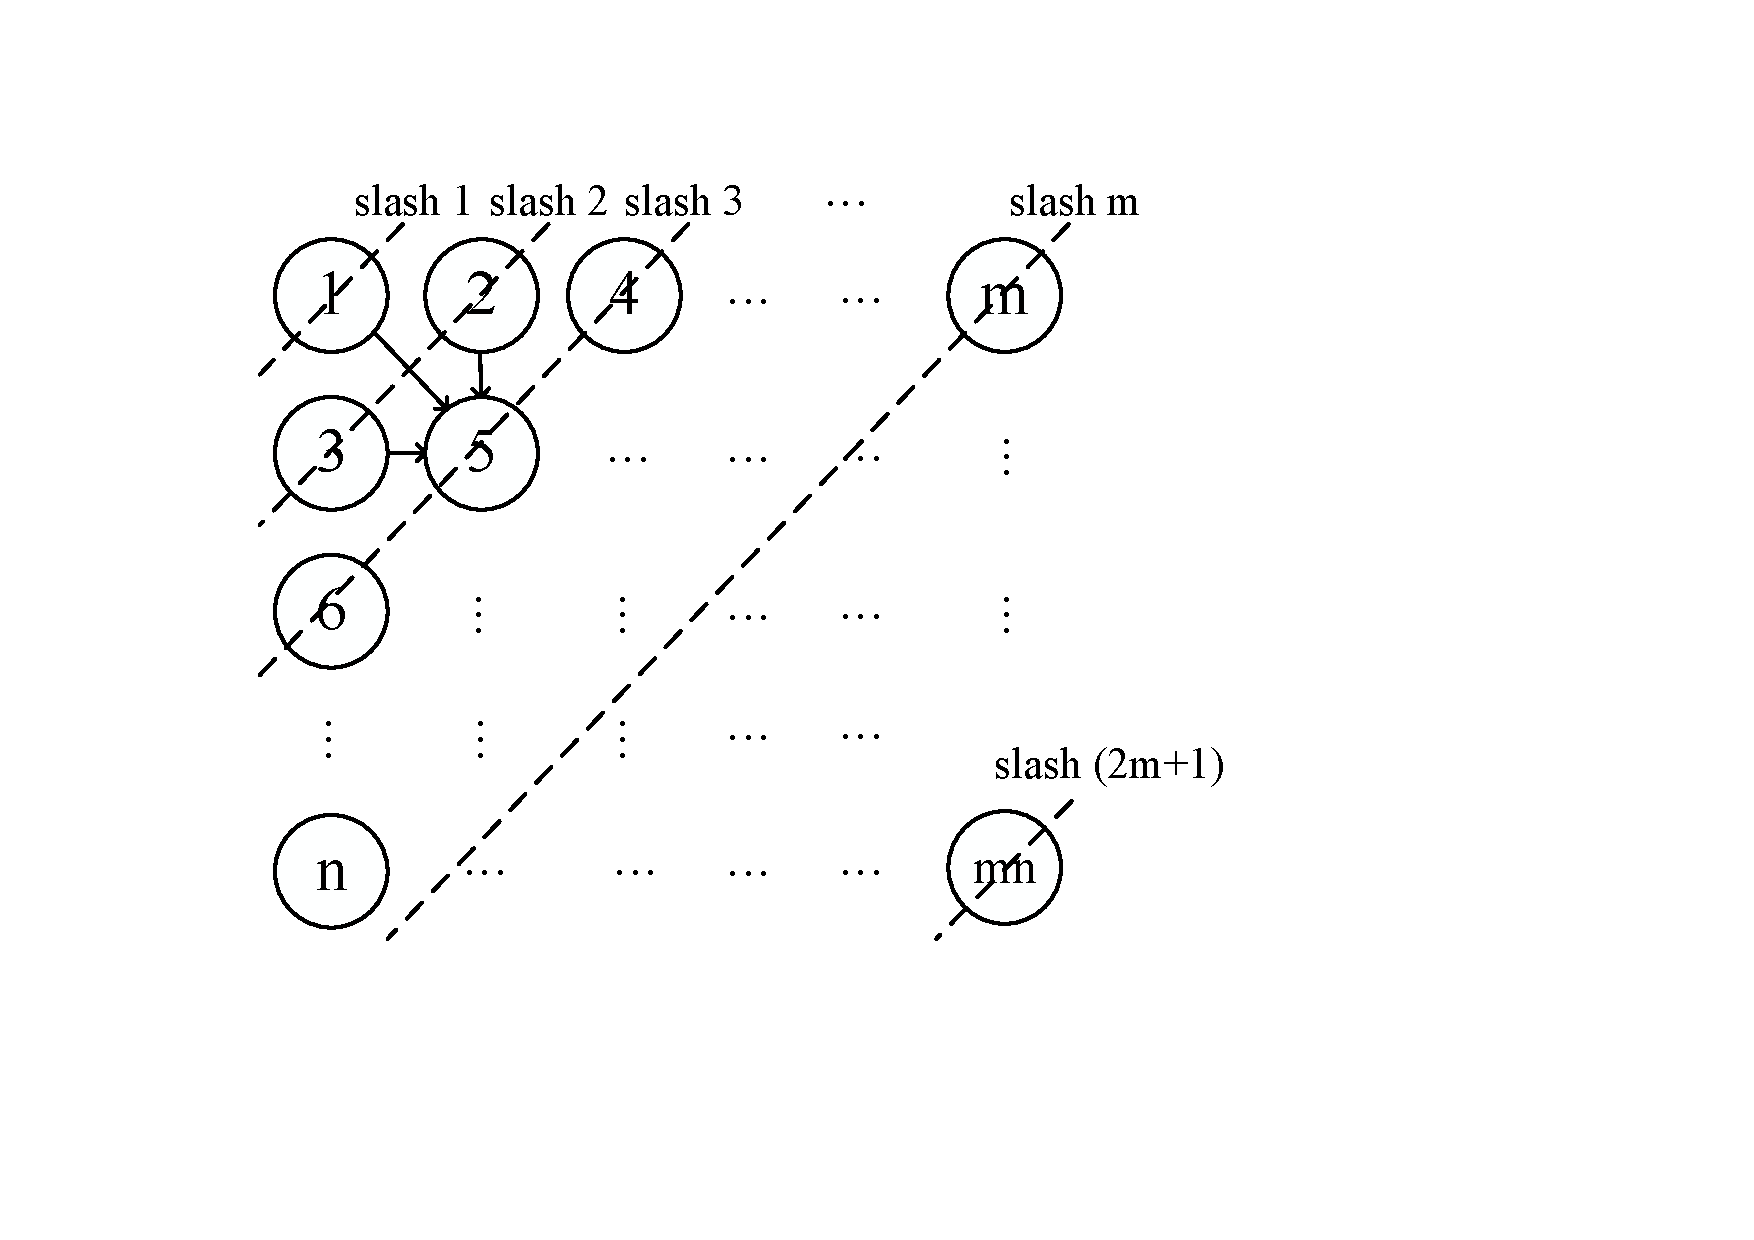
\includegraphics[width=0.48\linewidth]{pdf/DPstate.pdf}
			\caption{An example of EDR calculation procedure\label{fig:DPstate}}
		\end{figure}
	}
	
	\begin{figure}[t]
		\centering
		\scriptsize{
			\begin{minipage}{0.34\linewidth}
				\centering
				\includegraphics[width=\linewidth]{pdf/StateMatrixDP_V2.pdf}
				(a) Relationship between states on different slashes 
			\end{minipage}
			\hfill
			\begin{minipage}{0.62\linewidth}
				\centering
				\includegraphics[width=\linewidth]{pdf/EDR_fetch.pdf}
				(b) Location of data each thread reads and writes
			\end{minipage}
		}
		\caption{An example of EDR calculation procedure\label{fig:EDR}}
	\end{figure}
	
	To solve this problem, we analyse the data dependency of original calculation procedure, finding that if we group the states on the same slash together in state matrix, the value of every state only relies on the states of the last two slashes, and meanwhile the calculations of states in the same slash are independent. Figure \ref{fig:EDR}(a) shows an example. When we calculate the states 7, 8, 9 and 10 on slash 4, only the states 4, 5, 6 on slash 3 and states 2, 3 on slash 2 are needed. 
	
	Based on this observation, we propose an iterative procedure of the parallel EDR calculation in each CUDA block. For a task that $|traj_{d}|=m$ and $|traj_q|=n$, an $(m+1)\times (n+1)$-sized state matrix is maintained. In $i$-th iteration, thread $th_j$ calculate the $j$-th state on slash $i$ based on the corresponding states on slash $i-1$ and slash $i-2$. To achieve a coalesce access pattern, we store state matrix $S$ with xxx order (the order shows in figure \ref{fig:EDR}(b)), because based on this origanization values that threads read and write in each iteration are nearby. For example, on 4-th iteration, the read and write requests of threads 0-3 are continuous, contributing to the coalesce access pattern. For slashes which there are thousands of states on them, states are computed by all threads in some loops. Although not all CUDA threads work in iterations before calculating states on slash $N_{core}$, we argue that they have a small propotion of all iterations, because trajectories usually are longer than 200 meaning that there are usually more than 400 iterations in total, while $N_{core}$ is 64 or 128 on most of GPU. Therefore, a reasonble load balance is achieved in our iterative procedure.

%\begin{algorithm}[t]
%	\algsetup{linenosize=\tiny}
%	\scriptsize
%	\caption{Parallel EDR Calculation}
%	\label{alg:EDR}
%	\begin{algorithmic}[1]
%		\REQUIRE ~~\\
%		Two sets of trajectories: $\mathbb{T}_D,\mathbb{T}_Q$; Tasks information $Cand_q$; Threshold of EDR: $\epsilon$; Number of threads in a CUDA block $N_{thread}$
%		\ENSURE ~~\\
%		All EDR distance between trajectories in two sets: $EDR(T_{q},T_{d})$, $\forall (T_{q},T_{d})\in \{Cand_q|\forall q\in Q\}$
%		
%		\STATE Assign each $(T_d,T_q)$ pair to a thread block
%		\STATE Initial an array to store results of all pairs assigned: $result[size(Cand_q)]$
%		\FOR{CUDA block $bID$ \textbf{parallelly}}
%		\STATE Initial matrix $S$ in global memory: $S[len(T_q)+1][len(T_d)+1]$
%		\STATE $maxLen \leftarrow max(len(T_q),len(T_d))$
%		\STATE Load trajectories in local memory: $Tq[len(T_q)]$, $Td[len(T_d)]$
%		\STATE $slashNum \leftarrow len(T_q)+len(T_d)+1$
%		\STATE $loopPerThread \leftarrow \lceil maxLen/N_{thread}\rceil$
%		\FOR{slash $i$ from 1 to $slashNum$}
%		\FOR{thread $tID$ \textbf{parallelly}}
%		\STATE $sl_1 \leftarrow getSlashOffset(i-1)$
%		\STATE $sl_2 \leftarrow getSlashOffset(i-2)$
%		\FOR{each loop $j$ from 0 to $loopPerThread-1$}
%		\STATE $sID\leftarrow j*threadNum+tID$
%		\STATE $s_1 \leftarrow getUpState(sl_1,tID,j)$
%		\STATE $s_2 \leftarrow getLeftState(sl_1,tID,j)$
%		\STATE $s_3 \leftarrow getCrossState(sl_2,tID,j)$
%		\STATE $subCost\leftarrow geneSubCost(Tq,Td,\epsilon)$
%		\STATE $tempState[loopPerThread]\leftarrow min(s_1,s_2,s_3+subCost)$ 
%		\ENDFOR
%		\ENDFOR
%		\FOR{each thread $tID$ \textbf{parallelly}}
%		\FOR{each loop $j$ from 0 to $loopPerThread-1$}
%		\STATE $sl_{now}\leftarrow getSlashOffset(i)$
%		\STATE $sl_{now}[N_{thread}*j+tID]\leftarrow tempState[j]$
%		\ENDFOR
%		\ENDFOR
%		\ENDFOR
%		\STATE $EDR(T_q,T_d)\leftarrow S[len(T_q+1)][len(T_d+1)]$
%		\ENDFOR
%		\RETURN $EDR(\mathbb{T}_d,\mathbb{T}_q)$
%	\end{algorithmic}
%\end{algorithm}
}
\eat{
	We designed an iterative framework for parallel EDR calculation. According to the defination of EDR which is given in defination~\ref{def:edr}, the process of EDR calculation can be divided into several independent steps. Figure \ref{fig:DPstate} shows an example of calculating the EDR between two trajectorie $traj_q$ and $traj_d$ with length $m$ and $n$. Each value in a state (represented as $state[i][j]$) is calculated by comparing and choosing the minimun value of $\{state[i-1][j]+1,state[i][j-1]+1,state[i-1][j-1]+subcost\}$. After all the states have been calculated, the $state[m][n]$ is the EDR between two trajectories. If we use slashes to group the states, we notice that the values of states in one slash rely on the value of states in two upper left slashes. For example, in figure \ref{fig:DPstate}, if we want to calculate the states on slash 3, the states on slash 1 and slash 2 are needed. Meanwhile, comparing operations within a slash have no relationship, inspiring us to invoke the calculations within the same slash in parallel, forming the basic idea of our solution.
	
	\begin{algorithm}[t]
		\algsetup{linenosize=\tiny}
		\scriptsize
		\caption{Parallel EDR Calculation}
		\label{alg:EDR}
		\begin{algorithmic}[1]
			\REQUIRE ~~\\
			Two sets of trajectories: $\mathbb{T}_D,\mathbb{T}_Q$; Tasks information $Cand_q$; Threshold of EDR: $\epsilon$; parameters  $\epsilon$, $N_{thread}$
			\ENSURE ~~\\
			all EDR distance between trajectories in two sets: $EDR(T_{q},T_{d})$, $\forall (T_{q},T_{d})\in \{Cand_q|\forall q\in Q\}$
			
			\STATE assign each $(T_d,T_q)$ pair to a thread block
			\STATE initial an array to store results of all pairs assigned: $result[size(Cand_q)]$
			\FOR{each CUDA block $bID$ \textbf{parallelly}}
			\STATE initial matrix $S$ in global memory: $S[len(T_q)+1][len(T_d)+1]$
			\STATE $maxLength \leftarrow max(len(T_q),len(T_d))$
			\STATE load trajectories in local memory: $Tq[len(T_q)]$, $Td[len(T_d)]$
			\STATE $slashNum \leftarrow len(T_q)+len(T_d)+1$
			\STATE $loopPerThread \leftarrow \lceil maxLength/threadNum\rceil$
			\FOR{each slash $i$ from 1 to $slashNum$}
			\FOR{each thread $tID$ \textbf{parallelly}}
			\STATE initial an array in GPU SM's register to store states calculated: $tempState[loopPerThread]$
			\FOR{each loop $j$ from 0 to $loopPerThread-1$}
			\STATE update $tempState[j*threadNum+tID]$ using states on last two slashes
			\ENDFOR
			\ENDFOR
			\FOR{each thread $tID$ \textbf{parallelly}}
			\FOR{each loop $j$, $j\in [0,loopPerThread-1]$}
			\STATE flush $lastTwoSlash[0][j*threadNum+tID]$ to $state$ in corresponding position
			\STATE $lastTwoSlash[0][j*threadNum+tID]\leftarrow lastTwoSlash[1][j*threadNum+tID]$
			\STATE update $lastTwoSlash[1][j*threadNum+tID]$ using $tempState[j]$
			\ENDFOR
			\ENDFOR
			\ENDFOR
			\STATE $result[bID]\leftarrow state[len(t_1)][len(t_2)]$
			\ENDFOR
		\end{algorithmic}
	\end{algorithm}
	
	Based on this framework, we propose a procedure of calculating EDRs in parallel on GPU, as algorithm \ref{alg:EDR} shows, whose implement is based on CUDA. Given a set of EDR calculation tasks, we first assign each of them to a block to make GPU full-loading, in order to improve the throughtput(line 1-2). In each block, the values of states are calculated in $(2\times max\{m,n\}+1)$ loops from $state[0][0]$ to $state[m][n]$ slash by slash (line 10). For example, in figure \ref{fig:DPstate}, state on slash 1 is generated, and then slash 2, slash 3, ..., until the slash $(2m+1)$. In each loop data on two before slashes are stored in high-speed local memory of each SM, which is allocated before starting loops (line 6), because they will be frequently accessed by threads. Noting that the length of trajectory is almost smaller than 2048, it is enough for space of local memory to store these data. As for the state matrix of this calculation, we store them according to the order of slash, as figure \ref{fig:DPstate} shows. In this case, the data required by threads are nearby, assuring the coalesce accessing pattern.
	
	
	
	
	
	In each thread block, based on the data of previous two slashes, all the values on current slash are calculated by mass of threads in parallel by equation (1) mentioned in Section II (line 11-16). After finishing the calculation on current slash i, the states on slash i-2 stored in local memory are flushed into state matrix in global memory, and then states on slash i-1 and i become the new "two last slashes" (line 17-22). The result of EDR calculation of this block can be extracted from state matrix after all loops (line 25). 
	
	We can see that in our solution, the number of steps needed for EDR?calculation reduces from $mn$ to $(2max\{m,n\}+1)$ comparing to not using GPU, and this reduction could be so obvious if trajectory length $m$ or $n$ is large, which is usually an actual situation because the sample interval of location device is short, e.g. 2s.
	
	% In each loop, states in two before slashes are stored as shared variables because in CUDA programming model all shared variables will be stored in high speed local memory and calculation of states on slash $i$ is related to states on slash $(i-1)$ and $(i-2)$. In this way all of states accessing transactions required from EDR calculation are from high speed local memory. In addition to this, we find that calculation of $state[i][j]$ needs for $traj_1[i]$ and $traj_2[j]$ and in some loops all of trajectory points are required. Also storing them as shared variables is surely a choice. However, for limited capabacity of local memory, this choice will impact the efficiency of GPU. This is because in GPU architecture, each SM can execute at most 8 blocks therotically at a time but all of shared variables of blocks are needed to be resident in local memory. So abusement of shared variables may limit the number of blocks running on an SM at the same time. For this reason, we choose 
	
	\begin{algorithm}[t]
		\algsetup{linenosize=\tiny}
		\scriptsize
		\caption{Parallel EDR Calculation}
		\label{alg:EDR}
		\begin{algorithmic}[1]
			\REQUIRE ~~\\
			Two sets of trajectories: $T1,T2$
			
			Threshold of EDR: $\epsilon$
			
			Parallel parameters: $blockNum$, $threadNum$
			\ENSURE ~~\\
			all EDR distance between trajectories in two sets: $EDR(t_{1},t_{2})$, $\forall (t_{1},t_{2})\in T1\times T2$
			
			\STATE assign each $(t_1,t_2)$ pair to a thread block
			\STATE initial an array to store results of all pairs assigned: $result[blockNum]$
			\FOR{each block $bID$ \textbf{parallelly}}
			\STATE initial a matrix in global memory to store all states: $state[len(t_1)+1][len(t_2)+1]$
			\STATE $maxLength \leftarrow max(len(t_1),len(t_2))$
			\STATE initial a matrix in local memory to store states in last two slashes: $lastTwoSlash[2][maxLength+1]$
			\STATE $lastTwoSlash[0][0]=0$
			\STATE $slashNum \leftarrow len(t_1)+len(t_2)-1$
			\STATE $loopPerThread \leftarrow \lceil maxLength/threadNum\rceil$
			\FOR{each slash $i$, $i\in [1,slashNum]$}
			\FOR{each thread $tID$ \textbf{parallelly}}
			\STATE initial an array in GPU SM's register to store states calculated: $tempState[loopPerThread]$
			\FOR{each loop $j$, $j\in [0,loopPerThread-1]$}
			\STATE update $tempState[j*threadNum+tID]$ using states on last two slashes
			\ENDFOR
			\ENDFOR
			\FOR{each thread $tID$ \textbf{parallelly}}
			\FOR{each loop $j$, $j\in [0,loopPerThread-1]$}
			\STATE flush $lastTwoSlash[0][j*threadNum+tID]$ to $state$ in corresponding position
			\STATE $lastTwoSlash[0][j*threadNum+tID]\leftarrow lastTwoSlash[1][j*threadNum+tID]$
			\STATE update $lastTwoSlash[1][j*threadNum+tID]$ using $tempState[j]$
			\ENDFOR
			\ENDFOR
			\ENDFOR
			\STATE $result[bID]\leftarrow state[len(t_1)][len(t_2)]$
			\ENDFOR
		\end{algorithmic}
	\end{algorithm}
	
	
	%% ??????kernel?????????????????GPU????
	%% ??????kernel?????????????????GPU????
	%% ??????kernel?????????????????GPU????
	We propose a multi-GPU implementation of our strategy dealing with large-scale of EDR calculation from all top-k trajectory queries by dividing the set of EDR calculation tasks into several equal size part, to achieve a load balancing and maximum usage of multiple GPUs. Before running these tasks, we use an independent memory allocated table (MAT) to store trajectory data when they are loaded into GPU global memory first, because in this way if a trajectory has been loaded into global memory, by looking for MAT we can avoid the duplicated low-speed data transfering between memory and GPU. However, the volume of the GPU global memory is usually so limited that not all trajectory data can be filled into it. To make an tradeoff, we maintain a memory pool and integrate it to MAT. If the pool is full, we use Least Recently Used (LRU) algorithm to drop some outdated trajectories. This strategy is efficient in real life because there exists hotspot within queries. For example, trajectories in city center may be required by queries more frequently because the population in city center is denser than rural area. After the kernel finishing, EDR calculation results from different GPUs are collected and query engine then filters the candidates, as shown in line 9 in algorithm \ref{alg:TSQ_1}.
}


\section{Experimental Evaluation}\label{sec:exp}
%In this section, we conduct experiments based on two real trajectory datasets to verify the performance of \frname.

\subsection{Experiment Setup}

\noindent \textbf{Datasets.}
We use two real-life trajectory datasets: SHCAR and  GeoLife~\cite{DBLP:journals/debu/ZhengXM10}. 
SHCAR contains trajectories of 9,446 private cars in Shanghai, China, collected from 2014 to 2015. GeoLife contains trajectories from 182 users during Apr. 2007 -- Aug. 2012, where most trajectory points are within Beijing, China.
%
%\noindent \textbf{Preprocessing.}
The original datasets contain one complete trajectory for each user. 
We split the sequence of trajectory points from each user into several subsequences, to obtain trajectories for $\alltraj$. If two consecutive points have more than 30 minutes timestamp gap, we split them into two raw trajectories.
%we seem the sequence of sample points of a the same user as a  trajectory. If the difference between two time stamps of consecutive  points in a trajectory is larger than 30 minutes, we call this point a  ``gap''. We then split the trajectory into several new trajectories  according to these gaps.
%This is because trajectories with these gaps are usually not  meaningful single route, which we usually do not concern about.
%By this preprocessing all raw trajectories are the routes of a single  trip.
%For example, the point sequence of a single car may includes sample  points of the trips from home to office and from office to home, and  after spliting two trajectories showing two trips respectively can be  generated.
Table~\ref{tab:datasets} provides the details of two datasets.
\begin{table}[t]
	% increase table row spacing, adjust to taste
	\renewcommand{\arraystretch}{1.1}
	
	% if using array.sty, it might be a good idea to tweak the value of
	% \extrarowheight as needed to properly center the text within the  cells
	\caption{Statistics of datasets}\label{tab:datasets}
	\centering
	% Some packages, such as MDW tools, offer better commands for making  tables
	% than the plain LaTeX2e tabular which is used here.
	{\small
		\begin{tabular}{|c|c|c|c|c|}
			\hline
			& \#Traj. & avg. traj. length & \#Points & \#Cells\\
			\hline
			SHCAR & 327,474 & 848 & 75,188,293& 262,144\\
			\hline
			GeoLife & 30,325 & 926.4 & 19,143,208& 262,144\\
			\hline
		\end{tabular}
	}
\end{table}


\noindent \textbf{Baselines.}
For range query, we compare \frname with its CPU version, and two GPU approaches: STIG~\cite{7498315} and FSG~\cite{GPUTaxi}. 
%As they are designed for high-dimensional points rather than trajectories, we seem range query as extracting $tid$ of points which are within given range $R$.
%we only evaluate range query processing on the sample points in trajectories for these two baselines. 
%We also implement our approach on multicore CPU as a baseline method.

\noindent $\bullet$ \textbf{STIG~\cite{7498315}.} This approach leverages \emph{kd-tree}~\cite{DBLP:journals/cacm/Bentley75}, where the leaf nodes correspond to blocks of points.
We keep kd-tree in memory and use CPU to compute candidate blocks, which will be refined by GPU to get final result.
%, in which each leaf node corresponds to a data block rather than a point. 
%We choose in-memory CPU-GPU hybrid strategy of it, which means kd-tree is firstly traversed by CPU and some candidate blocks are returned, then each block is refined by GPU in parallel.

\noindent $\bullet$ \textbf{FSG~\cite{GPUTaxi}.} This approach uses a flat grid-file based index to accelerate point-in-polygon queries over taxi trip data. Similar to our approach, it first find cells which overlap query region, then generate candidate cell-polygon pairs and send them to GPU for parallel verification.

\noindent $\bullet$ \textbf{\frname-CPU-R.} This is the CPU version of \frname using multi-threading, where each candidate block is assigned to a thread running on CPU for verification. 
%All the parameters are set the same as that of \frname.

To the best of our knowledge, we are the first to exploit GPU to accelerate top-$k$ similarity query using EDR as the distance function. Hence, we only compare \frname with its CPU version with multi-threading. 
%, we only implement a CPU-based method EDR-MCPU, which is the origin~\cite{DBLP:conf/sigmod/ChenOO05} of our approach, as the baseline of the implementation on multicore CPU. 

\noindent $\bullet$ \textbf{\frname-CPU-S.} This is the CPU-version of \frname, which adapts histogram sequential scan~\cite{DBLP:conf/sigmod/ChenOO05} to multi-threaded processing.
%The parameters of this method are set the same as that in our approach.

\noindent \textbf{Metrics.}
We measure the performance of the approaches by the total execution time over a batch of queries. For indexing cost, we measure the construction time and memory cost. 
%We also use speedup ratio compared to the CPU baseline with single thread to measure the acceleration of \frname.

We run all the experiments on a server equipped with two 10-core Xeon E5-2650 v3 processor clocked at 2.3GHz, 64GB of RAM, 4TB of disk storage and a two-chip NVIDIA Tesla K80 GPU. Each chip has 2,496 CUDA cores and 12GB graphical memory. We implemented \frname in C++ with CUDA 8.0, running on CentOS 7. We conduct our experiments under various parameter settings. Table~\ref{table_param} shows the meaning and range of all parameters, where default values are underlined. All the results are averaged over 10 runs.
%Unless otherwise specified, we use the default values.

%\noindent \textbf{Parameters.}~~We conduct our experiment under various parameter settings. Table \ref{table_param} shows the range and default value of all parameters. The parameters are divided into two kinds: (1) query parameters, which act as the condition of trajectory query; (2) system parameters, which reflect the configuration of our framework. When testing query parameters 

\begin{table}[!t]
	% increase table row spacing, adjust to taste
	\renewcommand{\arraystretch}{1.1}
	
	% if using array.sty, it might be a good idea to tweak the value of
	% \extrarowheight as needed to properly center the text within the cells
	\caption{Parameters ranges and default values}
	\label{table_param}
	\centering
	% Some packages, such as MDW tools, offer better commands for making tables
	% than the plain LaTeX2e tabular which is used here.
	{\scriptsize
		\begin{tabular}{|c|l|l|}
			\hline
			Parameter & Description & Range\\
			\hline
			$n$ & \tabincell{l}{Max quadtree level} & $7$, $8$, $\underline{9}$, $10$ \\
			\hline
			$\theta_p$ & \tabincell{l}{Block size threshold} & \tabincell{l}{$200$, $2000$, $\underline{20000}$, $200000$} \\
			\hline
			$S_{R}$ & Query region area ($km^2$) & \tabincell{l}{$0.002$, $\underline{0.004}$, $0.006$, $0.008$} \\
			\hline
			$k$ & \tabincell{l}{Top $k$ for similarity query} & $5$, $10$, $15$, $\underline{20}$, $25$\\
			\hline
			$\zeta$ & \tabincell{l}{Avg. query trajectory length} & \tabincell{l}{$200$, $400$, $600$, $\underline{800}$, $1000$} \\
			\hline
			$N_{\rangeq}$ & \tabincell{l}{\#range queries} & \tabincell{l}{$40$, $60$, $\underline{80}$, $100$, $120$}\\
			\hline
			$N_{\simq}$ & \tabincell{l}{\#similarity queries}& \tabincell{l}{$20$, $\underline{40}$, $60$, $80$, $100$}\\
			\hline
			%shenyy: where is data size?
		\end{tabular}
	}
\end{table}


%\subsubsection{Experiment Overview} ???All other parameters are tuned to the optimal case.
%
%After that, the scalability is tested. As there is no method to shut some cores in GPU, we can only test the situation with different number of GPUs.
%
%In query performance part, same as the most of previous works, we use query latency as our metric. We compare the query time latency of two kinds of queries in different baselines and state-of-the-art systems in a large query set situation. When testing range query, we randomly generate range queries with different areas and positions and reckon the time consumption during finishing all of queries. To reflect the true working environment as much as possible, the chosen positions are restricted to the central district of Shanghai ($31.11^{\circ} N-31.36^{\circ} N, 121.39^{\circ} E-121.58^{\circ} E$). For similarity query, some trajectories are selected randomly from dataset as the query set. During the query, for each trajectory in query set, the result of top-$k$ similarity query is returned under the settings of different query parameters including $k$ and $\epsilon$. Queries are handled with formed query set and time consumption in both baseline method and GTS are then calculated. 



\subsection{Comparison of Various Approaches}

%In this section we compare the throughput of our approach with the baseline methods.
% mentioned before in range query and top-$k$ similarity query. 
%Execution time under different number of queries in a batch on two datasets is measured as the metric of throughput.

\begin{figure}[!t]
	\centering
	\scriptsize{
		\begin{minipage}{0.48\linewidth}
			\centering
			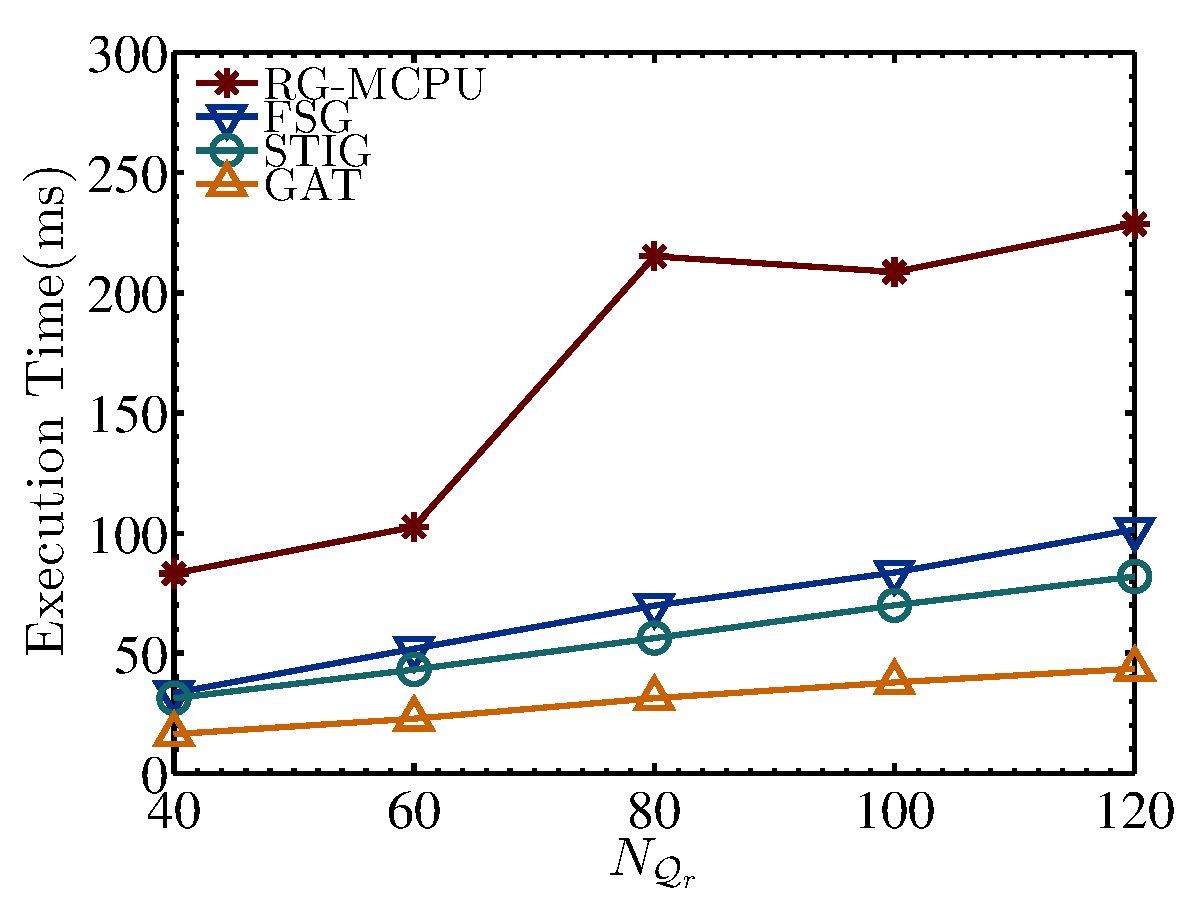
\includegraphics[width=\linewidth]{eps/QueryNum_RangeQ.eps}
			(a) SHCAR
		\end{minipage}
		\hfill
		\begin{minipage}{0.48\linewidth}
			\centering
			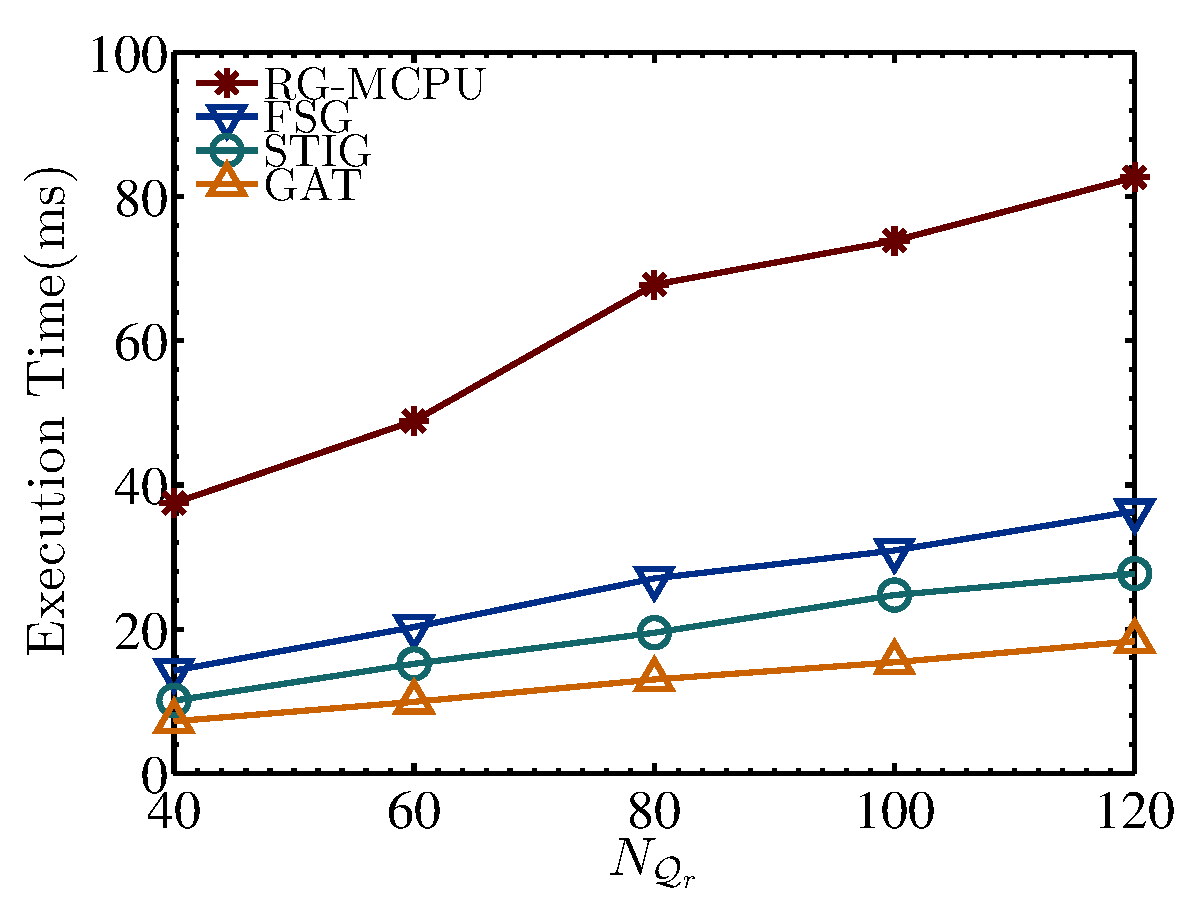
\includegraphics[width=\linewidth]{eps/QueryNum_RangeQ_GEO.eps}
			(a) GeoLife
		\end{minipage}	
	}
	\caption{Range query results\label{fig:QueryNum_range}}
\end{figure}

\begin{figure}[!t]\centering
	\scriptsize{
		\begin{minipage}{0.48\linewidth}
			\centering
			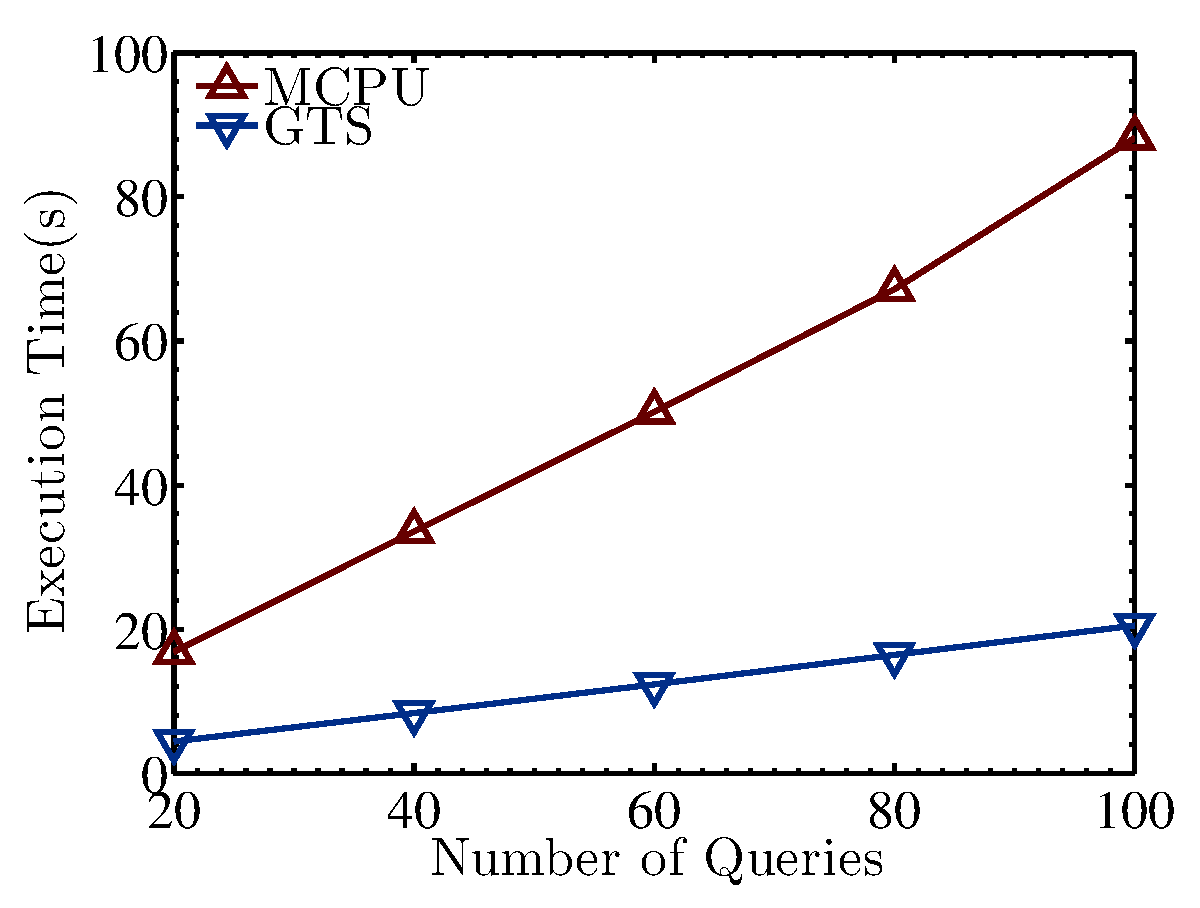
\includegraphics[width=\linewidth]{eps/QueryNum_SimilarityQ.eps}
			(b) SHCAR
		\end{minipage}
		\hfill
		\begin{minipage}{0.48\linewidth}
			\centering
			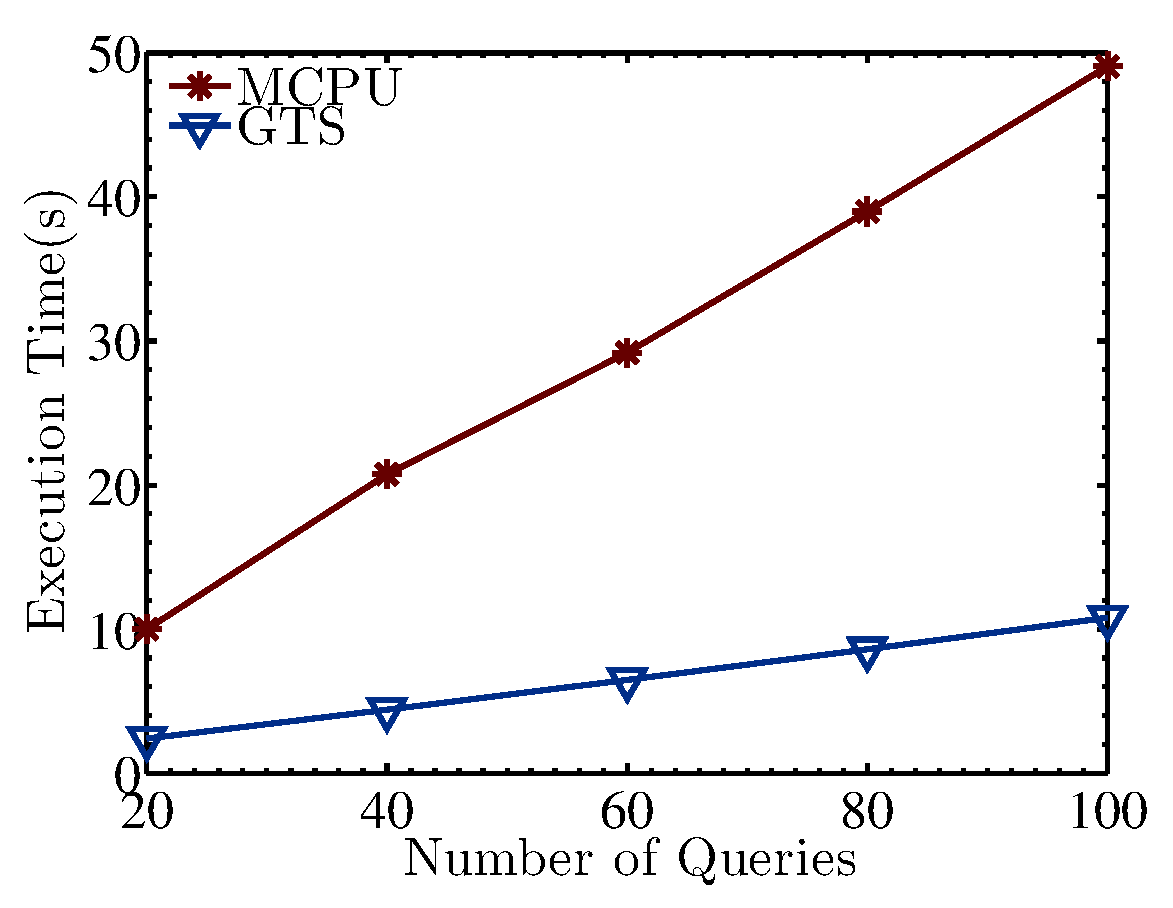
\includegraphics[width=\linewidth]{eps/QueryNum_SimilarityQ_GEO.eps}
			(b) GeoLife
		\end{minipage}
	}
	\caption{Similarity query results\label{fig:QueryNum_sim}}
\end{figure}

\noindent \textbf{Range Query.}
Figure~\ref{fig:QueryNum_range}(a) and Figure~\ref{fig:QueryNum_range}(b) show the execution time with different number of range queries on SHCAR and Geolife, respectively. The execution time in all approaches increases when the number of queries becomes larger.
Our approach outperforms the other three baselines over all cases and the advantage becomes more significant with more queries. 
%The execution time of \frname increases sub-linearly with the number of queries, thanks to the high parallelism from GPU.
On average, \frname runs 128\% and 89\% faster than FSG and STIG, respectively. We observe that GAT requires lower data transfer cost due to the memory allocation table, while the cost in FSG and STIG is relatively high. 
STIG performs better than FSG. This is because STIG uses a kd-tree like index to ensure similar number of trajectory points among blocks, leading to more balanced workload. This benefit is also achieved by \frname. \frname-CPU-R requires the longest execution time in all cases due to the limited parallelism in multi-core settings.
%shenyy: check
%In \frname hundreds of queries can be finished within $50$ ms, which meet the requirement of real-time service.

\noindent \textbf{Similarity Query.}
Figure~\ref{fig:QueryNum_sim}(a) and Figure~\ref{fig:QueryNum_sim}(b) shows the execution time with different number of similarity queries on SHCAR and Geolife, respectively. \frname runs faster than \frname-CPU-S over all the query numbers, which indicates its high throughput using GPU.
However, the number of GPU cores used by \frname is 100 larger than that of CPU cores used by \frname-CPU-S, which is mainly caused by the difference of frequency between CPU and GPU cores, the cost of data transferring on PCIe, and the execution time of calculating FDs and generating candidates included in total execution time.
%shenyy: why 5 times?? you used 20 cpu cores?but 2000 gpu cores!!explain this
On two datasets, the execution time of \frname and \frname-CPU-S increases linearly with the number of queries. Both approaches require longer execution time on SHCAR as it contains more trajectories.

%Two methods both show a linear increment in time consumption with the scale of queries. 
%We can see that \frname approach we proposed outperforms EDR-MCPU under all $N_\rangeq$
%%, and as the increasing number of queries, the gap of the performance between these two methods becomes larger.
%The result shows that the GPU-based acceleration of EDR calculation, which is the main source of the computational cost in top-$k$ similarity query, improves the throughput significantly. 

%\begin{figure}[!t]\centering
%	\includegraphics[width=8cm]{pdf/SpeedUp.pdf}
%	\caption{Speedup ratio of both range query and top-k similarity query on one GPU and two GPUs respectively, compared to the single-core CPU implementation\label{fig:SpeedUp}}
%\end{figure}





\subsection{Indexing Cost}

\begin{figure}[!t]\centering
	\scriptsize{
		\begin{minipage}{0.48\linewidth}
			\centering
			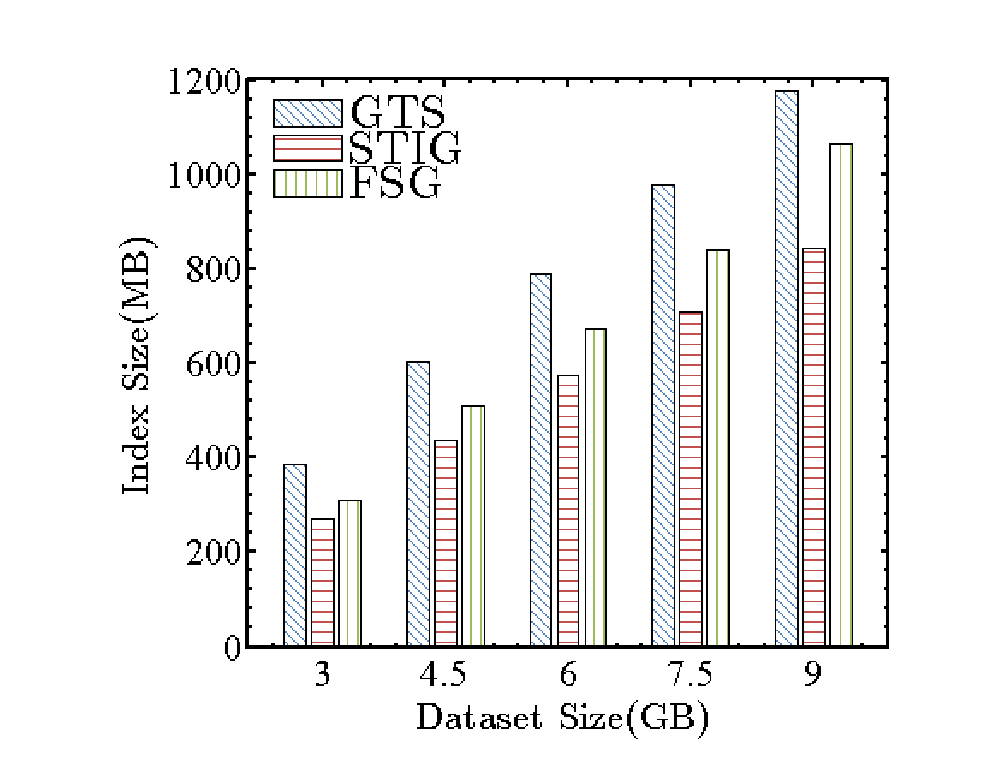
\includegraphics[width=\linewidth]{eps/indexSize.eps}
			(a) Memory Occupation
		\end{minipage}
		\hfill
		\begin{minipage}{0.48\linewidth}
			\centering
			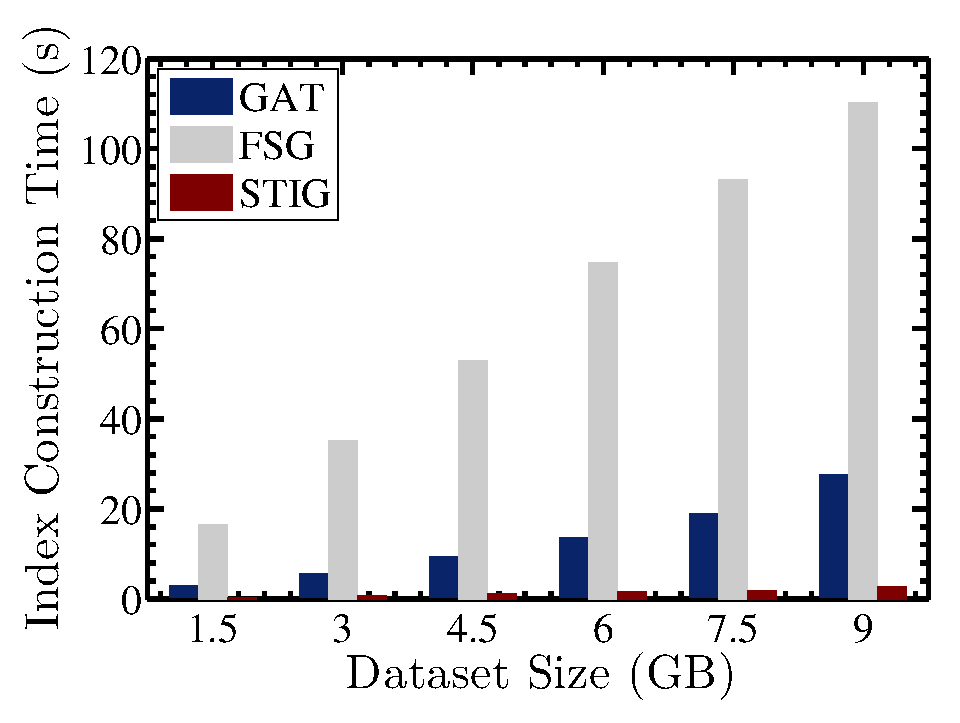
\includegraphics[width=\linewidth]{eps/indexTime.eps}
			(b) Indexing Building Time
		\end{minipage}
	}
	\caption{Indexing Cost\label{fig:IndexCost}}
\end{figure}

We evaluate indexing cost for three GPU approaches. We randomly select subsets of trajectories from SHCAR and GeoLife, and build indices for each subset.
% The result are shown in Figure~\ref{fig:IndexCost}. 
%All the parameters are set to default. 

\noindent \textbf{Memory Cost.}
Figure~\ref{fig:IndexCost}(a) shows the index memory cost w.r.t. different data sizes.
For all the approaches, the size of indices becomes larger when the data size increases. 
There is a small increment ($8$-$29$\%) of memory cost in \frname compared to other two methods. The main reason is that \frname involves trajectory index to reconstruct trajectories and apply histogram-based pruning for similarity queries, while STIG and FSG can only processing range queries and do not maintain such indices. 
On average, the overhead of \idxname is merely $12.8$\% of the data size, which is acceptable and space-efficient.
%In the evaluation of $9$GB dataset only about $80$MB to $290$MB more memory is consumed compared to FSG ($1063$MB) and STIG ($853$MB), it is an acceptable cost considering the big increment on throughput in \frname.

\noindent \textbf{Index Construction Time.}
Figure \ref{fig:IndexCost}(b) provides index construction time over different data sizes. 
The cost increases as the data size becomes large. For 9GB data size, \frname takes only $27.7$ second for index construction, which indicates time efficiency. 
\frname requires $75.2$\% less index construction time than STIG over all the data sizes. This is because STIG needs to compute a large number of medium values when generating kd-tree. 
The index construction time of \frname is more than FSG due to the additional tree index $\treeindex$ in \frname.

\subsection{Speedup}
We now study the speedup achieved by \frname under default parameters with one and two GPUs. For comparison, we use a single thread to execute all the queries on CPU. All the speedups are computed as the ratios of execution time against the single-thread approach.
%This study explains two benefits. First, it shows that our GPU-based implementation can outperform traditional implementation on CPU. Second, it demonstrates that a near-linear improvement of efficiency can be achieved by adding more GPU devices.
Table \ref{tab:speedup} shows the speedups for two kinds of queries over two datasets.
%
For range queries, \frname with 1 GPU achieves $20.07$ and $18.03$ speedups over SHCAR and GeoLife respectively, owning to the high parallelism of GPU. Using 2 GPUs achieves about $1.76$x speedup than using 1 GPU over both datasets. This indicates that \frname can speedup nearly linearly with more GPU cores.
%
For similarity queries, \frname with 1 GPU achieves $35.54$ and $38.94$ speedups over SHCAR and GeoLife, respectively. The speedups are higher than those for range queries. Compared with similarity queries, range query processing involves simple comparison operations and the data transfer cost between main memory and global memory may become more significant in the overall execution time, which restricts the increase of speedup.

%Our approach achieves up to $38.94$ speedup in evaluation of top-$k$ similarity query for single GPU, and 74.95x in dual GPUs environment. The high speedup ratio comes from the parallel execution of compute-intensive EDR calculation. 
%For range query, a lower speedup ratio of 20.07x for single GPU and 37.63x for dual GPUs is achieved. Considering that only some comparison operations need to be performed in varification procedure, the larger propotion of data transfering cost restricts the speedup ratio compared to similarity query.


\begin{table}[t]
	\centering
	
	\caption{Speedup achieved in two datasets}     % NOTE!  caption goes _before_ the table contents !!
	\label{tab:speedup}
	
	\begin{small}
		\begin{tabular}{|l|c|c|c|c|}
			\hline
			{\bfseries Dataset} & \multicolumn{2} {c|} {\bfseries SHCAR} & \multicolumn{2} {c|} {\bfseries GeoLife} \\
			\cline{1-5}
			{\bfseries \#GPUs} & {\bfseries 1GPU} &  {\bfseries 2GPU}  & {\bfseries 1GPU} &  {\bfseries 2GPU}  \\
			\hline
			Range Query & 20.07 & 37.63 & 18.03 & 32.43 \\
			\hline
			Top-k Similarity Query & 35.54 & 68.53 & 38.94 & 74.95 \\
			\hline
		\end{tabular}
	\end{small} 
\end{table}



\subsection{Scalability}

%Figure~\ref{fig:Scalability} presents the results under different size of data in the range from $3$GB to $9$GB.

\begin{figure}[t]\centering
	\scriptsize{
		\begin{minipage}{0.48\linewidth}
			\centering
			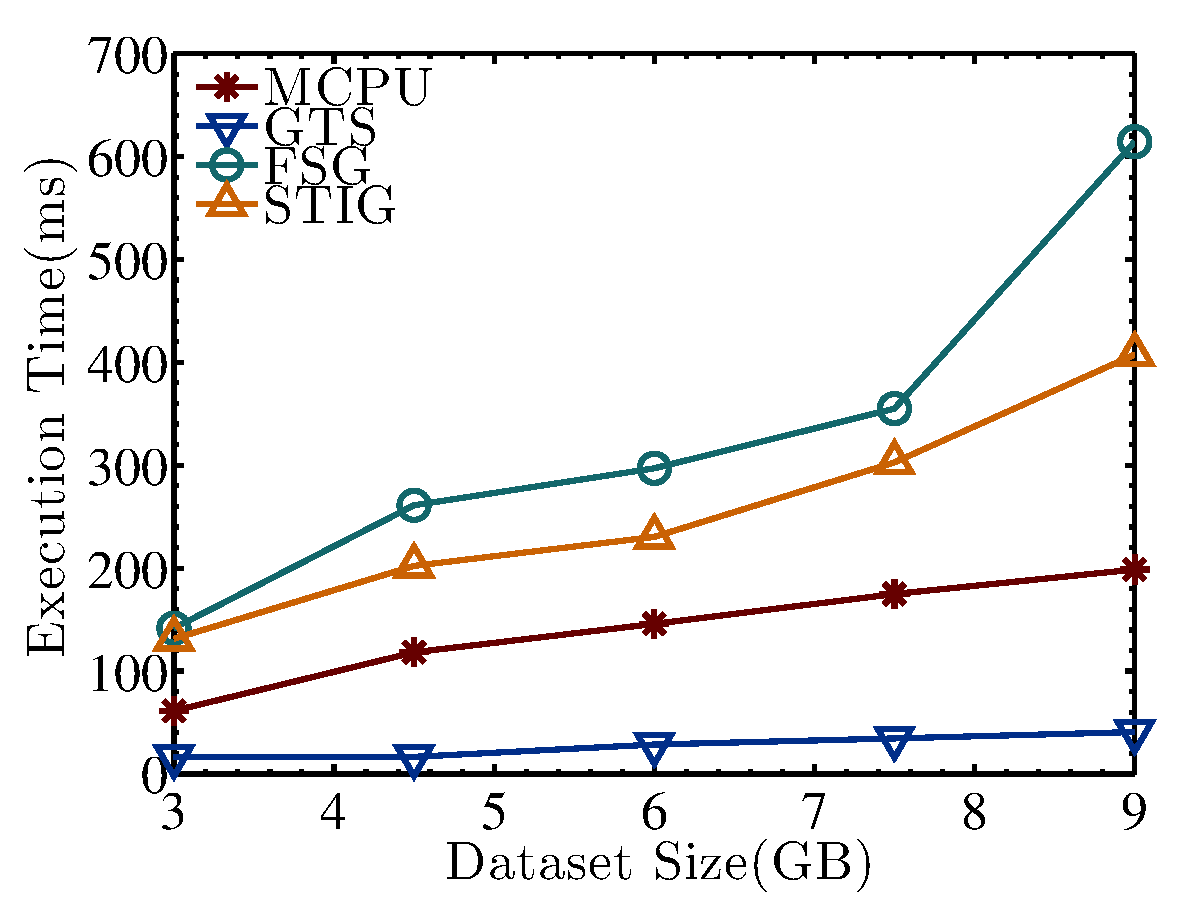
\includegraphics[width=\linewidth]{eps/range_scala.eps}
			(a) Range Query
		\end{minipage}
		\hfill
		\begin{minipage}{0.48\linewidth}
			\centering
			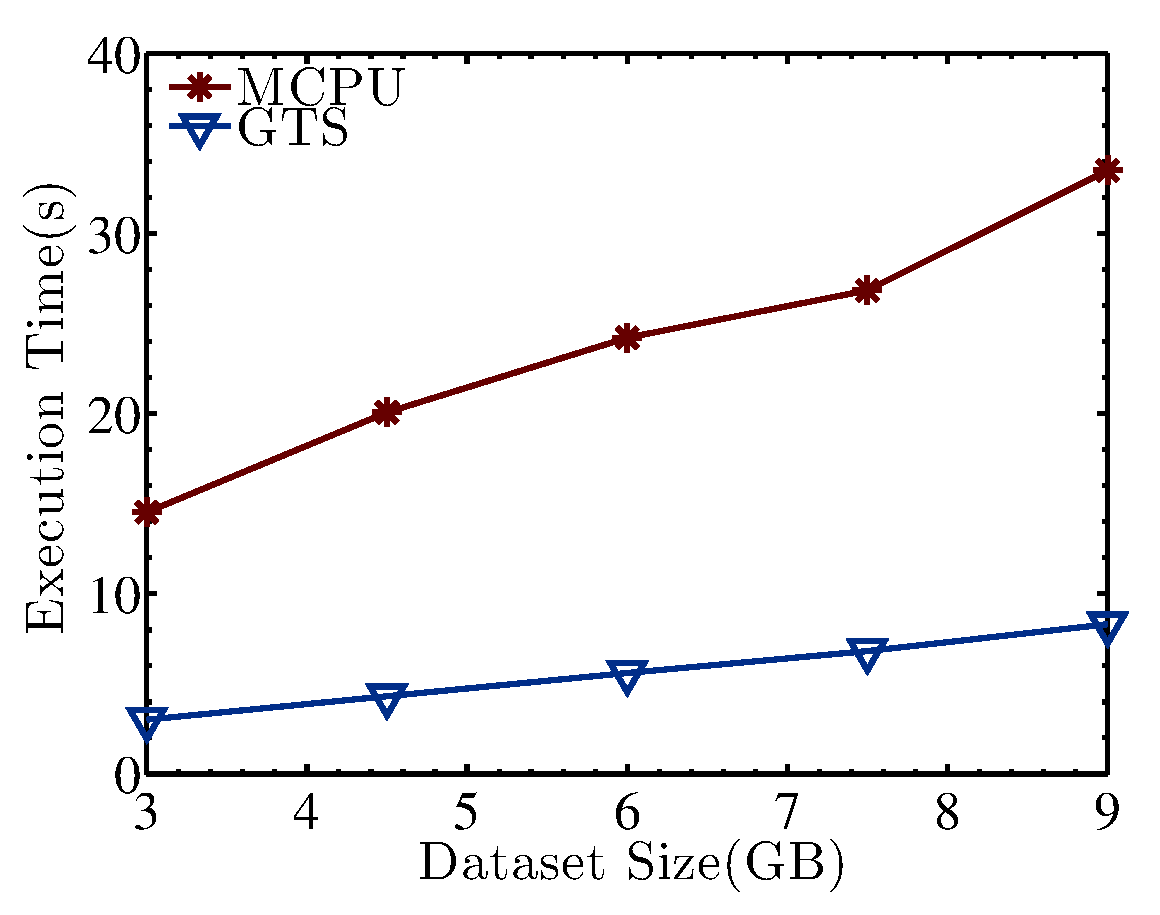
\includegraphics[width=\linewidth]{eps/similarity_scala.eps}
			(b) Similarity Query
		\end{minipage}
	}
	\caption{Scalability\label{fig:Scalability}}
\end{figure}

We investigate the scalability of different approaches, by varying the data size from $3$GB to $9$GB.
%\noindent \textbf{Range Query.}
Figure~\ref{fig:Scalability}(a) shows the execution time of 80 range queries over different data sizes. All the approaches require longer execution time when the dataset becomes larger. This is determined by the fact that more candidates are included for verification over larger datasets.
\frname scales better than FSG, because in \frname the effect of the skew dataset is mitigated owing to the quadtree-like index in \idxname, while FSG suffers from unbalanced workloads on different GPU cores caused by different number of points in each cell of flat grid-file based index. This phenomenon is more significant on larger dataset, which limits the scalability of FSG.
%shenyy: fillin
%
%However, as the growing scale of dataset, the execution time on GPU-based methods show a sub-linear increasing trend. This is because the increment of more expensive data transferring between main memory and GPU is quicker than that of quantity of candidates waiting for verification.\textbf{Why?????????}
%We can also see our approach performs better when facing large scale dataset than other GPU-based baselines, indicating that our system has a good scalability on range query. 
%
%\noindent \textbf{Similarity Query.}
The execution time of similarity queries over different data sizes is shown in Figure~\ref{fig:Scalability}(b). We can see as the data volume grows, both \frname and \frname-CPU-S require longer execution time. However, the execution time of \frname grows much slower than that of \frname-CPU-S, indicating better scalability using GPU.
% two approaches consume more time on queries and the benefit of acceleration by using GPU becomes more obvious. It also proves that our system works excellently on large-scale dataset.


\subsection{Parameter Tuning}

In this section, we study the effects of different parameter values on the performance of \frname, as listed in Table~\ref{table_param}. 
%Some of them can be categorized as query parameters, which are properties of queries and can be evaluated in both other systems and GTS, such as the area of MBR and $k$. Others are system parameters, which only exist in our system. For this reason, we show results of all baselines when evaluating the execution time in different query conditions to demonstrate both the expected performance in various environment and the effects of these parameters. Meanwhile, system parameters are evaluated under different query scales to show the effects, which are only based on our approach. 

%\noindent \textbf{Range Query.}~~There are three parameters about range query: $S_R$, $\theta_p$ and $n$. We will evaluate the effects of them.

\begin{figure}[!t]\centering
	\scriptsize{
		\begin{minipage}{0.48\linewidth}
			\centering
			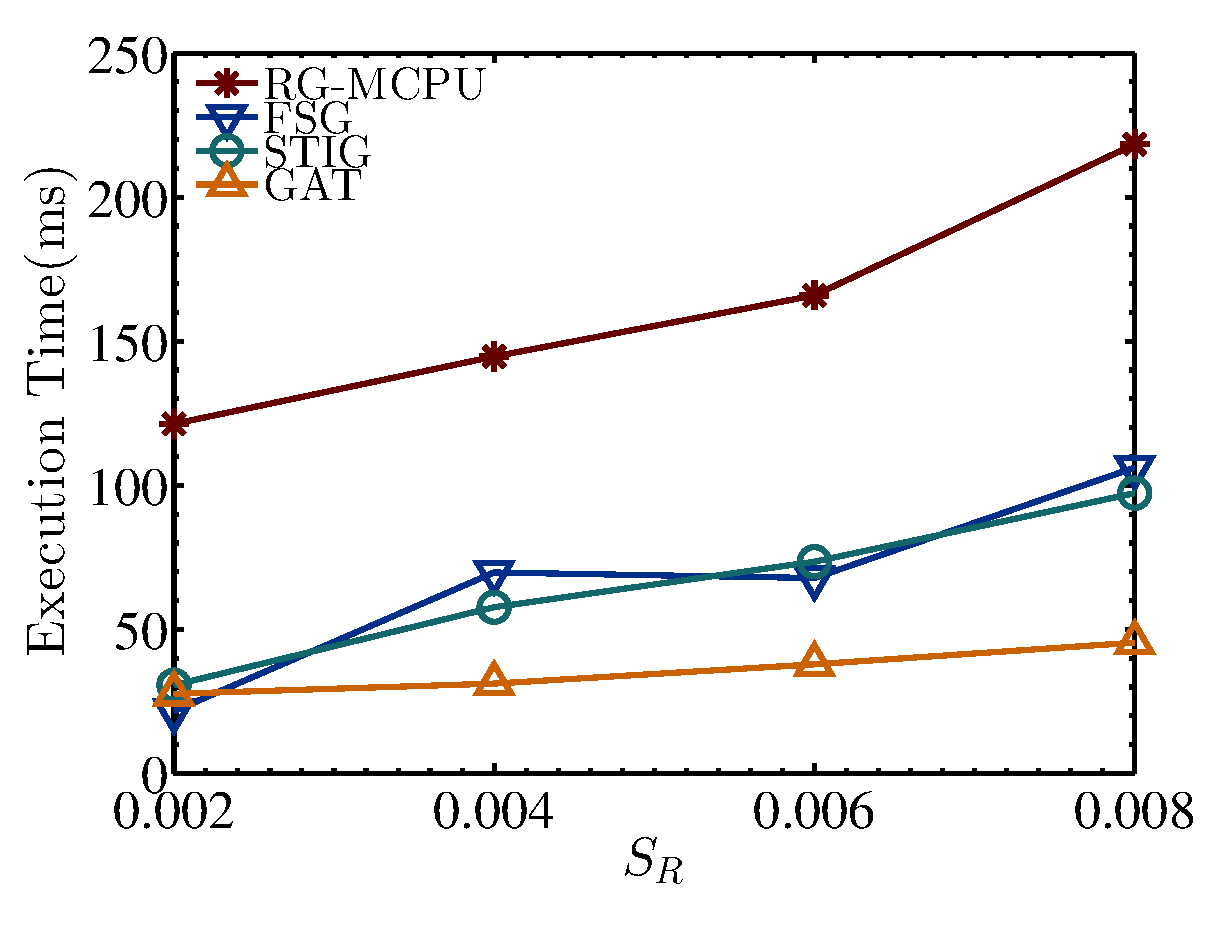
\includegraphics[width=\linewidth]{eps/RangeArea.eps}
			(a) SHCAR
		\end{minipage}
		\hfill
		\begin{minipage}{0.48\linewidth}
			\centering
			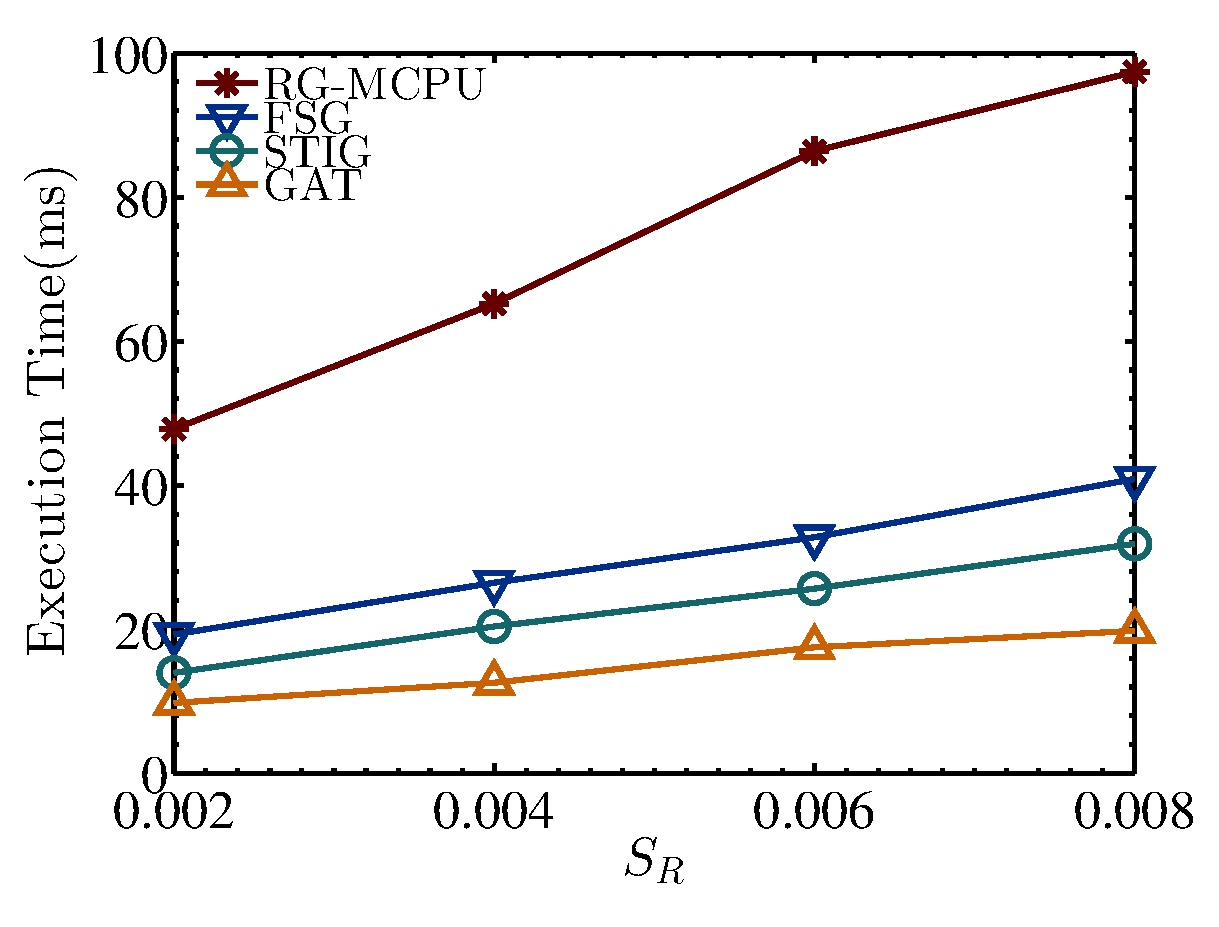
\includegraphics[width=\linewidth]{eps/RangeArea_GEO.eps}
			(b) GeoLife
		\end{minipage}
	}
	\caption{Effects of query region area ($R_{\rangeq}$) \label{fig:RANGE}}
\end{figure}

% zbw: in this part the unit of area can be transfromed into standard unit
\noindent \textbf{Effect of query region area $S_R$ ($km^2$).}
The area of query region $S_{R}$ controls the selectivity of range query. All the query regions are generated by extending from a point in the city center. Figure~\ref{fig:RANGE} shows the results of queries with different $S_{R}$.
The execution time of all approaches increases as the area of $R$ varies from $0.002$ to $0.008$. 
%shenyy: show unit in figures.
As the query region becomes larger, more blocks will be overlapped with $R$, leading to more candidates for verification.
\frname performs the best over all the areas on GeoLife dataset, but runs slightly slower than FSG for $S_R=0.002$. The reason may be that in the query on SHCAR with a small $S_R$, only one or two cells in a block are overlapped with $R$, but in \frname all points covered by any cells in this block need to be verified by GPU. However in FSG only points in cells which overlapped $R$ need to be checked whether they are within $R$. 
%On average, \frname runs $?$x and $?$x faster than STIG and FSG, respectively. 
All GPU solutions outperform \frname-CPU-R in all cases, due to the superior of GPU in parallel computation.

%We can see that this trend is nearly linear for our framework, because the scale of verification and the number of nodes overlapped by query region $R$ are basically propotional to the area of it. 
%Our frameworks shows a better throughput even in the query region with a large area. 


\begin{figure}[t]\centering
	\scriptsize{
		\begin{minipage}{0.48\linewidth}
			\centering
			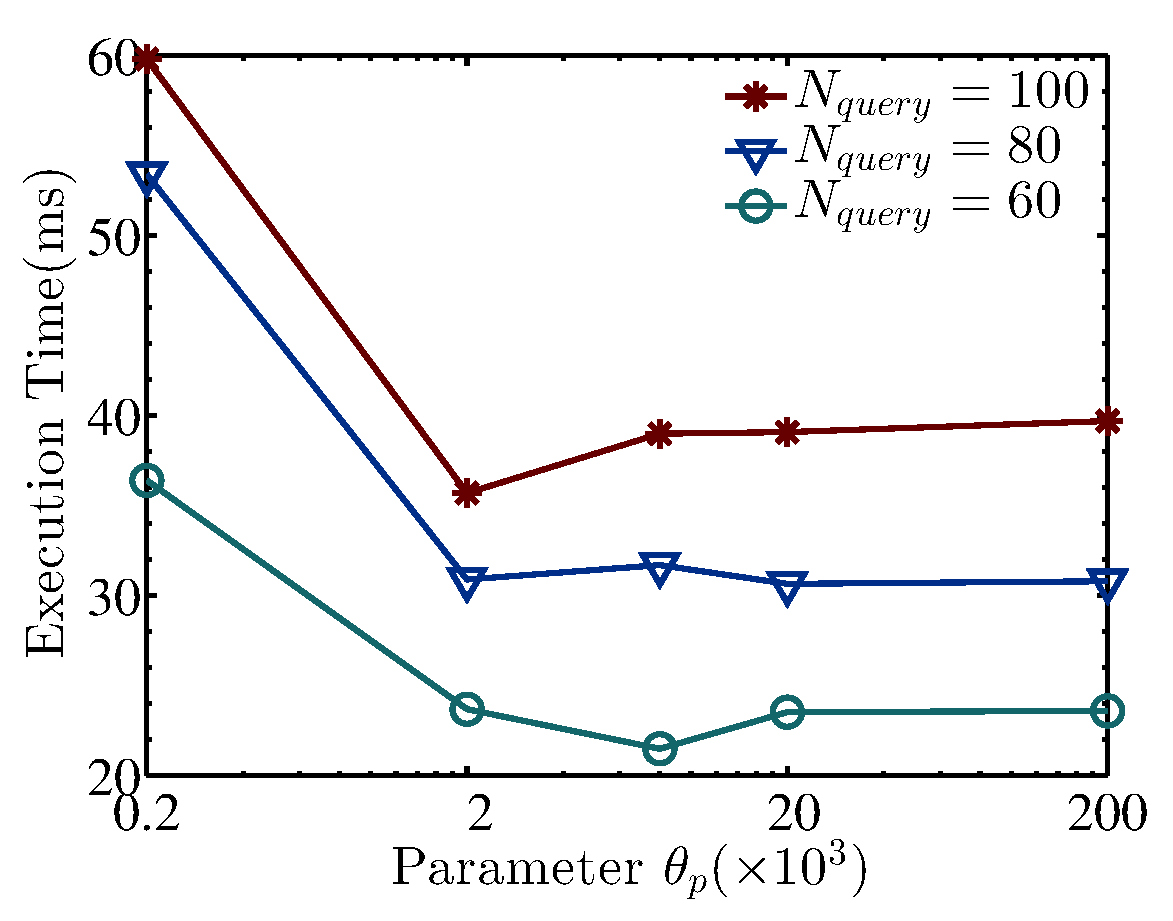
\includegraphics[width=\linewidth]{eps/MCELL.eps}
			(a) SHCAR
		\end{minipage}
		\hfill
		\begin{minipage}{0.48\linewidth}
			\centering
			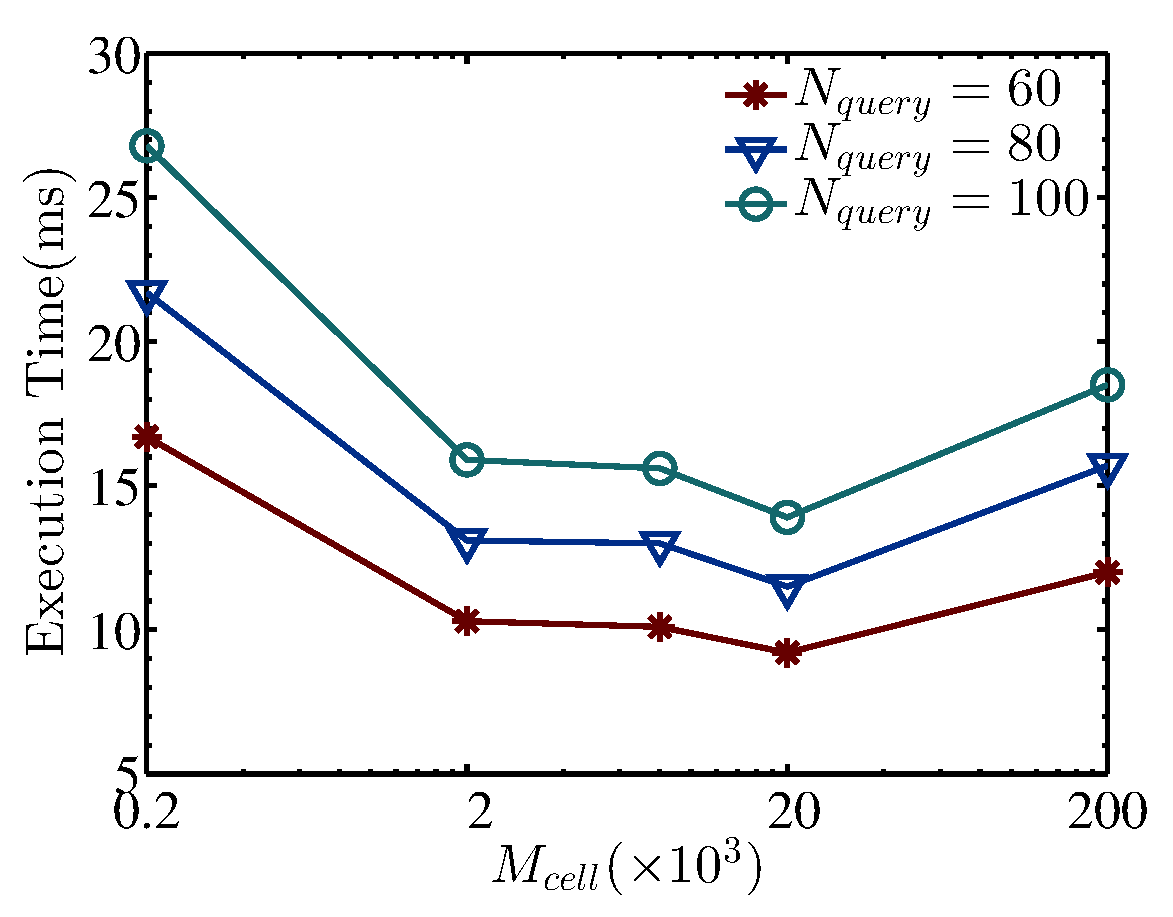
\includegraphics[width=\linewidth]{eps/MCELL_GEO.eps}
			(b) GeoLife
		\end{minipage}
	}
	\caption{Effects of maximal \#points covered by a leaf node ($\theta_p$) \label{fig:MCELL}}
\end{figure}

\noindent \textbf{Effect of block size threshold $\theta_p$.}
%shenyy: remove theta_p=8000 in the figures
Figure \ref{fig:MCELL} shows the execution time of range queries with various values of $\theta_p$. Recall that a large value of $\theta_p$ means that more points are within a block to be verified in each GPU SM, while total number of blocks is smaller.
%shenyy:explain
%of $N_{\rangeq}=60$, $N_{\rangeq}=80$ and $N_{\rangeq}=100$. 
For both datasets, we observe that the execution time of \frname decreases significantly when $\theta_p$ varies from $200$ to $2000$.
%, and then becomes stable for larger values of $\theta_p$.
When $\theta_p$ is too small, the number of leaf nodes in $\treeindex$ increases significantly and the number of points per candidate block becomes smaller. As we assign a candidate block of points to one GPU SM, verifying a small number of points in a candidate block cannot fully utilize the parallelism of GPU SM.
We also observe a slight increase in execution time when $\theta_p$ varies from $20,000$ to $200,000$. This is because larger $\theta_p$ results in more points in each candidate block and the difference in the point number per block becomes larger. Such variance causes imbalanced workloads among GPU SMs.


%We can see under about $\theta_p=8000$ and $\theta_p=20000$ our approach achieves the best performance on both datasets respectively. 
%There is a downward trend of execution time as decreasing $\theta_p$, because if $\theta_p$ is too small, each SM of GPU need only finish several comparison operations between points and the query region (e.g., less than the number of cores in SM), leading to not fully usage of GPU. 
%On the other hand, in the result of Geolife, as $\theta_p$ continues to increase from $20000$, the execution time goes up slightly. This is because the workload of verification tasks on each SM becomes extremely large, so the absolute gap among the cost of each task is indeed bigger, leading to an unbalanced workload.

\begin{figure}[!t]\centering
	\scriptsize{
		\begin{minipage}{0.48\linewidth}
			\centering
			\includegraphics[width=\linewidth]{eps/n_filter.eps}
			(a) SHCAR
		\end{minipage}
		\hfill
		\begin{minipage}{0.48\linewidth}
			\centering
			\includegraphics[width=\linewidth]{eps/n_FD.eps}
			(b) GeoLife
		\end{minipage}
	}
	\caption{Effects of maximal \#level of $\treeindex $ ($n$) \label{fig:LCELL}}
\end{figure}


\noindent \textbf{Effect of maximum quadtree level $n$.} 
$n$ controls the number of cells in $\allcell$. As we use $\theta_p$ to group cells into blocks, the performance of \frname on range queries quite stable against different values of $n$. We thus omit the results due to space limit.
Figure~\ref{fig:LCELL} provides the execution time of similarity queries on two datasets by varying the maximum quadtree level $n$. We can see as the growth of $n$, the time consumption of calculating frequency distance increases. The reason  is that the length of FVs are exponential to the parameter $n$, which is propotion to the computational cost of FD, although through implementing FV as a BST this effect has been mitigated. Execution time of the iterations between generating candidates and calculating EDR decreases as $n$ becomes larger because of a stronger pruning power from the tighter lower bound of EDR generated from fine-grained FVs.
%shenyy: use new figures!!
%Figure \ref{fig:LCELL} shows the result when parameter $n$ varying from $7$ to $10$, noting that with the restriction that $\theta_p=20000$, $n$ has to be set larger than $7$, or the number of points in some cells will exceed $20000$. 
%%We can see the there is only slight change of performance. This is because the cells are grouped into blocks during filtering phase as the unit of task assignment, so the change of the number and size of cells do not affect the task division and varification scale in each SM significantly, which are the main factors of the performance.
%In SHCAR, execution time of range queries decrease mildly as the larger $n$, because in this situation a more fine-grained division of cells are performed, then through grouping cells into blocks the number of points in each block becomes more balance. 
%However, in GeoLife, the execution time increase slightly under larger $n$. This may be because in some dense area fine-grained cells directly form the leaf nodes in level $n$ of $\treeindex$, leading to a greater depth in these branches and then more cost of filtering.

%\noindent \textbf{Similarity Query.}~~In this section, we study the effects of parameters in top-$k$ similarity query, including $k$ and $\zeta$.


\begin{figure}[!t]\centering
	\scriptsize{
		\begin{minipage}{0.48\linewidth}
			\centering
			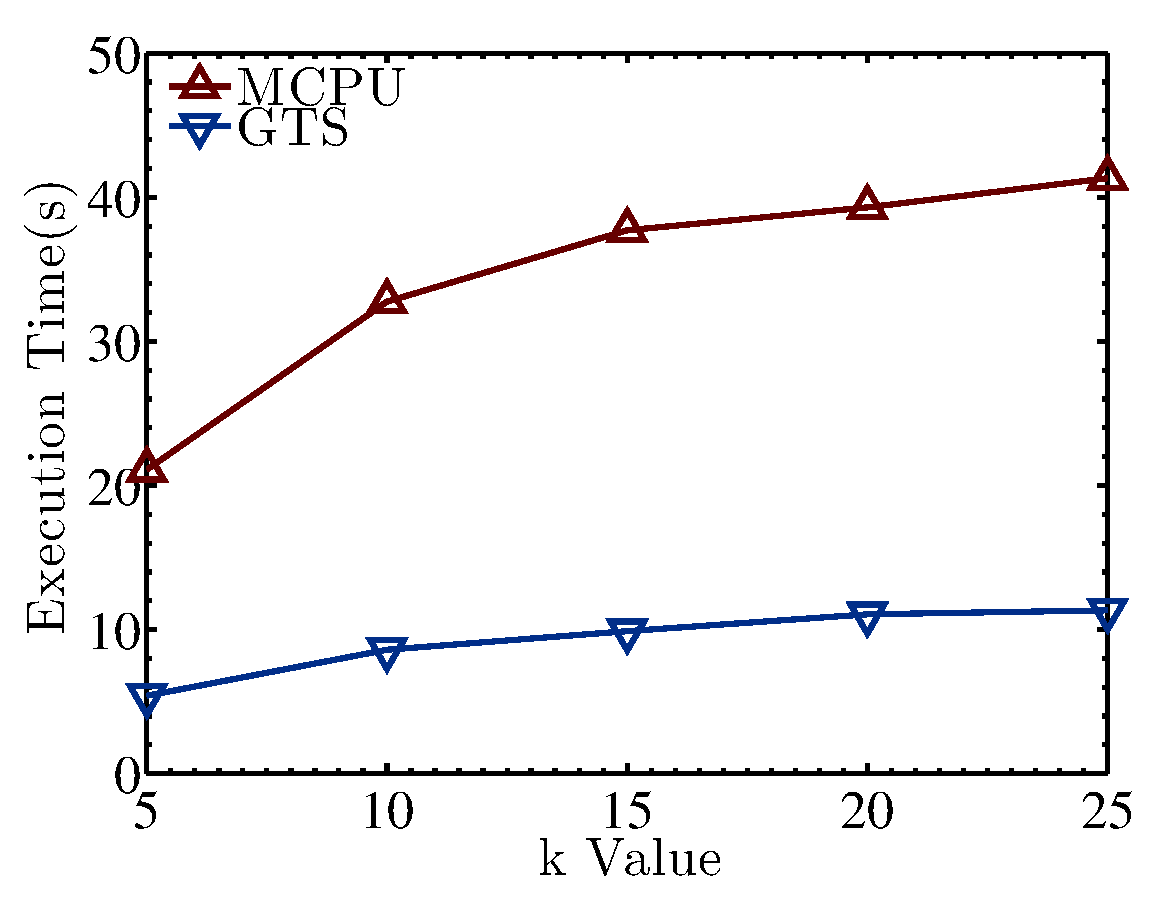
\includegraphics[width=\linewidth]{eps/kValue.eps}
			(a) SHCAR
		\end{minipage}
		\hfill
		\begin{minipage}{0.48\linewidth}
			\centering
			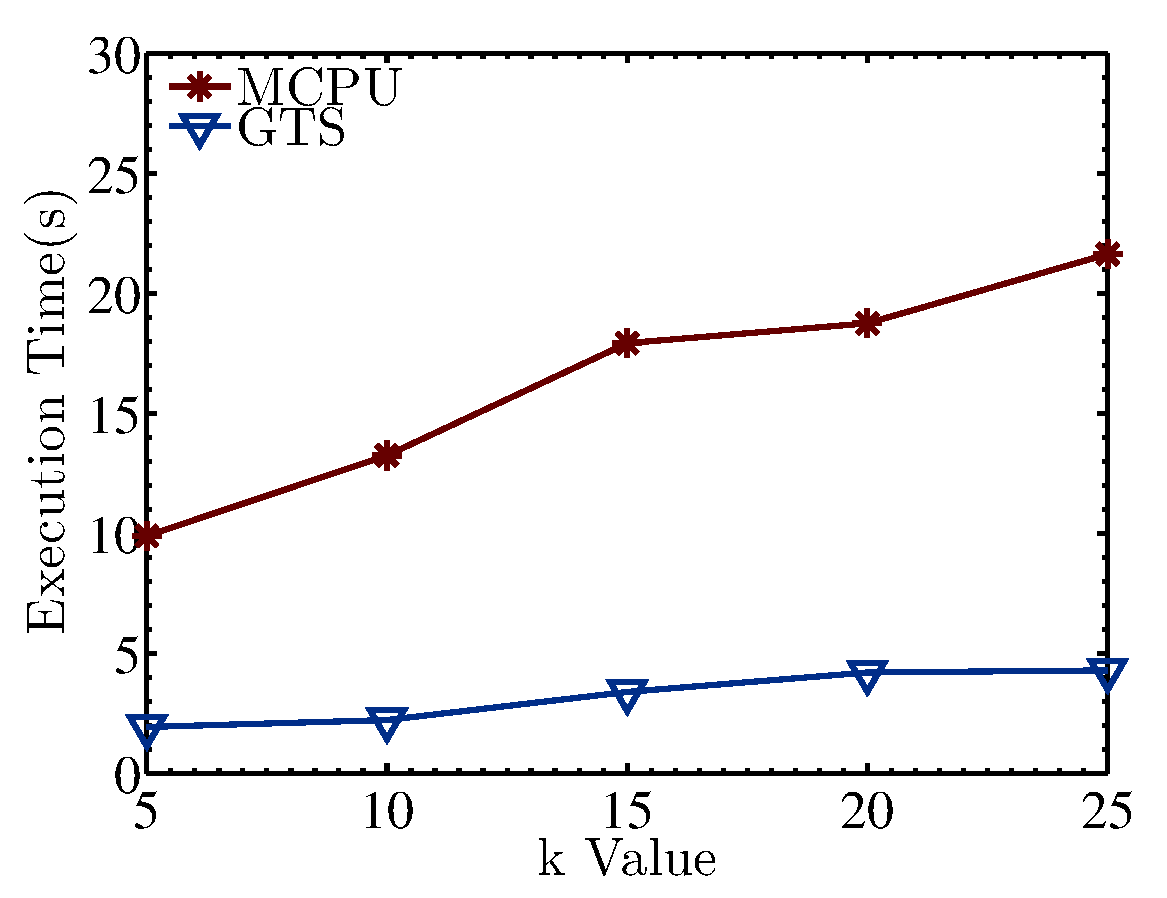
\includegraphics[width=\linewidth]{eps/kValue_GEO.eps}
			(b) GeoLife
		\end{minipage}
	}
	\caption{Effects of $k$ \label{fig:kValue}}
\end{figure}

\noindent \textbf{Effect of $k$.}
Figure~\ref{fig:kValue} shows the execution time of similarity queries under different values of $k$. As $k$ becomes larger, both \frname and \frname-CPU-S requires longer execution time. This is because larger $k$ involves more EDR distances being performed.
However, the increase in the execution time of \frname is negligible as the EDR computation task is distributed among thousands of GPU cores and the performance is even further amortized with larger $k$.


%We can see that for all $k$ values our approach achieves better performance than CPU-based implementation.
%In both two approaches, execution time goes higher as the $k$ value increases. This is because under a larger $k$ more EDR should be calculated before reaching terminate condition. The amplitude of increment in the number of EDR calculation becomes smaller as $k$ grows, so the execution time tends to be constant after $k$ is large enough. 



\begin{figure}[!t]\centering
	\scriptsize{
		\begin{minipage}{0.48\linewidth}
			\centering
			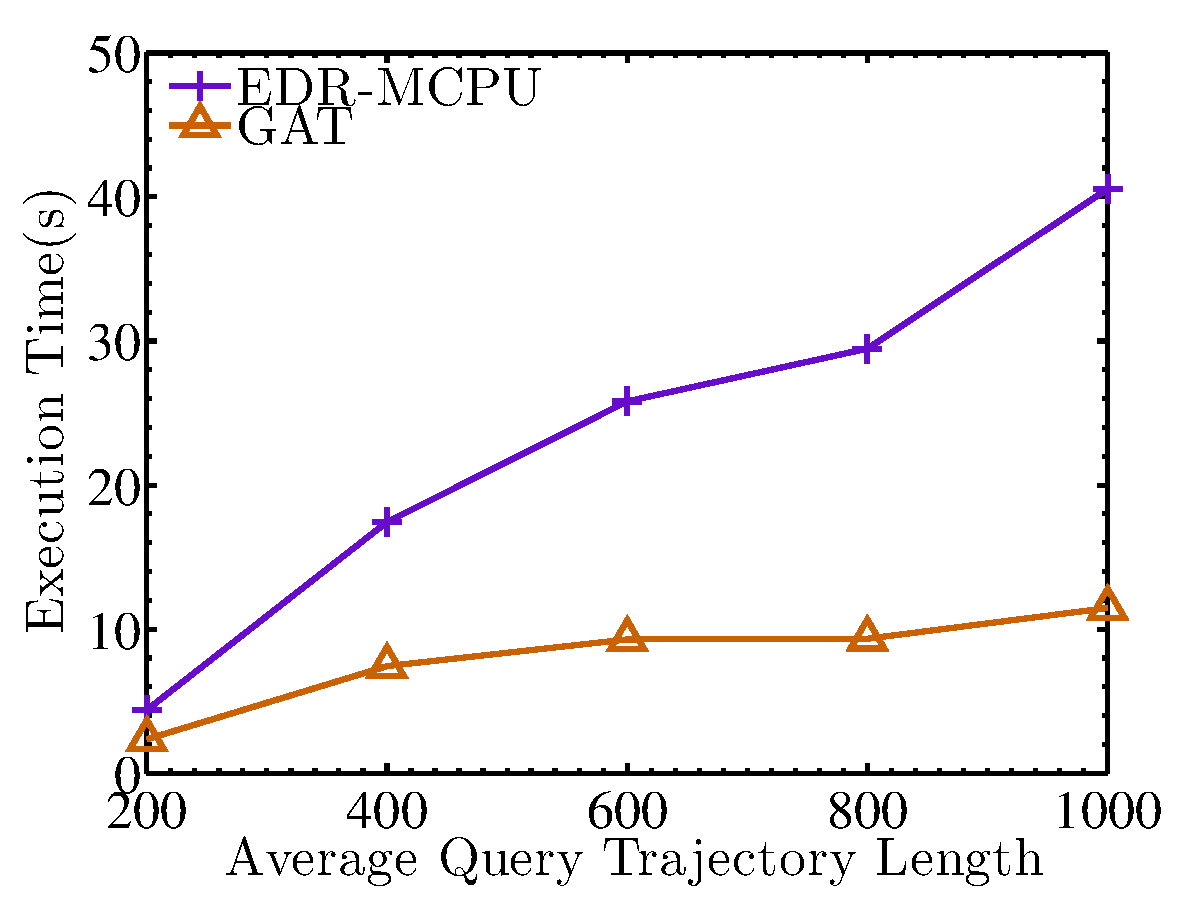
\includegraphics[width=\linewidth]{eps/QueryLength.eps}
			(a) Execution time
		\end{minipage}
		\hfill
		\begin{minipage}{0.48\linewidth}
			\centering
			\includegraphics[width=\linewidth]{eps/trajLength_GEO.eps}
			(b) Speedup ratio
		\end{minipage}
		%%shenyy: replace with a new graph
	}
	\caption{Effects of query trajectory length ($\zeta$) \label{fig:LENSIMI}}
\end{figure}

\noindent \textbf{Effect of average query trajectory length $\zeta$.}
We study the effects of average query trajectory length on similarity query processing. For each length, we randomly choose $10$ trajectories and report the averaged result.
%In each test, we choose ten different trajectories of the same length as query trajectories and reckon the execution time.
%To concern on the effects of trajectories' length, We control the factor of different FD calculation cost in by using trajectories with the same cell-based trajectory but different length to form a query set.
Figure~\ref{fig:LENSIMI} shows the execution time and speedup ratio by varying the length of query trajectories.
For both SHCAR and GeoLife, \frname outperforms \frname-CPU-S over all the trajectory lengths. The advantage of \frname becomes more significant for larger trajectories lengths. The reason is that the computational cost of EDR distance is proportional to query trajectory length and \frname computes each distance with multiple GPU cores in parallel, leading to slow increment of execution time for larger $\zeta$.

%speedup ratio rises linearly as the growing length of query trajectory, meaning that our approach can achieve a higher speedup for longer query trajectory. The reason of this phenomenon is that the cost of each EDR calculation is mainly determined by number of iteration, which is linear with the length of query trajectory.

%\noindent \textbf{Effect of $n$.}~~
%\begin{figure}[!t]\centering
%	\scriptsize{
%		\begin{minipage}{0.48\linewidth}
%			\centering
%			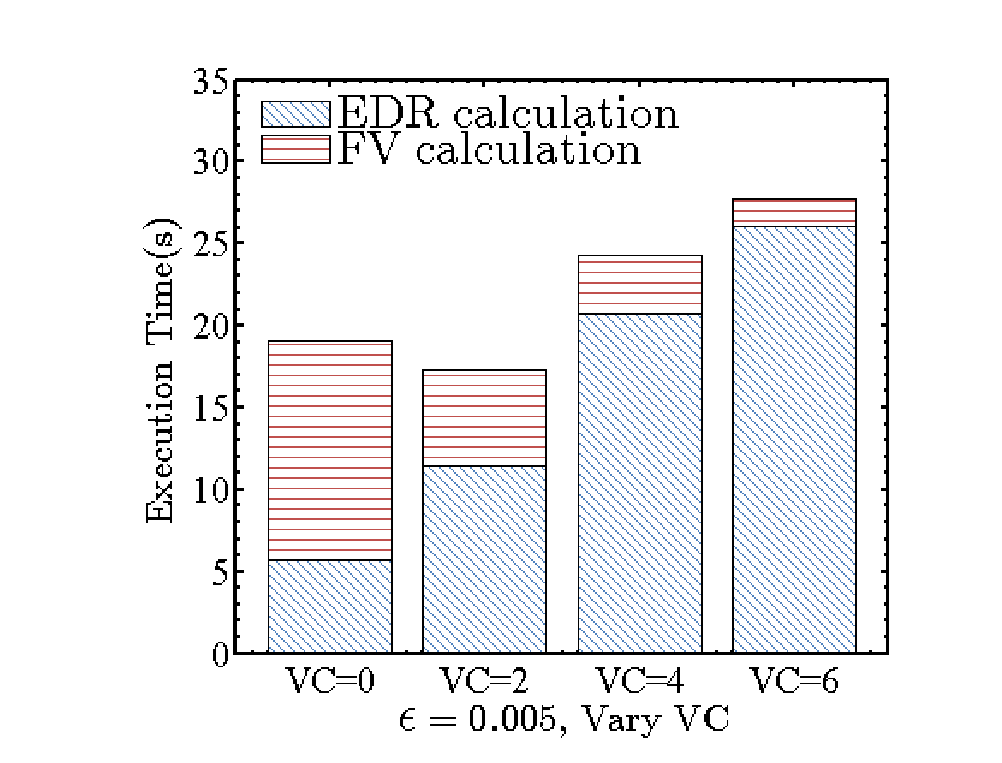
\includegraphics[width=\linewidth]{eps/VC_epsilon.eps}
%			(a) Execution time of 40 top-k similarity queries with different query trajectory length
%		\end{minipage}
%		\hfill
%		\begin{minipage}{0.48\linewidth}
%			\centering
%			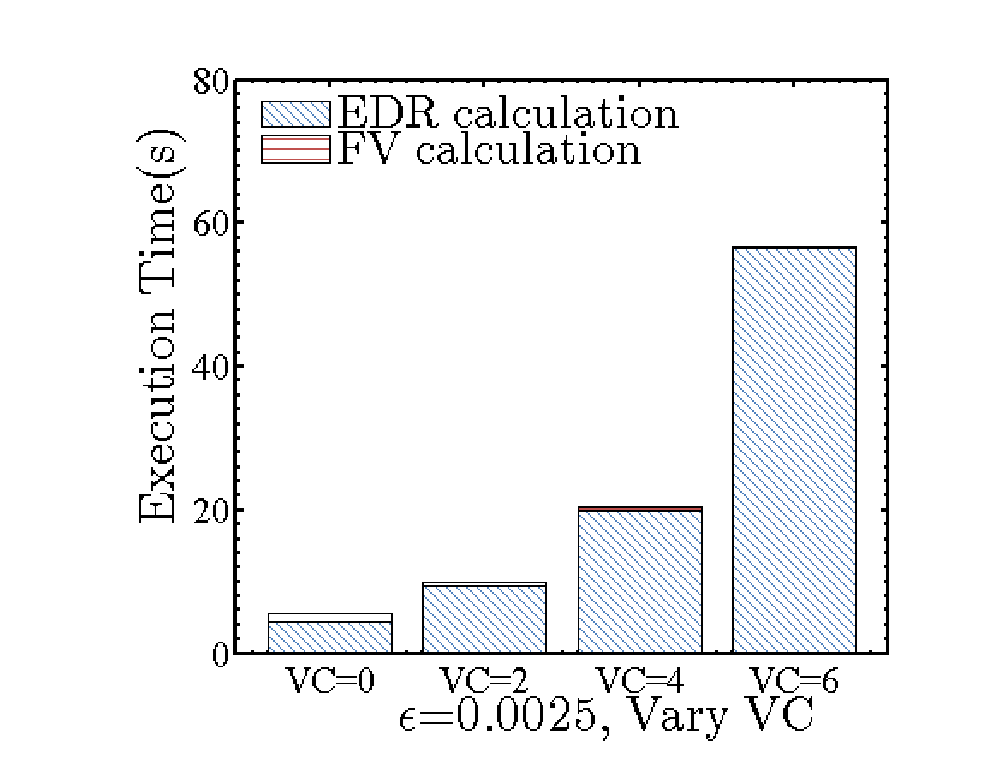
\includegraphics[width=\linewidth]{eps/VC_epsilon_GEO.eps}
%			(b) Speedup ratio of 40 top-k similarity queries with different query trajectory length
%		\end{minipage}
%	}
%	\caption{The execution time (left) and speedup ratio achieved (right) in the top-k similarity queries \label{fig:VC}}
%\end{figure}
%
%$VC$ is a system parameter which has effects on the process of pruning, as we described in section V. Because for different $\epsilon$ the most suitable $VC$ value is not the same, we study the effects of $VC$ based on the situation that $\epsilon$ equals 0.005. Figure x shows the change of pruning time and EDR calculation time under different $VC$. It can be seen that the most appropriate $VC$ is 2. When $CV$ is bigger than 2, the total execution time shows an increasing trend because of too many EDR calculation caused by the more coarse index. On the other hand, there is also high total time consumption if $CV$ is 0, and it is because more time is spent in generating FVs when the index is too fine. We can see it is important to set a correct $CV$ for acheiving a better query performance. 
%\noindent \textbf{Effect of $\epsilon$.}~~Figure~\ref{fig:kValue}



\eat{
	%\section{Experimental Evaluation}\label{sec:exp}
	In this section, we conduct experiments based on two real trajectory datasets to verify the performance of \frname.
	
	\subsection{Experiment Setup}
	
	
	
	\noindent \textbf{Datasets.}~~We use two real life trajectory datasets: SHCAR and GeoLife~\cite{DBLP:conf/www/ZhengZXM09}~\cite{DBLP:conf/huc/ZhengLCXM08}~\cite{DBLP:journals/debu/ZhengXM10}. SHCAR contains the trajectories of 9,446 private cars in Shanghai City collected from 2014 to 2015. GeoLife dataset is published by Microsoft Research Asia, which contains the trajectories from 182 users during Apr. 2007 to Aug. 2012. Most of the sample points of it are within Beijing. Table~\ref{tab:datasets} provides the details of two datasets.
	
	
	
	\noindent \textbf{Data Preprocessing.}~~In our experiment, we split the sequence of sample points from a single user into several subsequences as raw trajectories, in which the timestamp gaps between points are smaller than 30 minutes.  
	%we seem the sequence of sample points of a the same user as a trajectory. If the difference between two time stamps of consecutive points in a trajectory is larger than 30 minutes, we call this point a ``gap''. We then split the trajectory into several new trajectories according to these gaps. 
	%This is because trajectories with these gaps are usually not meaningful single route, which we usually do not concern about. 
	By this preprocessing all raw trajectories are the routes of a single trip.  
	For example, the point sequence of a single car may includes sample points of the trips from home to office and from office to home, and after spliting two trajectories showing two trips respectively can be generated.
	
	\begin{table}[t]
		% increase table row spacing, adjust to taste
		\renewcommand{\arraystretch}{1.1}
		
		% if using array.sty, it might be a good idea to tweak the value of
		% \extrarowheight as needed to properly center the text within the cells
		\caption{datasets}
		\label{tab:datasets}
		\centering
		% Some packages, such as MDW tools, offer better commands for making tables
		% than the plain LaTeX2e tabular which is used here.
		{\small\centering
			\begin{tabular}{|c|c|c|c|c|}
				\hline
				& \# of $T$ & avg. len($T$) & \# of points & default $|\allcell|$\\
				\hline
				SHCAR & 327,474 & 848 & 75,188,293& 262,144\\ 
				\hline
				GeoLife & 30,325 & 926.4 & 19,143,208& 262,144\\
				\hline
				
			\end{tabular}
		}
	\end{table}
	
	\noindent \textbf{Baselines.}~~ For range query, we implement two state-of-the-art approaches supporting range query on GPU: STIG~\cite{7498315} and FSG~\cite{GPUTaxi}. However, these two systems are designed for high-dimensional points rather than trajectories, so we seem range query as extracting $tid$ of points which are within given range $R$. We also implement our approach on multicore CPU as a baseline method. For similarity query, to the best of our knowledge we are the first to utilize GPU to accelerate similarity query based on distance function of EDR. Therefore, we only implement the origin~\cite{DBLP:conf/sigmod/ChenOO05} of our approach on multicore CPU as the baseline. 
	%we only evaluate range query processing on the sample points in trajectories for these two baselines. 
	
	\noindent $\bullet$ \textbf{STIG~\cite{7498315}.} This approach is based on \emph{kd-tree}~\cite{DBLP:journals/cacm/Bentley75}, in which each leaf node corresponds to a data block rather than a point. We choose in-memory CPU-GPU hybrid strategy of it, which means kd-tree is firstly traversed by CPU and some candidate blocks are returned, then each block is refined by GPU in parallel.
	
	\noindent $\bullet$ \textbf{FSG~\cite{GPUTaxi}.} This approach leverage a flat grid-file based indexing to accelerate point-in-polygon queries for analyzing taxi trip data. Similar to our approach, it firstly find cells which overlap query region, then generate candidate \emph{cell-polygon pairs} and send them to GPU. Next each pair is refined by GPU in parallel.
	
	\noindent $\bullet$ \textbf{GAT-MCPU.} The CPU version of \frname. For range query each candidate block is assigned to a thread of CPU to achieve parallelism. All the parameters are set the same as that of \frname. 
	For similarity query we modify original \emph{Histogram Sequential Scan} approach in~\cite{DBLP:conf/sigmod/ChenOO05} to a multithread version by assigning each query task to a thread. 
	%The parameters of this method are set the same as that in our approach.
	
	\noindent \textbf{Measure.}~~We measure the performance of the approaches via the execution time of a fixed number of queries in a batch, representing the throughput of the query processing. For indexing cost, we measure the time used in building index and the increment of memory occupation after building index. We also use speedup ratio compared to the CPU baseline with single thread to measure the acceleration of \frname.
	
	We run all the experiments on a server equipped with two ten-core Xeon E5-2650 v3 processors clocked at 2.3GHz, 64GB of RAM, 4TB of disk storage and an two-chip NVIDIA Tesla K80 GPU, where each of chip has 2,496 CUDA cores and 12GB graphical memory. Our system is implemented by C++ with CUDA 8.0, and operating system is CentOS 7. We conduct our experiment under various parameter settings. Table \ref{table_param} shows the meaning and range of all parameters, while default values are underlined. Unless otherwise specified, we use the default values.
	
	%\noindent \textbf{Parameters.}~~We conduct our experiment under various parameter settings. Table \ref{table_param} shows the range and default value of all parameters. The parameters are divided into two kinds: (1) query parameters, which act as the condition of trajectory query; (2) system parameters, which reflect the configuration of our framework. When testing query parameters 
	
	\begin{table}[!t]
		% increase table row spacing, adjust to taste
		\renewcommand{\arraystretch}{1.1}
	
		% if using array.sty, it might be a good idea to tweak the value of
		% \extrarowheight as needed to properly center the text within the cells
		\caption{Parameters ranges and default values}
		\label{table_param}
		\centering
		% Some packages, such as MDW tools, offer better commands for making tables
		% than the plain LaTeX2e tabular which is used here.
		{\small\centering
		\begin{tabular}{|c|l|l|}
			\hline
			Param. & Description & Range\\
			\hline
			$n$ & \tabincell{l}{max. \# of quadtree levels} & $7$, $8$, $\underline{9}$, $10$ \\
			\hline
			$\theta_p$ & \tabincell{l}{max. candidate block size} & \tabincell{l}{$200$, $2000$, $8000$,\\ $\underline{20000}$, $200000$} \\
			\hline
			$S_{R}$ & query region area ($km^2$) & \tabincell{l}{$0.002$, $\underline{0.004}$, $0.006$,\\ $0.008$} \\
			\hline
			$k$ & \tabincell{l}{value $k$ in $\simq$} & $5$, $10$, $15$, $\underline{20}$, $25$\\
			\hline
			$\zeta$ & \tabincell{l}{avg. query trajectory length} & \tabincell{l}{$200$, $400$, $600$, $\underline{800}$,\\ $1000$} \\
			\hline
			$N_{\rangeq}$ & \tabincell{l}{\# of range queries} & \tabincell{l}{$40$, $60$, $\underline{80}$, $100$, $120$}\\
			\hline
			$N_{\simq}$ & \tabincell{l}{\# of similarity queries}& \tabincell{l}{$20$, $\underline{40}$, $60$, $80$, $100$}\\
			\hline
	
		\end{tabular}
		}
	\end{table}
	
	
	%\subsubsection{Experiment Overview} ???All other parameters are tuned to the optimal case.
	%
	%After that, the scalability is tested. As there is no method to shut some cores in GPU, we can only test the situation with different number of GPUs.
	%
	%In query performance part, same as the most of previous works, we use query latency as our metric. We compare the query time latency of two kinds of queries in different baselines and state-of-the-art systems in a large query set situation. When testing range query, we randomly generate range queries with different areas and positions and reckon the time consumption during finishing all of queries. To reflect the true working environment as much as possible, the chosen positions are restricted to the central district of Shanghai ($31.11^{\circ} N-31.36^{\circ} N, 121.39^{\circ} E-121.58^{\circ} E$). For similarity query, some trajectories are selected randomly from dataset as the query set. During the query, for each trajectory in query set, the result of top-$k$ similarity query is returned under the settings of different query parameters including $k$ and $\epsilon$. Queries are handled with formed query set and time consumption in both baseline method and GTS are then calculated. 
	
	
	
	\subsection{Comparison of Various Approaches}
	
	In this section we compare the throughput of our approach with the baseline methods.
	% mentioned before in range query and top-$k$ similarity query. 
	%Execution time under different number of queries in a batch on two datasets is measured as the metric of throughput.
	
	\begin{figure}[!t]
		\centering
	\scriptsize{
		\begin{minipage}{0.48\linewidth}
			\centering
			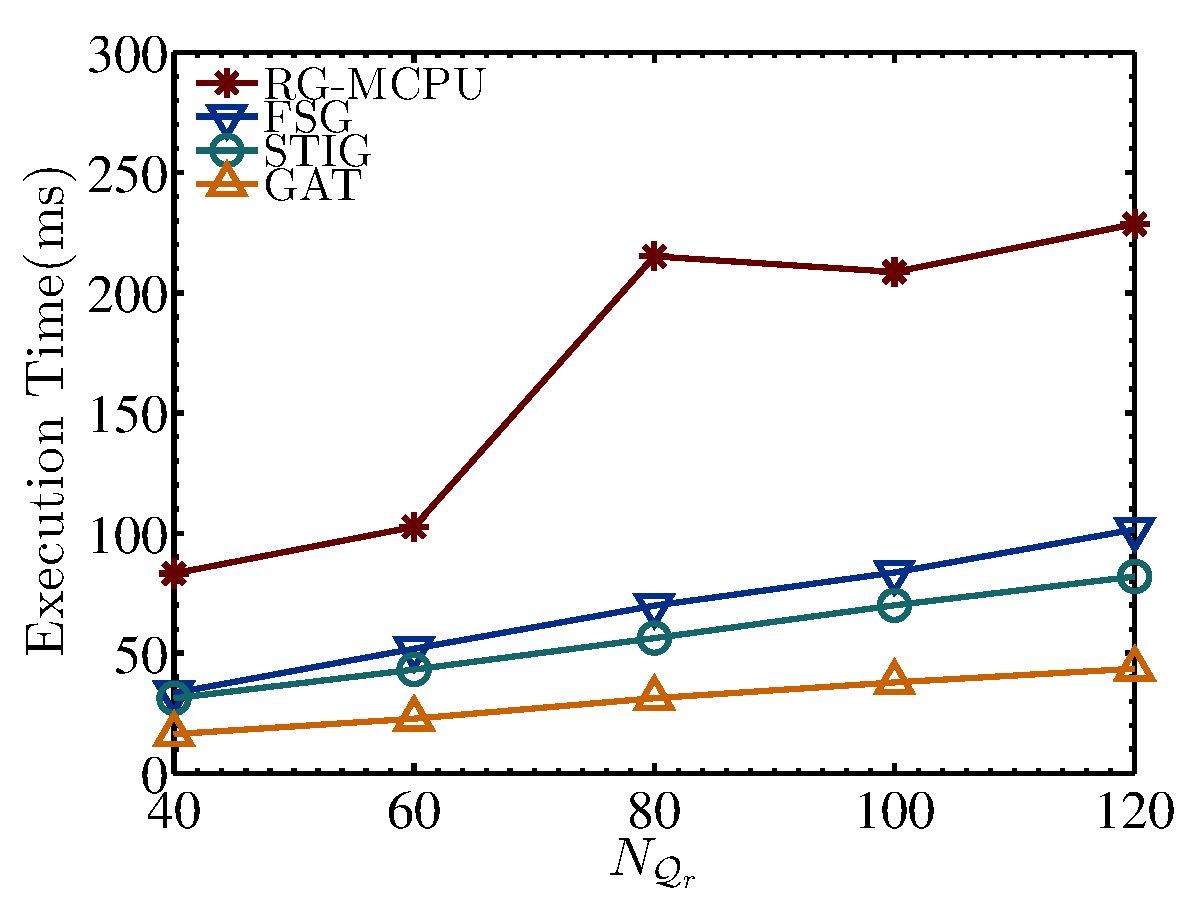
\includegraphics[width=\linewidth]{eps/QueryNum_RangeQ.eps}
			(a) Range Query
		\end{minipage}
		\hfill
		\begin{minipage}{0.48\linewidth}
			\centering
			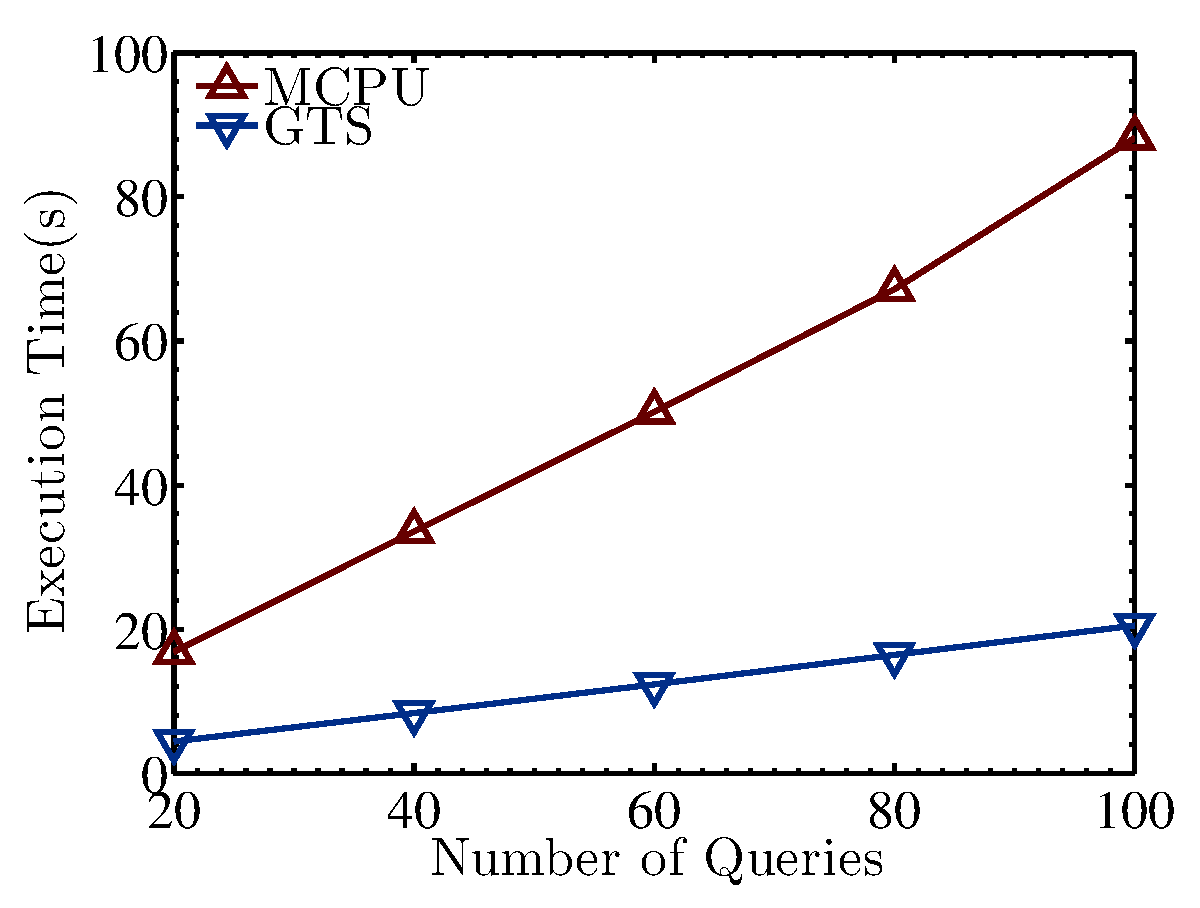
\includegraphics[width=\linewidth]{eps/QueryNum_SimilarityQ.eps}
			(b) Similarity Query
		\end{minipage}
	}
		\caption{Throughput under different workload on SHCAR\label{fig:QueryNum}}
	\end{figure}
	
	\begin{figure}[!t]\centering
		\scriptsize{
			\begin{minipage}{0.48\linewidth}
				\centering
				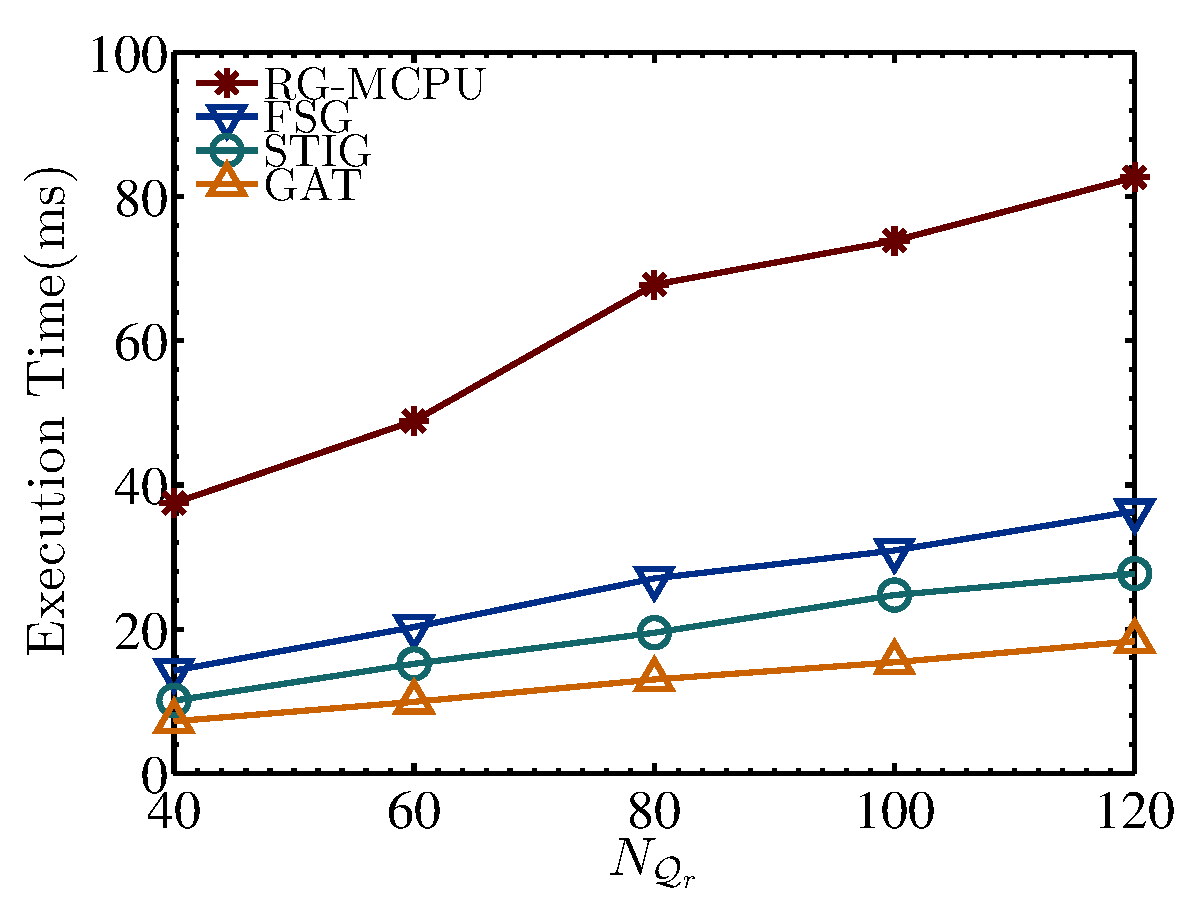
\includegraphics[width=\linewidth]{eps/QueryNum_RangeQ_GEO.eps}
				(a) Range Query
			\end{minipage}
			\hfill
			\begin{minipage}{0.48\linewidth}
				\centering
				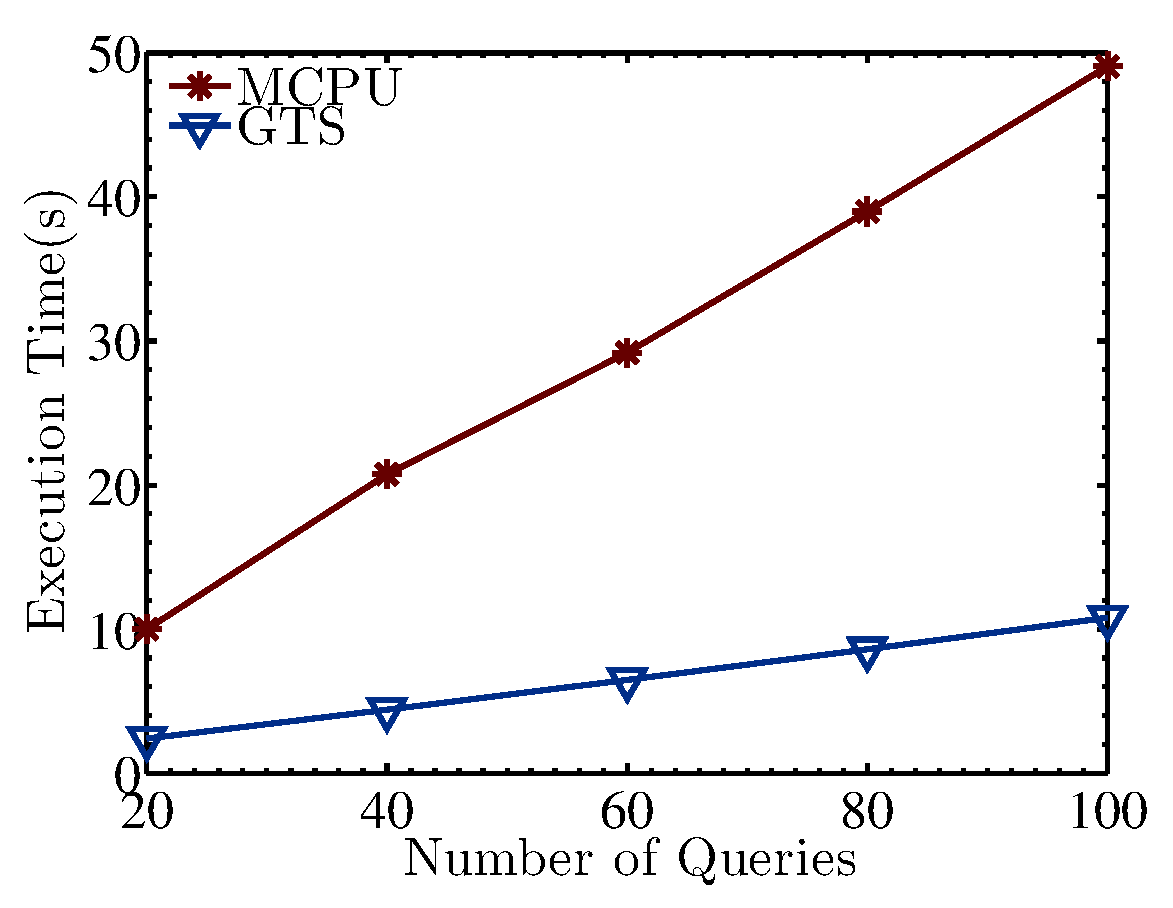
\includegraphics[width=\linewidth]{eps/QueryNum_SimilarityQ_GEO.eps}
				(b) Similarity Query
			\end{minipage}
		}
		\caption{Throughput under different workload on GeoLife\label{fig:QueryNum_GEO}}
	\end{figure}
	
	\noindent \textbf{Range Query.}~~Figure~\ref{fig:QueryNum}(a) and figure~\ref{fig:QueryNum_GEO}(a) shows the execution time with different number of range queries on SHCAR and Geolife. Overall, the execution time in four approaches increases as the rising scale of queries.
	we can see that our approach outperforms other three baselines, and the execution time increases linearly with the number of queries in a batch. 
	FSG and STIG perform worse than \frname, because of too much cost in data transfering between GPU and main memory. In \frname, this cost is reduced owing to the memory allocation table. 
	We can also see that STIG works better than FSG, because in STIG a \emph{kd-tree} like index guarantees the even division of blocks, leading to more balanced load. This benefit is also achieved by \frname.
	%In \frname hundreds of queries can be finished within $50$ ms, which meet the requirement of real-time service.
	
	\noindent \textbf{Similarity Query.}~~Figure~\ref{fig:QueryNum}(b) and figure~\ref{fig:QueryNum_GEO}(b) shows the execution time with different number of top-$k$ similarity queries. Two methods both show a linear increment in time consumption with the scale of queries. 
	We can see that \frname approach we proposed outperforms EDR-MCPU under all $N_\rangeq$
	%, and as the increasing number of queries, the gap of the performance between these two methods becomes larger.
	The result shows that the GPU-based acceleration of EDR calculation, which is the main source of the computational cost in top-$k$ similarity query, improves the throughput significantly. 
	
	%\begin{figure}[!t]\centering
	%	\includegraphics[width=8cm]{pdf/SpeedUp.pdf}
	%	\caption{Speedup ratio of both range query and top-k similarity query on one GPU and two GPUs respectively, compared to the single-core CPU implementation\label{fig:SpeedUp}}
	%\end{figure}
	
	
	
	
	
	\subsection{Indexing Cost}
	
	\begin{figure}[!t]\centering
		\scriptsize{
			\begin{minipage}{0.48\linewidth}
				\centering
				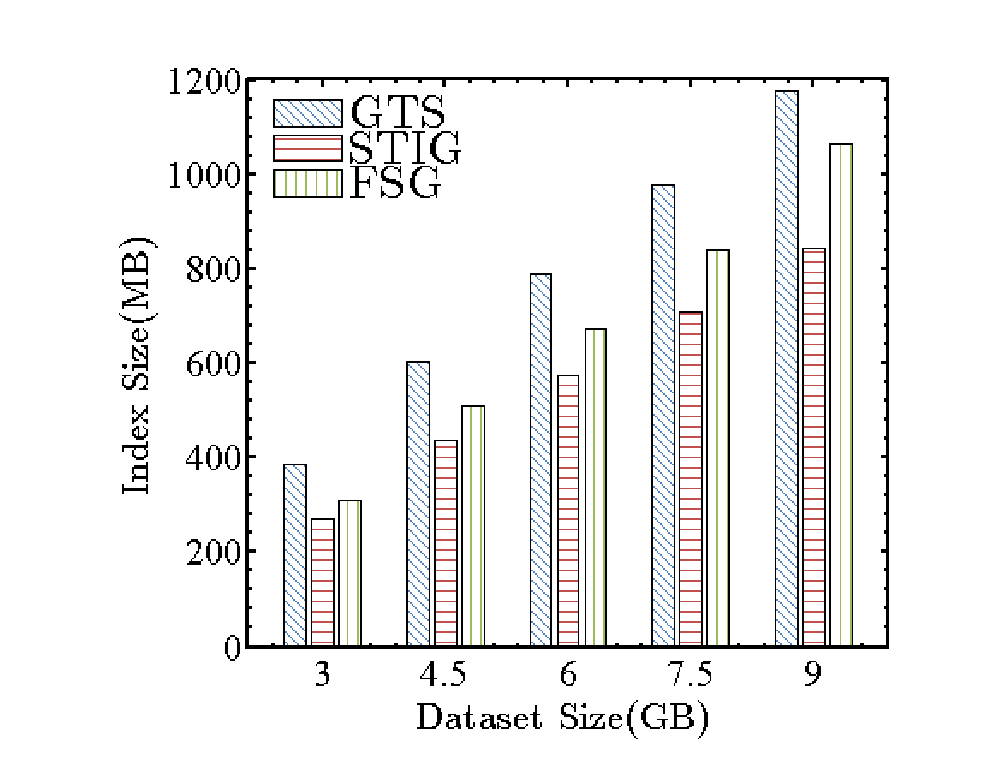
\includegraphics[width=\linewidth]{eps/indexSize.eps}
				(a) Memory Occupation
			\end{minipage}
			\hfill
			\begin{minipage}{0.48\linewidth}
				\centering
				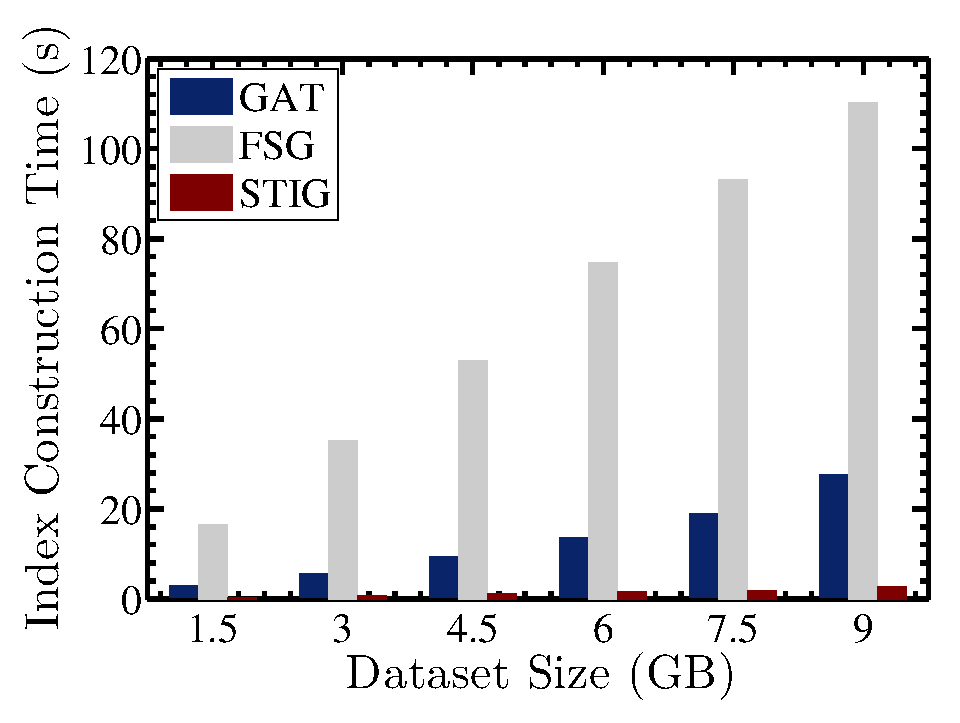
\includegraphics[width=\linewidth]{eps/indexTime.eps}
				(b) Indexing Construction Time
			\end{minipage}
		}
		\caption{Indexing Cost\label{fig:IndexCost}}
	\end{figure}
	
	We test the indexing cost including memory cost and index construction time for all GPU-based baselines. The result is shown in figure \ref{fig:IndexCost}. All the parameters are set to default. 
	
	\noindent \textbf{Memory Cost.}~~From figure~\ref{fig:IndexCost}(a), it can be seen that the memory cost increases as the growth in the scale of dataset.
	There is a small increment of memory cost in \frname compared to two other GPU-based methods. The main reason is because the extra trajectory index which makes \frname able to support trajectory representation and sufficient histogram-based pruning in similarity queries is not maintained in STIG and FSG.
	In the evaluation of $9$GB dataset only about $80$MB to $290$MB more memory is consumed compared to FSG ($1063$MB) and STIG ($853$MB), it is an acceptable cost considering the big increment on throughput in \frname.
	
	\noindent \textbf{Index Construction Time.}~~From figure \ref{fig:IndexCost}(b), we can see the indexing time grows with larger dataset. \frname spends less time in building index than STIG, because in STIG there is a large amount of computation of finding medium values when generating kd-tree. 
	There is an additional quadtree-like index in \frname, so more construction time is used compared to FSG.
	
	\subsection{Speedup}
	In this section we study the speedup attained by our \frname framework under default parameters with one and two GPUs. For comparison a single thread is created to execute the queries in implementation on CPU. This study explains two benefits. First, it shows that our GPU-based implementation can outperform traditional implementation on CPU. Second, it demonstrates that a near-linear improvement of efficiency can be achieved by adding more GPU devices.
	
	\begin{table}[t]
		\centering
		
		\caption{Speedup achieved in two datasets}     % NOTE!  caption goes _before_ the table contents !!
		\label{tab:speedup}
		
		\begin{small}
			\begin{tabular}{|l|c|c|c|c|}
				\hline
				{\bfseries Dataset} & \multicolumn{2} {c|} {\bfseries SHCAR} & \multicolumn{2} {c|} {\bfseries GeoLife} \\
				\cline{1-5}
				{\bfseries \# GPU} & {\bfseries 1GPU} &  {\bfseries 2GPU}  & {\bfseries 1GPU} &  {\bfseries 2GPU}  \\
				\hline
				Range Query & 20.07 & 37.63 & 18.03 & 32.43 \\
				\hline
				Top-k Similarity Query & 35.54 & 68.53 & 38.94 & 74.95 \\
				\hline
			\end{tabular}
		\end{small} 
	\end{table}
	
	Table \ref{tab:speedup} shows the speedup ratio for two kinds of queries. 
	Our approach achieves up to 38.94x speedup in evaluation of top-$k$ similarity query for single GPU, and 74.95x in dual GPUs environment. The high speedup ratio comes from the parallel execution of compute-intensive EDR calculation. 
	For range query, a lower speedup ratio of 20.07x for single GPU and 37.63x for dual GPUs is achieved. Considering that only some comparison operations need to be performed in varification procedure, the larger propotion of data transfering cost restricts the speedup ratio compared to similarity query.
	
	\subsection{Scalability}
	
	We investigate the scalability of all of the approaches in this part. Figure~\ref{fig:Scalability} presents the results under different size of data in the range from $3$GB to $9$GB.
	
	\begin{figure}[!t]\centering
			\scriptsize{
			\begin{minipage}{0.48\linewidth}
				\centering
				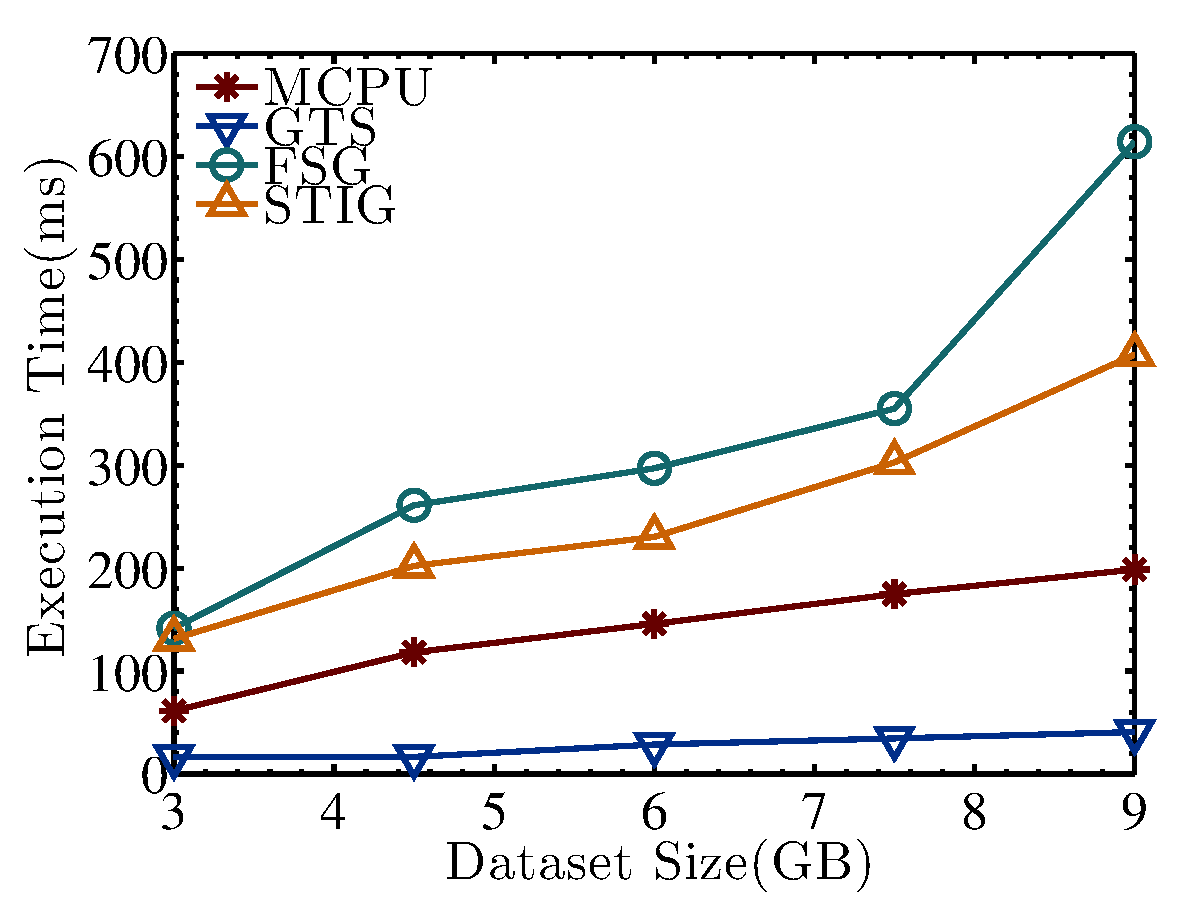
\includegraphics[width=\linewidth]{eps/range_scala.eps}
				(a) Range Query
			\end{minipage}
			\hfill
			\begin{minipage}{0.48\linewidth}
				\centering
				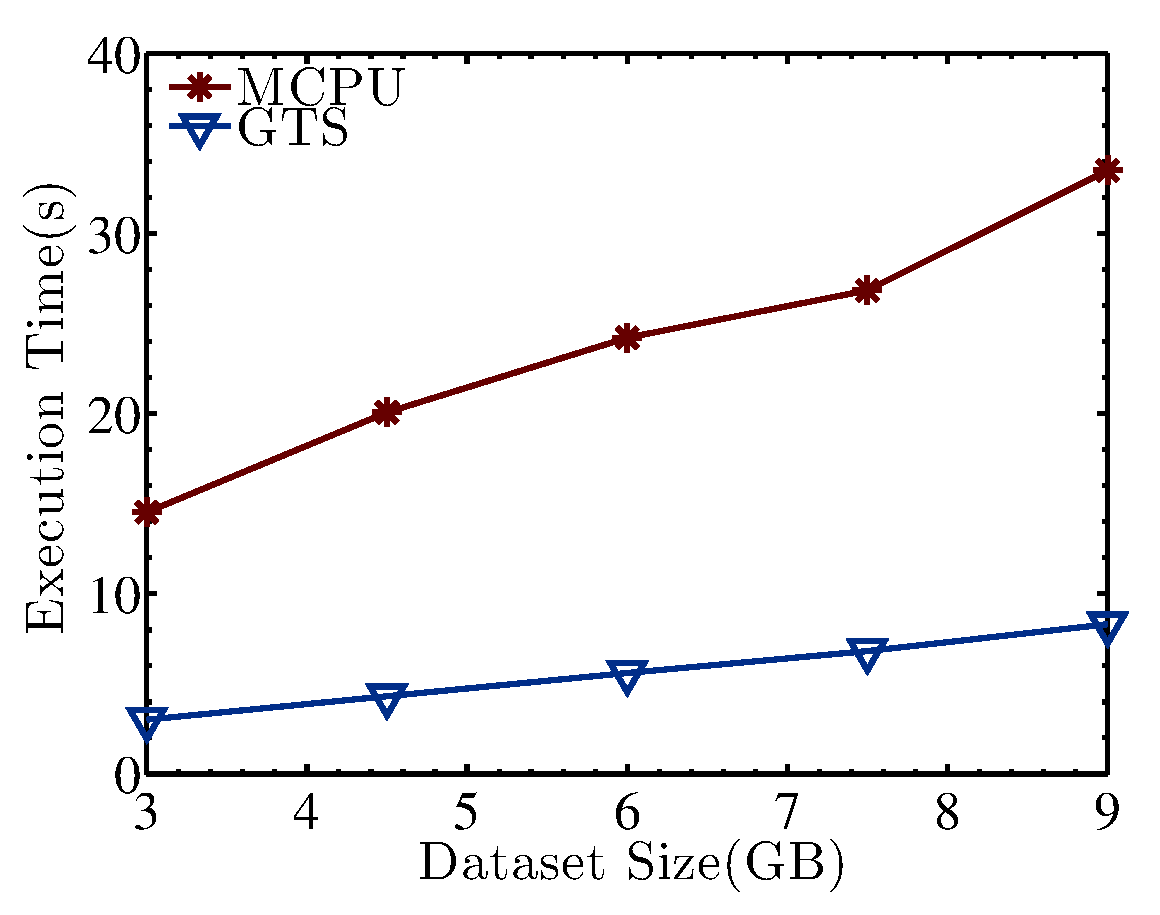
\includegraphics[width=\linewidth]{eps/similarity_scala.eps}
				(b) Similarity Query
			\end{minipage}
		}
		\caption{Scalability\label{fig:Scalability}}
	\end{figure}
	
	\noindent \textbf{Range Query.}~~Figure~\ref{fig:Scalability}(a) shows the execution time of a batch of 80 range queries under our \frname framework and three baseline approaches. We can see it is a general trend that execution time increases as larger dataset. This is determined by the fact that more candidates are included in range queries if there are more points in dataset.
	%However, as the growing scale of dataset, the execution time on GPU-based methods show a sub-linear increasing trend. This is because the increment of more expensive data transferring between main memory and GPU is quicker than that of quantity of candidates waiting for verification.\textbf{Why?????????}
	We can also see our approach performs better when facing large scale dataset than other GPU-based baselines, indicating that our system has a good scalability on range query. 
	
	\noindent \textbf{Similarity Query.}~~The execution time of top-$k$ similarity queries on different size of dataset is shown in figure \ref{fig:Scalability}(b). We can see as the growing volume of data, both two approaches consume more time on queries and the benefit of acceleration by using GPU becomes more obvious. It also proves that our system works excellently on large-scale dataset.
	
	
	\subsection{Parameter Tuning}
	
	In this section we study the effects of parameters in \frname. Here are totally five parameters other than $N_\rangeq$ and $N_\simq$ in our experiment as Table~\ref{table_param} shows. 
	%Some of them can be categorized as query parameters, which are properties of queries and can be evaluated in both other systems and GTS, such as the area of MBR and $k$. Others are system parameters, which only exist in our system. For this reason, we show results of all baselines when evaluating the execution time in different query conditions to demonstrate both the expected performance in various environment and the effects of these parameters. Meanwhile, system parameters are evaluated under different query scales to show the effects, which are only based on our approach. 
	
	%\noindent \textbf{Range Query.}~~There are three parameters about range query: $S_R$, $\theta_p$ and $n$. We will evaluate the effects of them.
	
	\begin{figure}[!t]\centering
		\scriptsize{
			\begin{minipage}{0.48\linewidth}
				\centering
				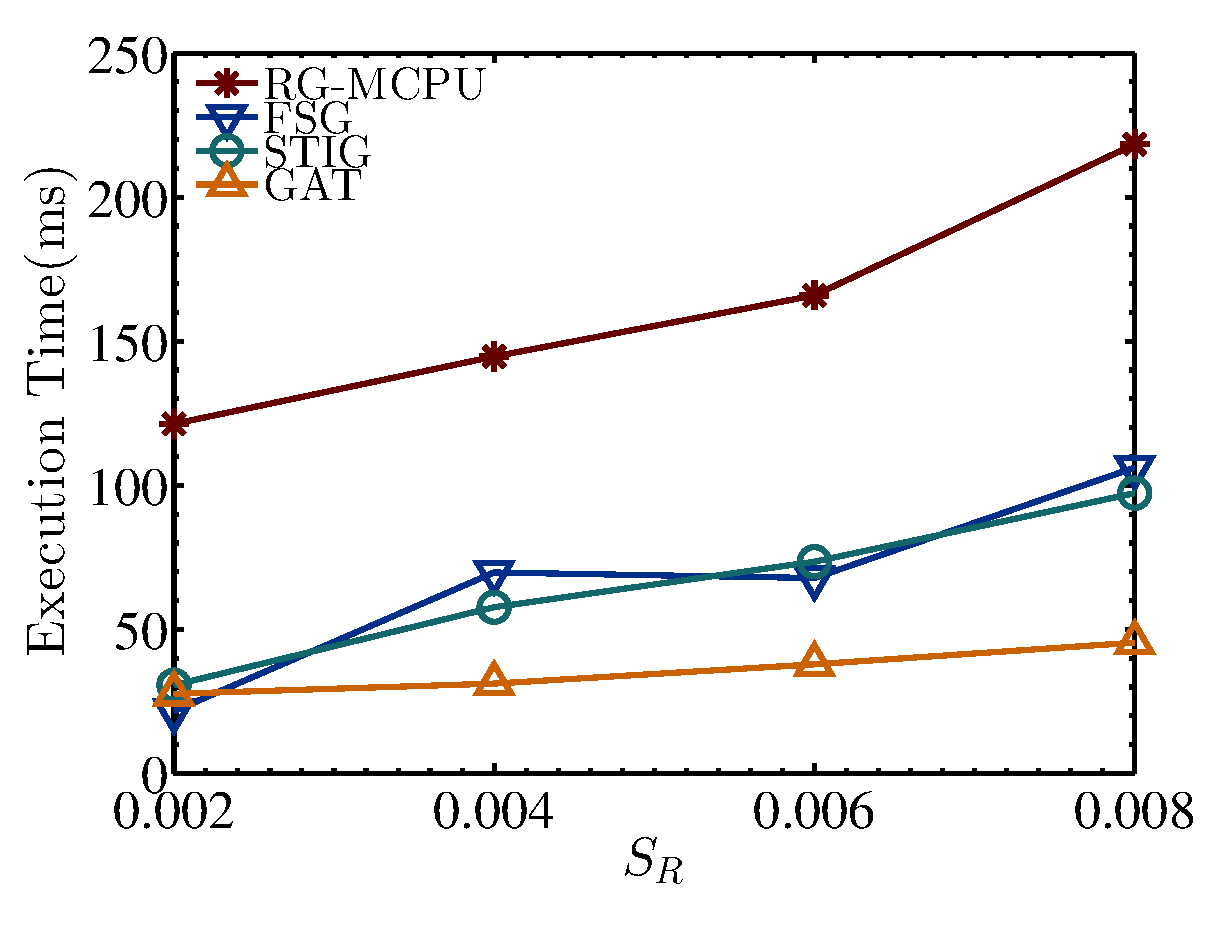
\includegraphics[width=\linewidth]{eps/RangeArea.eps}
				(a) SHCAR
			\end{minipage}
			\hfill
			\begin{minipage}{0.48\linewidth}
				\centering
				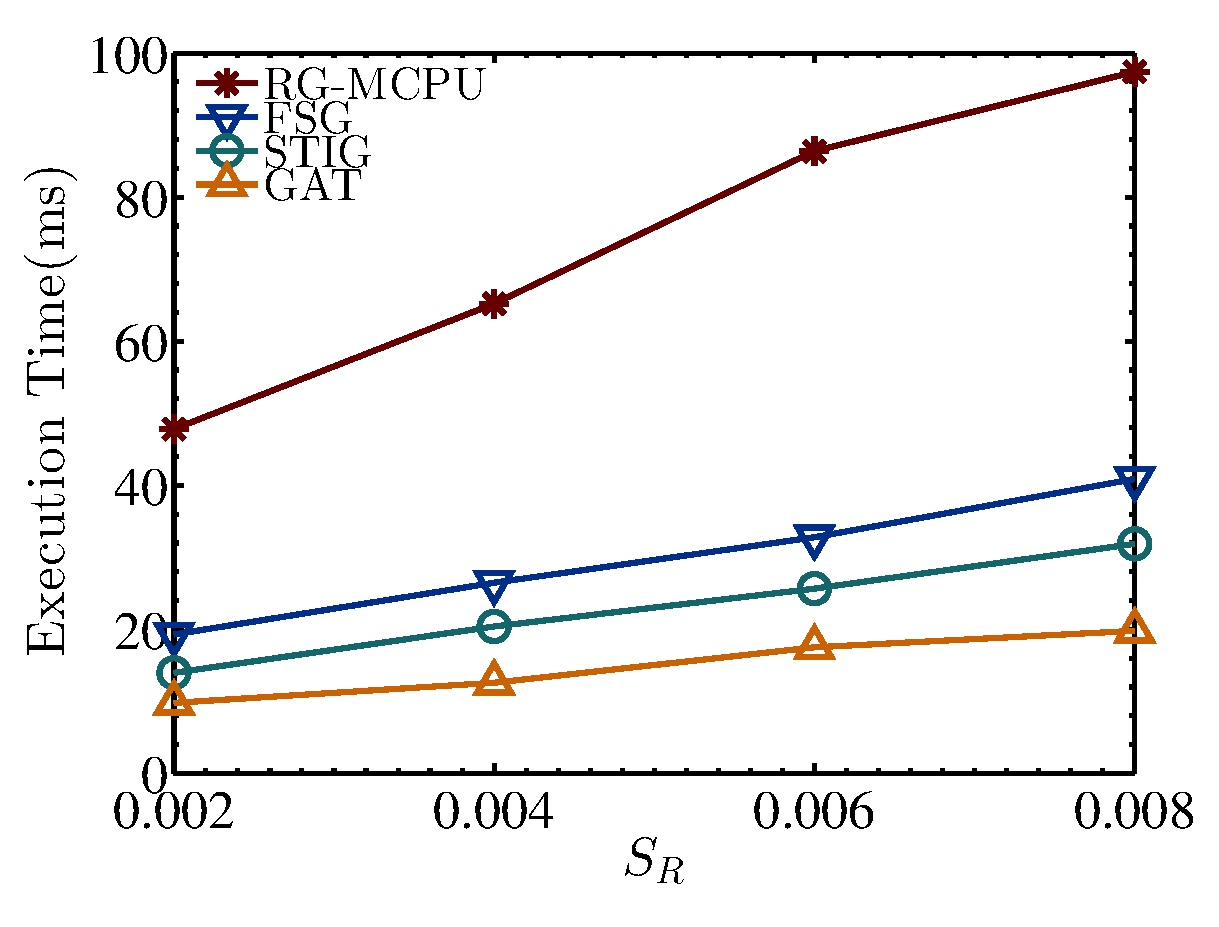
\includegraphics[width=\linewidth]{eps/RangeArea_GEO.eps}
				(b) GeoLife
			\end{minipage}
		}
		\caption{Effects of area of query region ($R_{\rangeq}$) \label{fig:RANGE}}
	\end{figure}
	
	% zbw: in this part the unit of area can be transfromed into standard unit
	\noindent \textbf{Effect of query region area $S_R$.}~~$S_{R}$ indicates the area of query region, which directly controls the selectivity of range query. Figure~\ref{fig:RANGE} shows the execution time of queries with different $S_{R}$, which are generated by extending from a same coordinate in the city center.
	We can see in all approaches, the time consumption rises as the area of $R$ increases from $0.002$ to $0.008$, because more candidate blocks overlap with $R$ waiting for verification as the growing query region. We can see that this trend is nearly linear for our framework, because the scale of verification and the number of nodes overlapped by query region $R$ are basically propotional to the area of it. 
	Our frameworks shows a better throughput even in the query region with a large area. 
	
	
	\begin{figure}[!t]\centering
		\scriptsize{
			\begin{minipage}{0.48\linewidth}
				\centering
				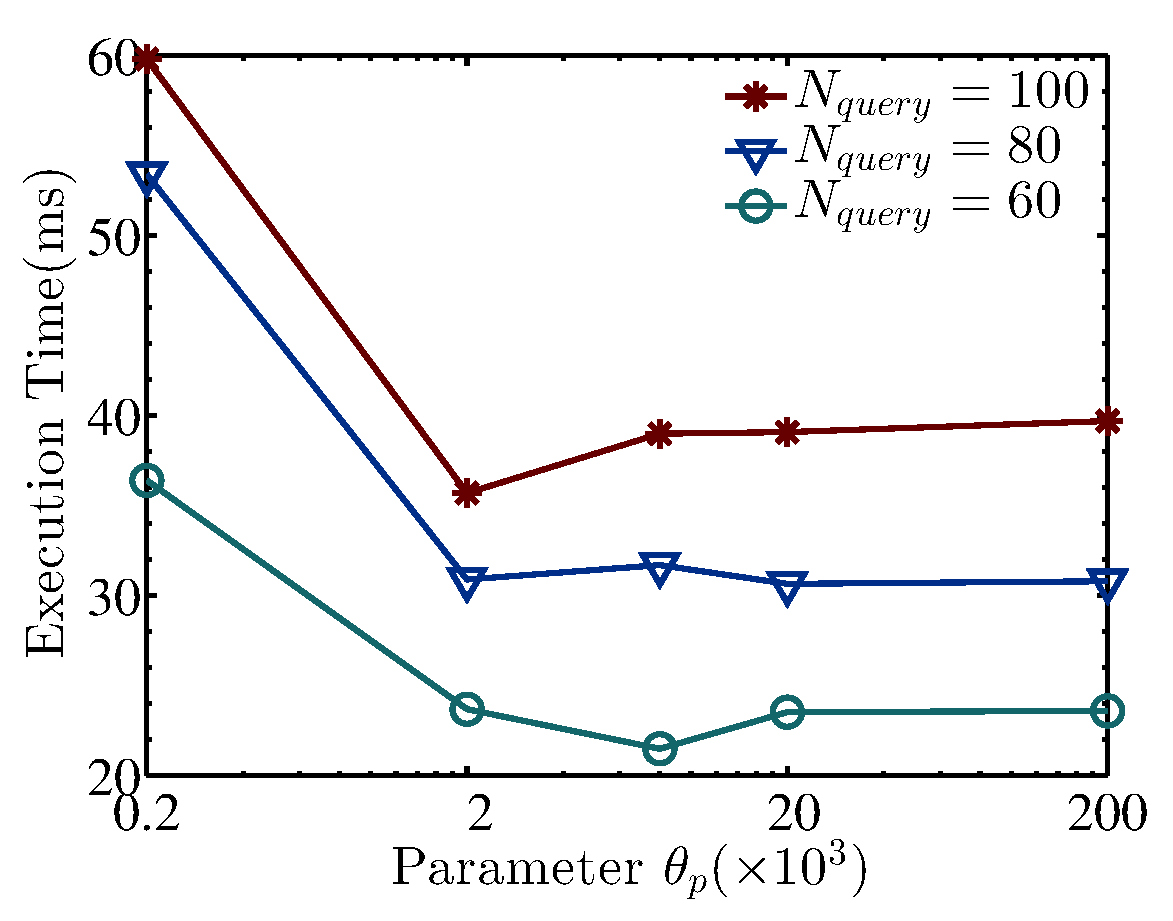
\includegraphics[width=\linewidth]{eps/MCELL.eps}
				(a) SHCAR
			\end{minipage}
			\hfill
			\begin{minipage}{0.48\linewidth}
				\centering
				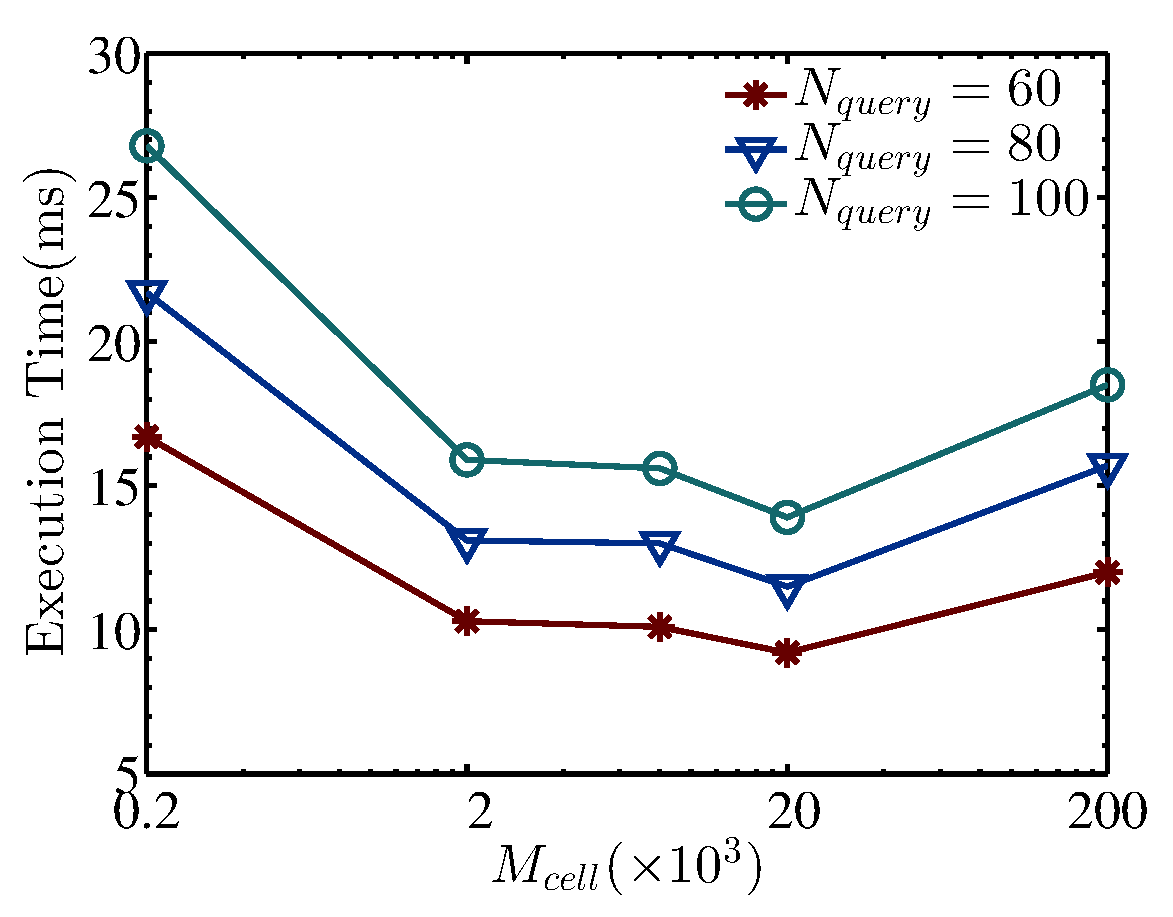
\includegraphics[width=\linewidth]{eps/MCELL_GEO.eps}
				(b) GeoLife
			\end{minipage}
		}
		\caption{Effects of maximal \#points covered by a leaf node ($\theta_p$) \label{fig:MCELL}}
	\end{figure}
	\noindent \textbf{Effect of maximal candidate block size $\theta_p$.}~~Figure \ref{fig:MCELL} shows the results of our approach in range query when we vary the parameter $\theta_p$, under there different workloads.
	%of $N_{\rangeq}=60$, $N_{\rangeq}=80$ and $N_{\rangeq}=100$. 
	We can see under about $\theta_p=8000$ and $\theta_p=20000$ our approach achieves the best performance on both datasets respectively. 
	There is a downward trend of execution time as decreasing $\theta_p$, because if $\theta_p$ is too small, each SM of GPU need only finish several comparison operations between points and the query region (e.g., less than the number of cores in SM), leading to not fully usage of GPU. 
	On the other hand, in the result of Geolife, as $\theta_p$ continues to increase from $20000$, the execution time goes up slightly. This is because the workload of verification tasks on each SM becomes extremely large, so the absolute gap among the cost of each task is indeed bigger, leading to an unbalanced workload.
	
	\begin{figure}[!t]\centering
		\scriptsize{
			\begin{minipage}{0.48\linewidth}
				\centering
				\includegraphics[width=\linewidth]{eps/n_FD.eps}
				(a) SHCAR
			\end{minipage}
			\hfill
			\begin{minipage}{0.48\linewidth}
				\centering
				\includegraphics[width=\linewidth]{eps/n_filter.eps}
				(b) GeoLife
			\end{minipage}
		}
		\caption{Effects of maximal \#level of $\treeindex $ ($n$) \label{fig:LCELL}}
	\end{figure}
	\noindent \textbf{Effect of maximal number of quadtree level $n$.}~~Parameter $n$ controls the number of cells in $\allcell$. 
	Figure \ref{fig:LCELL} shows the result when parameter $n$ varying from $7$ to $10$.
	%We can see the there is only slight change of performance. This is because the cells are grouped into blocks during filtering phase as the unit of task assignment, so the change of the number and size of cells do not affect the task division and varification scale in each SM significantly, which are the main factors of the performance.
	We can see as the growth of $n$, the time consumption of calculating frequency distance increases, while that of the iteration between generating candidates and calculating EDR decreases. The reason of this change is that the length of frequency vectors are exponential to the parameter $n$, which is propotion to the computational cost of frequency distance.
	
	%\noindent \textbf{Similarity Query.}~~In this section, we study the effects of parameters in top-$k$ similarity query, including $k$ and $\zeta$.
	
	
	\begin{figure}[!t]\centering
		\scriptsize{
			\begin{minipage}{0.48\linewidth}
				\centering
				\includegraphics[width=\linewidth]{eps/kValue.eps}
				(a) SHCAR
			\end{minipage}
			\hfill
			\begin{minipage}{0.48\linewidth}
				\centering
				\includegraphics[width=\linewidth]{eps/kValue_GEO.eps}
				(b) GeoLife
			\end{minipage}
		}
		\caption{Effects of $k$ \label{fig:kValue}}
	\end{figure}
	
	\noindent \textbf{Effect of $k$.}~~Figure~\ref{fig:kValue} shows the execution time of top-$k$ similarity query under different value of $k$. We can see that for all $k$ values our approach achieves better performance than CPU-based implementation.
	In both two approaches, execution time goes higher as the $k$ value increases. This is because under a larger $k$ more EDR should be calculated before reaching terminate condition. The amplitude of increment in the number of EDR calculation becomes smaller as $k$ grows, so the execution time tends to be constant after $k$ is large enough. 
	
	
	
	\begin{figure}[!t]\centering
				\scriptsize{
			\begin{minipage}{0.48\linewidth}
				\centering
				\includegraphics[width=\linewidth]{eps/QueryLength.eps}
				(a) Execution time
			\end{minipage}
			\hfill
			\begin{minipage}{0.48\linewidth}
				\centering
				\includegraphics[width=\linewidth]{eps/trajLength_GEO.eps}
				(b) Speedup ratio
			\end{minipage}
		}
		\caption{Effects of query trajectory length ($\zeta$) \label{fig:LENSIMI}}
	\end{figure}
	
	\noindent \textbf{Effect of average query trajectory length $\zeta$.}~~We then study the effects of $\zeta$ in top-$k$ similarity query. In each test, we choose ten different trajectories of the same length as query trajectories and reckon the execution time.
	%To concern on the effects of trajectories' length, We control the factor of different FD calculation cost in by using trajectories with the same cell-based trajectory but different length to form a query set.
	Figure \ref{fig:LENSIMI} shows the execution time and speedup ratio under different length of query trajectory. It can be seen that speedup ratio rises linearly as the growing length of query trajectory, meaning that our approach can achieve a higher speedup for longer query trajectory. The reason of this phenomenon is that the cost of each EDR calculation is mainly determined by number of iteration, which is linear with the length of query trajectory.
	
	%\noindent \textbf{Effect of $n$.}~~
	%\begin{figure}[!t]\centering
	%	\scriptsize{
	%		\begin{minipage}{0.48\linewidth}
	%			\centering
	%			\includegraphics[width=\linewidth]{eps/VC_epsilon.eps}
	%			(a) Execution time of 40 top-k similarity queries with different query trajectory length
	%		\end{minipage}
	%		\hfill
	%		\begin{minipage}{0.48\linewidth}
	%			\centering
	%			\includegraphics[width=\linewidth]{eps/VC_epsilon_GEO.eps}
	%			(b) Speedup ratio of 40 top-k similarity queries with different query trajectory length
	%		\end{minipage}
	%	}
	%	\caption{The execution time (left) and speedup ratio achieved (right) in the top-k similarity queries \label{fig:VC}}
	%\end{figure}
	%
	%$VC$ is a system parameter which has effects on the process of pruning, as we described in section V. Because for different $\epsilon$ the most suitable $VC$ value is not the same, we study the effects of $VC$ based on the situation that $\epsilon$ equals 0.005. Figure x shows the change of pruning time and EDR calculation time under different $VC$. It can be seen that the most appropriate $VC$ is 2. When $CV$ is bigger than 2, the total execution time shows an increasing trend because of too many EDR calculation caused by the more coarse index. On the other hand, there is also high total time consumption if $CV$ is 0, and it is because more time is spent in generating FVs when the index is too fine. We can see it is important to set a correct $CV$ for acheiving a better query performance. 
	%\noindent \textbf{Effect of $\epsilon$.}~~Figure~\ref{fig:kValue}
}

\section{Related Work}\label{sec:related}

In this sectoin we review some previous related works about Trajectory Indexing and GPU-accelerated Spatial Query Processing.

\subsection{Trajectory Indexing}

R-Tree~\cite{DBLP:conf/sigmod/Guttman84} is the most classical index for spatial data, which is the two-dimensional generalization of B-Tree~\cite{DBLP:conf/sigmod/BayerM70}.
After that some indices optimized for trajectory such as 3D-RTree~\cite{DBLP:conf/icmcs/TheodoridisVS96}, TB-Tree~\cite{DBLP:conf/vldb/PfoserJT00} and TPR-Tree~\cite{DBLP:conf/sigmod/SaltenisJLL00}. They index on the temporal dimension as well as the spatial dimension.
% However, they are non-adaptive, meaning that they suffered from a performance loss as the diversity of trajectory distribution. 
SETI~\cite{DBLP:conf/cidr/ChakkaEP03} proposed a indexing mechanism which forms a two-level index by decoupling the spatial dimension and temporal dimension to reduce the complexity of spatial query. 
PIST~\cite{DBLP:journals/geoinformatica/BoteaMNS08} developed a cost model of partitioning the data space for different data distributions, aiming to reduce the number of disk accesses. 
TrajStore~\cite{DBLP:conf/icde/Cudre-MaurouxWM10} proposed an adaptive algorithm to split trajectories optimally and cluster them physically to achieve a lowest expected I/O cost.
Wang et.al. developed an in-memory column-oriented storage called SharkDB~\cite{DBLP:conf/cikm/WangZXZZS14} to achieve the high performance in range queries and kNN queries and avoid the expensive I/O operations. 
Trajtree~\cite{EDWP15} was designed to index the computation of EDwP, a similarity metric optimized for trajectories under inconsistent sampling rates. 
However, these works are all designed to process queries on CPU, so throughput in them under big trajectory dataset is limited comparing to our \frname framework.

\subsection{GPU-accelerated Spatial Query Processing}
GPU has been used for accelerating the query processing for both spatial-temporal data including trajectory. Zhang et.al~\cite{Zhang:2012:USH} proposed a prototype system called U$_2$STRA to manage large-scale trajectory data efficiently using GPU. It proposed a four-level hierarchy to split and represent trajectories, and then index them by a grid-file based data structure. Based on this system, a top-$k$ similarity query algorithm called TKSimGPU~\cite{DBLP:conf/bigdataconf/LealGZY15} is developed. It calculate Hausdorff distance between two trajectories by distributing the tasks of computing  the distance of subsequences in different cells to GPU cores and then merge the results. However, TKSimGPU failed in the supporting of some popular and robust distance functions such as EDR~\cite{DBLP:conf/sigmod/ChenOO05}, DTW~\cite{DBLP:conf/vldb/Keogh02} and EDwP~\cite{EDWP15}, because the task division strategy of it only support considering matching points within one cell in a subtask.
%However, Hausdorff is not as popular and robust as the distance functions based on global alignment such as EDR~\cite{DBLP:conf/sigmod/ChenOO05}, DTW~\cite{DBLP:conf/vldb/Keogh02} and EDwP~\cite{EDWP15}, requiring all the matching cases of any two points in whole trajectories are considered during the computation. Therefore the task division strategy of TKSimGPU failed in these distance funcitons because only points within the cell can be used in a subtask.
For another thing, the grid-file based data structure will suffer from unbalanced load when the distribution of dataset is not uniform, because the quantities of points in different cells differ dramatically.

Lettich et.al~\cite{DBLP:conf/gis/LettichOS15} designed the PR-quadtree to process stream spatial k-NN queries. Similar to our work, it builds a quadtree as the index to achieve load balancing in query processing. But different from our \frname framework, both index construction and query processing are finished in GPU in this work, because the scale of stream spatial data is usually not so large and they can be fully loaded into global memory.  
Zhang et.al~\cite{GPUTaxi} developed a query processing system with a a grid-file based data structure to manage big taxi trip data. 
Doraiswamy et.al.~\cite{7498315} generalized the kd-tree to STIG, in which points in leaf node are packed to a block to guarantee the fully utilization of GPU when performing interative spatio-temporal queries on it. 
However, it is not suitable for managing large-scale trajectory data, because trajectory contains not only spatio-temporal informations, but also the connective information among the points in a sequence.  

%Some works utilize distributed system to solve the efficiency problem in processing spatial queries on single CPU. 
%HadoopGIS ~\cite{DBLP:journals/pvldb/AjiWVLL0S13} adapted and extended Hadoop to meet the challenge of large-scale spatial objects and high computation complexity. It is intergrated with Hive and provides an expressive spatial query language. 
%Lu et.al~\cite{DBLP:journals/pvldb/LuSCO12} proposed a solution to the problem of implementing kNN join, an expensive spatial operation for large dataset, in MapReduce to improve the performance of it. Aiming to the performance degradation due to the moving hotspots in distributed spatio-temporal storage system, 
%Pyro~\cite{DBLP:conf/usenix/LiHGSA15} adapted HDFS and H-Base by employing a novel DFS block grouping algorithm and multi-scan optimization to reduce the response time of geometry queries. 
%Based on Spark, Dong et.al developed Simba ~\cite{DBLP:conf/sigmod/XieL0LZG16} to provide native support for spatial queries to achieve low query latency and high throughput and excellent scalability. 
%After that, he proposed a distributed framework~\cite{DBLP:journals/pvldb/XieLP17} implemented on Spark which leverage it to answer similarity searches with Hausdorff and Frechet distance as the metric.


\section{Conclusion}\label{sec:conclusion}
This paper presents \frname
, an efficient GPU-accelerated framework for range and similarity queries over large-scale trajectory data, optimized for throughput under a batch of queries.
Points of trajectories are reorganize to a proper data placement for GPU computing. 
We designed \idxname to index the trajectories aiming to reduce the number of candidates in filtering phase.
We leverage GPU to accelerate verification phase of trajectory query processing by incorporate various optimizations including coalesce global memory access and load balanced division of verification tasks, as well as an novel algorithm for parallel EDR computation based on GPU.
% experiment ?? 
The results of experimental evaluation show that \frname outperforms existing GPU-based index and system for spatial query processing, with the high speedup, good scalability and acceptable indexing cost.

%The results of experimental evaluation show that our framework is about 37 times in range query and 75 times in similarity query faster than CPU-based implementation.
%Compared to existing GPU-based index and system for spatial data, our approach achieves between 47\% to 130\% higher throughput under different workload. 
%The results also show that \frname has a good scalability and acceptable indexing cost.




% conference papers do not normally have an appendix


% use section* for acknowledgement
%\section*{Acknowledgment}
%
%
%The authors would like to thank...


%
%
%
%\subsection{This Sub-Section for LaTeX Users Only}
%
%If the appearance is different from what is shown in this template,
%then the cause may be the use of conflicting style files in your
%LaTeX document.  An example of an incompatible style file is {\it
%latex8.sty}.  You must remove all such conflicting style files.
%
%\section{Page Layout}
%
%An easy way to comply with the conference paper formatting
%requirements is to use this document as a template and simply type
%your text into it.
%
%\subsection{Page Layout}
%
%Your paper must use a page size corresponding to US Letter which is
%215.9mm (8.5") wide and 279.4mm (11") long.  The margins must be
%set as follows:
%
%\begin{itemize}
%\item	Top = 19mm (0.75")
%\item	Bottom = 25.4mm (1")
%\item	Left = Right = 17.3mm (0.68")
%\end{itemize}
%
%Your paper must be in two column format with a space of 4.22mm
%(0.17") between columns. 
%
%\section{Page Style}
%\label{sec:page style}
%
%All paragraphs must be indented.  All paragraphs must be
%justified, i.e. both left-justified and right-justified. 
%
%\subsection{Text Font of Entire Document}
%
%The entire document should be in Times New Roman or Times font.
%Type 3 fonts must not be used.  Other font types may be used if
%needed for special purposes.  
%
%Recommended font sizes are shown in Table \ref{tab:font-sizes}.
%
%\subsection{Title and Author Details}
%\label{sec:title and author details}
%
%Title must be in 24 pt Regular font.  Author name must be in 11
%pt Regular font.  Author affiliation must be in 10 pt Italic.
%Email address must be in 9 pt Courier Regular font.  
%
%\begin{table}[!h]
%\centering
%
%    \caption{Font Sizes for Papers}     % NOTE!  caption goes _before_ the table contents !!
%    \label{tab:font-sizes}
%
%    \begin{small}
%    \begin{tabular}{|l|l|l|l|}
%    \hline
%    {\bfseries Font} & \multicolumn{3} {c|} {\bfseries Appearance (in Times New Roman or Times} \\
%    \cline{2-4}
%    {\bfseries Size} & {\bfseries  Regular}         & {\bfseries Bold}     & {\bfseries Italic}           \\
%    \hline
%    8         & table caption (in	&		& reference item	\\
%              & Small Caps),		&		& (partial)		\\
%              &	figure caption,		&		&			\\
%              &	reference item		&		&			\\
%    \hline
%    9         & author email address	& abstract body & abstract heading	\\
%              &	 (in Courier),		&		&    (also in Bold)	\\
%              &	cell in a table		&		&			\\
%    \hline
%    10        & level-1 heading  (in 	&		& level-2 heading,      \\
%              & Small Caps),		&		& level-3 heading,	\\
%              &	paragraph		&		& author affiliation	\\
%    \hline
%    11        &	author name		&		&			\\
%    \hline
%    24        & title			&		&			\\
%    \hline
%    \end{tabular}
%    \end{small} 
%\end{table}
%
%All title and author details must be in single-column format and
%must be centered. 
%
%Every word in a title must be capitalized except for short minor
%words such as ``a'', ``an'', ``and'', ``as'', ``at'', ``by'', ``for'', ``from'',
%``if'', ``in'', ``into'', ``on'', ``or'', ``of'', ``the'', ``to'', ``with''.  
%
%Author details must not show any professional title (e.g.
%Managing Director), any academic title (e.g. Dr.) or any
%membership of any professional organization (e.g. Senior
%Member IEEE).
%
%To avoid confusion, the family name must be written as the
%last part of each author name (e.g. John A.K. Smith).
%
%Each affiliation must include, at the very least, the name of
%the company and the name of the country where the author is
%based (e.g. Causal Productions Pty Ltd, Australia).  
%
%Email address is compulsory for the corresponding author.
%
%
%\subsection{Section Headings}
%
%No more than 3 levels of headings should be used.  All headings must
%be in 10pt font.  Every word in a heading must be capitalized except
%for short minor words as listed in Section \ref{sec:title and author
%details}.
%
%\subsubsection{Level-1 Heading}
%
%A level-1 heading must be in Small Caps, centered and numbered using
%uppercase Roman numerals.  For example, see heading ``\ref{sec:page
%style}. Page Style'' of this document.  The two level-1 headings which
%must not be numbered are ``Acknowledgment'' and ``References''.
%
%\subsubsection{Level-2 Heading}
%
%A level-2 heading must be in Italic, left-justified and numbered using
%an uppercase alphabetic letter followed by a period.  For example, see
%heading ``C. Section Headings'' above.
%
%\subsubsection{Level-3 Heading}
%
%A level-3 heading must be indented, in Italic and numbered with an
%Arabic numeral followed by a right parenthesis. The level-3 heading
%must end with a colon.  The body of the level-3 section immediately
%follows the level-3 heading in the same paragraph.  For example, this
%paragraph begins with a level-3 heading.
%
%\subsection{Figures and Tables}
%
%Figures and tables must be centered in the column.  Large figures and
%tables may span across both columns.  Any table or figure that takes
%up more than 1 column width must be positioned either at the top or at
%the bottom of the page.
%
%Graphics may be full color.  All colors will be retained on the CDROM.
%Graphics must not use stipple fill patterns because they may not be
%reproduced properly.  Please use only SOLID FILL colors which contrast
%well both on screen and on a black-and-white hardcopy, as shown in
%Fig.  \ref{fig:sample_graph}.
%
%\begin{figure}[h]
%	\centerline{\psfig{figure=fig_1.eps,width=68.7mm} }
%	\caption{A sample line graph using colors which contrast well both on screen and on a black-and-white hardcopy}
%	\label{fig:sample_graph}
%\end{figure}
%
%Fig. \ref{fig:lores-photo} shows an example of a low-resolution image
%which would not be acceptable, whereas Fig.  \ref{fig:hires-photo}
%shows an example of an image with adequate resolution.  Check that the
%resolution is adequate to reveal the important detail in the figure.
%
%Please check all figures in your paper both on screen and on a
%black-and-white hardcopy.  When you check your paper on a
%black-and-white hardcopy, please ensure that:
%
%\begin{itemize}
%\item	the colors used in each figure contrast well,
%\item	the image used in each figure is clear,
%\item	all text labels in each figure are legible.
%\end{itemize}
%
%\begin{figure}[h]
%	\centerline{\psfig{figure=lores_photo.eps,height=64.54mm} }
%	\caption{Example of an unacceptable low-resolution image}
%	\label{fig:lores-photo}
%\end{figure}
%
%\begin{figure}[h]
%	\centerline{\psfig{figure=hires_photo.eps,height=64.54mm} }
%	\caption{Example of an image with acceptable resolution}
%	\label{fig:hires-photo}
%\end{figure}
%
%\subsection{Figure Captions}
%
%Figures must be numbered using Arabic numerals.  Figure captions must
%be in 8 pt Regular font.  Captions of a single line (e.g. Fig.
%\ref{fig:lores-photo}) must be centered whereas multi-line captions
%must be justified (e.g. Fig.  \ref{fig:sample_graph}).  Captions with
%figure numbers must be placed after their associated figures, as shown
%in Fig. \ref{fig:sample_graph}.
%
%\subsection{Table Captions}
%
%Tables must be numbered using uppercase Roman numerals.  Table
%captions must be centred and in 8 pt Regular font with Small Caps.
%Every word in a table caption must be capitalized except for short
%minor words as listed in Section \ref{sec:title and author details}.
%Captions with table numbers must be placed before their associated
%tables, as shown in Table \ref{tab:font-sizes}.
%
%\subsection{Page Numbers, Headers and Footers}
%
%Page numbers, headers and footers must not be used.
%
%\subsection{Links and Bookmarks}
%
%All hypertext links and section bookmarks will be removed from
%papers during the processing of papers for publication.  If you
%need to refer to an Internet email address or URL in your paper,
%you must type out the address or URL fully in Regular font.
%
%\subsection{References}
%
%The heading of the References section must not be numbered.
%All reference items must be in 8 pt font.  Please
%use Regular and Italic styles to distinguish different fields as
%shown in the References section. Number the reference items
%consecutively in square brackets (e.g. ~\cite{IEEEexample:book}).
%
%When referring to a reference item, please simply use the
%reference number, as in ~\cite{IEEEexample:bookwithseriesvolume}.
%Do not use �Ref. ~\cite{IEEEexample:article_typical}� or
%�Reference ~\cite{IEEEexample:article_typical}� except at the
%beginning of a sentence, e.g.  ``Reference
%~\cite{IEEEexample:article_typical} shows �''.  Multiple
%references are each numbered with separate brackets (e.g.
%~\cite{IEEEexample:bookwithseriesvolume},
%~\cite{IEEEexample:article_typical},
%~\cite{IEEEexample:confwithpaper}--[6]).
%
%Examples of reference items of different categories shown in the
%References section include:
%
%\begin{itemize}
%\item	example of a book in ~\cite{IEEEexample:book}
%\item	example of a book in a series in ~\cite{IEEEexample:bookwithseriesvolume}
%\item	example of a journal article in ~\cite{IEEEexample:article_typical}
%\item	example of a conference paper in ~\cite{IEEEexample:confwithpaper}
%\item	example of a patent in ~\cite{IEEEexample:uspat}
%\item	example of a website in ~\cite{IEEEexample:IEEEwebsite}
%\item	example of a web page in ~\cite{IEEEexample:shellCTANpage}
%\item	example of a databook as a manual in ~\cite{IEEEexample:motmanual}
%\item	example of a datasheet in ~\cite{IEEEexample:datasheet}
%\item	example of a master's thesis in ~\cite{IEEEexample:masterstype}
%\item	example of a technical report in ~\cite{IEEEexample:techreptype}
%\item	example of a standard in ~\cite{IEEEexample:standard}
%\end{itemize}
%
%% the following command shrinks the final page to force the columns to
%% be balanced.  You will need to adjust the value according to the 
%% appearance of your last page.  Start by setting the value to 0mm
%% and slowly increase it until the columns balance.  Alternatively,
%% use balance.sty to do the job.
%\enlargethispage{-62mm}
%
%\section{Conclusion}
%
%The version of this template is V3.  Most of the formatting
%instructions in this document have been compiled by Causal Productions
%from the IEEE LaTeX style files.  Causal Productions offers both A4
%templates and US Letter templates for LaTeX and Microsoft Word.  The
%LaTeX templates depend on the official IEEEtran.cls and IEEEtran.bst
%files, whereas the Microsoft Word templates are self-contained.
%Causal Productions has used its best efforts to ensure that the
%templates have the same appearance.
%
%Causal Productions permits the distribution and revision of these
%templates on the condition that Causal Productions is credited in the
%revised template as follows: ``original version of this template was
%provided by courtesy of Causal Productions
%(www.causalproductions.com)''.
%
%\section*{Acknowledgment}
%
%The heading of the Acknowledgment section and the References section
%must not be numbered.
%
%Causal Productions wishes to acknowledge Michael Shell and other
%contributors for developing and maintaining the IEEE LaTeX style files
%which have been used in the preparation of this template.  To see the
%list of contributors, please refer to the top of file IEEETran.cls in
%the IEEE LaTeX distribution.

\bibliographystyle{IEEEtran}

\bibliography{IEEEabrv,IEEEexample}

\end{document}

